\documentclass[oneside]{book}
\usepackage{ifthen}
\usepackage{lipsum} % for generating dummy text
\usepackage{xparse}
\usepackage{amsmath}
\usepackage{amsfonts}
\usepackage{amsthm}
\usepackage{placeins}
\usepackage[T1]{fontenc}
\usepackage[]{hyperref}
\usepackage{import}
\usepackage{graphicx}
\usepackage{adjustbox}
\usepackage{changepage} % for adjustwidth
\usepackage{listings}
\usepackage{xcolor}
\usepackage{makecell}

\usepackage{geometry}
\geometry{hmargin=4cm,vmargin=4cm}

\allowdisplaybreaks

\usepackage{tikz}
\usetikzlibrary{
    arrows.meta,
    automata,
    positioning,
    shadows,
    calc,
    math,
    shapes.geometric,
    decorations,
    decorations.pathmorphing,
    decorations.pathreplacing,
    decorations.shapes,
    decorations.markings,
    graphs
}

\tikzset{%
   dot/.style={
      circle,
      inner sep=0mm,
      outer sep=0mm,
      minimum size=2mm,
      draw=black,
      fill=black
   },
    triple/.style={
      double distance=2pt,
      postaction={draw}
    },
    quadruple/.style={
      double,
      double distance=2pt,
      postaction={
        draw,
        transform canvas={yshift=-.4pt},
      },
      postaction={
        draw,
        transform canvas={yshift=.4pt},
      }
    },
   every loop/.style={},
   d/.style={
     Circle[]-,
     shorten <=-2pt,
     transform canvas={shift={(-3pt, 4pt)}}
   },
   d0/.style={
     Circle[]-,
     shorten <=-2pt,
   },
   d1/.style={
     Circle[]-,
   },
   dn/.style={
     draw, circle, minimum size=1.3em
   },
   ddn/.style={
     draw, circle, double, minimum size=1.3em
   },
   dddn/.style={
     draw, circle, double, minimum size=1.3em,
       double distance=2pt,
       postaction={draw}
   },
   triangle/.style={
    regular polygon,
    regular polygon sides=3,
    rotate=270,
    scale=.5,
    inner sep=3pt,
    draw
   },
}



\newcommand{\trace}[2]{% #1 is the list of items, #2 is the looseness for the loop
   %\pgfmathsetmacro{\negspace}{-1.0em - 0.5em*#2} % Calculate negative space
   \hspace{-1em}
    \begin{tikzpicture}[baseline=(node1.base), inner sep=1pt]
        % Initialize a counter for tracking the number of items
        \newcount\itemcount
        \itemcount=0
        
        % Define nodes
        \def\lastnode{node1}
        \foreach \i [count=\c] in {#1} {
            \ifnum \c=1
                \node (node\c) {$\i$}; % First node
            \else
                \node[right=1em of \lastnode] (node\c) {$\i$}; % Subsequent nodes
                \draw (\lastnode) -- (node\c); % Draw edge from last node to current
            \fi
            \global\advance\itemcount by 1
            \xdef\lastnode{node\c}
        }
        
        % Draw the loop edge
        \ifnum \itemcount=1
            \path (node1) edge [out=160, in=20, loop] ();
        \else
            \path (node1) edge [out=160, in=20, looseness=#2] (\lastnode);
        \fi
    \end{tikzpicture}
   \hspace{-1em}
}

\def\matmul#1{
   \vecmatvec{.5em}{}{#1}{}
}

\def\vecmatvec#1#2#3#4{
   \begin{tikzpicture}[baseline=-.25em, inner sep=1pt]
      \node (node0) {$#2$};
      \xdef\lastnode{node0};
      \foreach \i [count=\c] in {#3} {
         \node[right=#1 of \lastnode] (node\c) {$\i$};
         \draw (\lastnode.east) -- (node\c);
         \xdef\lastnode{node\c};
      }
      \node[right=#1 of \lastnode] (last) {$#4$};
      \draw (\lastnode.east) -- (last);
   \end{tikzpicture}
}

\def\detstack#1{
   \mathbin{\begin{tikzpicture}[baseline=(a0.base), inner sep=1pt]
      \node (a0) {#1};
      \node[right=.5em of a0] (dots) {$\cdots$};
      \node[right=.5em of dots] (a1) {#1};
      \draw (a0.north) -- ++(0,.2) coordinate (a0top);
      \draw (a1.north) -- ++(0,.2) coordinate (a1top);
      \draw (a0.south) -- ++(0,-.2) coordinate (a0bot);
      \draw (a1.south) -- ++(0,-.2) coordinate (a1bot);
      \draw[line width=2pt] (a0top -| a0.west) -- (a1top -| a1.east);
      \draw[line width=2pt] (a0bot -| a0.west) -- (a1bot -| a1.east);
   \end{tikzpicture}}
}

% Define a new command for drawing the ellipse
\NewDocumentCommand{\drawellipse}{m m m m m o}{
    \def\centerX{#1}
    \def\centerY{#2}
    \def\widthR{#3}
    \def\heightR{#4}
    \def\angle{#5}
    
    \draw (\centerX,\centerY) ellipse [x radius=\widthR, y radius=\heightR];
    \fill ({\centerX + \widthR*cos(\angle)},{\centerY + \heightR*sin(\angle)}) circle [radius=0.075];
    
    % If target node is provided, use it, otherwise fall back to default behavior
    \IfNoValueTF{#6}{
        \draw ({\centerX + \widthR*cos(\angle)},{\centerY + \heightR*sin(\angle)}) -- ({\centerX + .5 + \widthR*cos(\angle)}, {\centerY + \heightR*sin(\angle)});
    }{
        \draw ({\centerX + \widthR*cos(\angle)},{\centerY + \heightR*sin(\angle)}) -- (#6);
    }
}


\pgfmathsetmacro{\outerRadius}{.7}
\pgfmathsetmacro{\innerRadius}{.3}

\newcounter{csvcounter}
\newcommand{\CountCSV}[2]{%
   \setcounter{csvcounter}{0}%
   \foreach \x in #2 {%
      \stepcounter{csvcounter}%
   }%
   \pgfmathsetmacro{#1}{\value{csvcounter}}%
}
\newcommand{\drawPartitionAtAngle}[5][]{%
  \def\globaln{#3}%
  \begin{scope}[shift={#2}]%
    \node[label, anchor=east] at (-\outerRadius,0) {#4};%
    \CountCSV{\blockCount}{#5}%
    
    % First optimize the assignment of blocks to hub positions
    \def\bestTotalDist{1000}%
    \def\bestOffset{0}%
    
    % Try different rotational offsets for the hub arrangement
    \foreach \offset in {42, 62, 82} {%
        \pgfmathsetmacro{\totalDist}{0}%
        % For each block in the partition:
        \foreach [count=\blockIndex from 0] \block in #5 {%
            \pgfmathsetmacro{\angleStep}{30+360/\blockCount}%
            \pgfmathsetmacro{\hubAngle}{mod(\blockIndex * \angleStep + \offset, 360)}%
            % For each element in this block:
            \foreach \elem in \block {%
                \pgfmathsetmacro{\elemAngle}{mod((\elem - 1)*360/\globaln, 360)}%
                \pgfmathsetmacro{\dist}{min(abs(mod(\elemAngle - \hubAngle,360)),360 - abs(mod(\elemAngle - \hubAngle,360)))}%
                % Update the accumulator globally:
                \pgfmathparse{\totalDist + \dist/360}%
                \global\edef\totalDist{\pgfmathresult}%
            }%
        }%
        \ifdim\totalDist pt < \bestTotalDist pt%
            \xdef\bestTotalDist{\totalDist}%
            \xdef\bestOffset{\offset}%
        \fi%
    }%

    % Now draw each block using the optimized hub positions:
    \pgfmathsetmacro{\angleStep}{360/\blockCount}%
    \ifnum\blockCount=1
      \def\hubRadius{0}%
    \else
      \def\hubRadius{\innerRadius}%
    \fi
    \foreach [count=\i from 0] \block in #5 {%
      \pgfmathsetmacro{\currentAngle}{\i * \angleStep + \bestOffset}%
      \drawBlock[#1]{\currentAngle:\hubRadius}{\block}{\i}%
    }%
  \end{scope}%
}
\newcommand{\drawBlock}[3][]{%
    \coordinate (hub) at (#2);%
    % For each element in this block, draw a spoke:
    \foreach \elem in #3 {%
        \pgfmathsetmacro{\thisAngle}{30+(\elem - 1)*360/\globaln}%
        \path (hub) (\thisAngle:\outerRadius) coordinate (node\elem);%
        \draw[thin] (hub) -- (node\elem);%
    }%
    \if\relax\detokenize{#1}\relax
        \node[inner sep=1pt, circle, fill, minimum size=2pt] at (hub) {};%
    \else
        \CountCSV{\blockSize}{#3}%
        \node[label, inner sep=0pt, fill=white] at (hub) {\scriptsize$K_{\blockSize}$};%
    \fi
}


% https://tex.stackexchange.com/a/398211/24956
\usepackage{environ}
\NewEnviron{walign}{%
  \noindent
  \begin{adjustwidth}{-1em}{-1em}
  \begin{align*}
    \BODY
  \end{align*}
  \end{adjustwidth}
}

\newcommand{\vflip}[1]{%
  \ifmmode
    \rotatebox[origin=c]{180}{$#1$}%
  \else
    \rotatebox[origin=c]{180}{#1}%
  \fi
}

\lstset{
  language=Python,
  basicstyle=\ttfamily\footnotesize,
  keywordstyle=\color{blue},
  commentstyle=\color{gray},
  stringstyle=\color{red},
  showstringspaces=false,
  numbers=left,
  numberstyle=\tiny\color{gray},
  breaklines=true,
  frame=single,
  captionpos=b,
  tabsize=2,
}


\newtheoremstyle{normalstyle} % Name of the style
  {3pt}   % Space above
  {3pt}   % Space below
  {\normalfont}  % Body font
  {}      % Indent amount
  {\bfseries} % Theorem head font
  {.}     % Punctuation after theorem head
  { }     % Space after theorem head
  {}      % Theorem head spec
\theoremstyle{normalstyle}
\newtheorem{exercise}{Exercise}

\newcommand{\smat}[1]{\left[\begin{smallmatrix}#1\end{smallmatrix}\right]}
\newcommand{\svec}[1]{[\begin{smallmatrix}#1\end{smallmatrix}]}
\newcommand{\E}{\mathrm{E}}
\newcommand{\Tr}{\mathrm{Tr}}
\newcommand{\diag}{\mathrm{diag}}
\newcommand\sbullet[1][1.5pt]{%
  \tikz[baseline=-0.5ex]\draw (0,0) circle (#1);%
}
\newcommand{\R}{\mathbb R}
\newcommand{\eps}{\varepsilon}


\title{The Tensor Cookbook}
\author{Thomas Dybdahl Ahle}
\begin{document}

% Consider also taking some inspiration from https://arxiv.org/pdf/1802.01528
% "The Matrix Calculus You Need For Deep Learning"

\maketitle


\chapter{Introduction}
\paragraph{What is this?}
These pages are a guide to tensors, using the visual language of ``tensor diagrams''.
For illustrating the generality of the approach, I've tried to closely follow the legendary ``Matrix Cookbook''.
As such, most of the presentation is a collection of facts (identities, approximations, inequalities, relations, ...) about tensors and matters relating to them.
You won't find many results not in the original cookbook, but hopefully the diagrams will give you a new way to understand and appreciate them.

\paragraph{It's ongoing:}
The Matrix Cookbook is a long book, and not all the sections are equally amenable to diagrams.
Hence I've opted to skip certain sections and shorten others.
Perhaps in the future, I, or others, will expand the coverage further.

For example, while we cover all of the results on Expectation of Linear Combinations and Gaussian moments, we skip the section on general multi-variate distributions.
I have also had to rearrange the material a bit, to avoid having to introduce all the notation up front.

\paragraph{Complex Matrices and Covariance}
Tensor diagrams (or networks) are currently most often seen in Quantum Physics,
but this is not a book for physicists.
The Matrix Cookbook is a book for engineers, in particular in Machine Learning, where complex numbers are less common.
Without complex numbers, we don't have to worry about complex conjugation, which simplifies transposes, and gets rid of the need for co- and contra-variant tensors.
% In particular transposing a matrix now involves taking the conjugate (flipping the sign of the imaginary part), which introduces the need for co- and contra-variant tensors.
% None of this complexity is present with standard real valued matrices, as is common e.g. in Machine Learning applications.
%For simplicity I have decided to not include these complexities.
If you are a physicist, you probably want a book on Tensor Analysis.

\paragraph{Tensorgrad}
The symbolic nature of tensor diagrams makes them well suited for symbolic computation.

\paragraph{Advantages of Tensor Diagram Notation:}
Tensor diagram notation has many benefits compared to other notations:

Various operations, such as a trace, tensor product, or tensor contraction can be expressed simply without extra notation.
Names of indices and tensors can often be omitted. This saves time and lightens the notation, and is especially useful for internal indices which exist mainly to be summed over.
The order of the tensor resulting from a complicated network of contractions can be determined by inspection: it is just the number of unpaired lines. For example, a tensor network with all lines joined, no matter how complicated, must result in a scalar.


\paragraph{Etymology}
The term "tensor" is rooted in the Latin word tensio, meaning ``tension'' or ``stretching,'' derived from the verb tendere, which means ``to stretch'' or ``to extend.''
It was first introduced in the context of mathematics in the mid-19th century by William Rowan Hamilton in his work on quaternions, where it referred to the magnitude of a quaternion.
The modern usage of "tensor" was later established by Gregorio Ricci-Curbastro and Tullio Levi-Civita in their development of tensor calculus, a framework that generalizes the concept of scalars, vectors, and matrices to more complex, multidimensional entities.~\cite{tensor_etymology_russo, hamilton_tensor}.


\tableofcontents
\clearpage


\section{Tensor Diagrams}
Tensor diagrams are simple graphs (or ``networks'') where
nodes represent variables (e.g. vectors or matrices) and edges represent
contractions (e.g. matrix multiplication or inner products.)
The following table shows how some basic operations can be written with tensor diagrams:

\newenvironment{compress}{
  \renewcommand{\arraystretch}{0.6} % Set the array stretch
  \setlength{\arraycolsep}{2pt}     % Set the column separation
  \vspace{.3em}
}{
  \vspace{.3em}
  \renewcommand{\arraystretch}{1}   % Reset to default after the environment
  \setlength{\arraycolsep}{5pt}     % Reset to default column separation
}

\renewcommand{\arraystretch}{2}
\noindent
%\hspace{-1em}
\vspace{.5em}
\begin{tabular}[h]{lcccl}
   Dot product
   &
   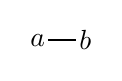
\begin{tikzpicture}[baseline=(a0.base), inner sep=1pt]
      \node (a0) {$a$};
      \node[right=1em of a0] (a1) {$b$};
      \path (a0) edge (a1);
   \end{tikzpicture}
   &
   $y=\sum_i a_i b_i$
   &
   $
\begin{compress}
\left[\begin{array}{cccc}
\cdot & \cdot & \cdot & \cdot \\
\end{array}\right]
\left[\begin{array}{c}
\cdot \\
\cdot \\
\cdot \\
\cdot \\
\end{array}\right]
\end{compress}
   $
   &
   $=y$
   \\
   Outer product
   &
   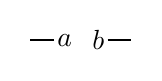
\begin{tikzpicture}[baseline=(a0.base), inner sep=1pt]
      \node (a0) {$a$};
      \node[right=.5em of a0] (a1) {$b$};
      \draw (a0.west) -- ++(-.3,0) node {};
      \draw (a1.east) -- ++(.3,0) node {};
   \end{tikzpicture}
   &
   $Y_{i,j} = a_i b_j$
   &
   $
\begin{compress}
\left[\begin{array}{c}
\cdot \\
\cdot \\
\cdot \\
\cdot \\
\end{array}\right]
\left[\begin{array}{cccc}
\cdot & \cdot & \cdot & \cdot \\
\end{array}\right]
\end{compress}
   $
   &
   $=\mathbin{
   \begin{tikzpicture}[baseline=(Y.base), inner sep=1pt]
      \node (Y) {$Y$};
      \draw (Y.east) -- ++(.3, 0);
      \draw (Y.west) -- ++(-.3, 0);
   \end{tikzpicture}}
   $
   \\
   Matrix-Vector
   &
   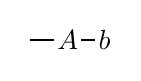
\begin{tikzpicture}[baseline=(A.base), inner sep=1pt]
      \node (A) {$A$};
      \node[right=.5em of A] (b) {$b$};
      \draw (A.west) -- ++(-.3,0) node {};
      \draw (A.east) -- (b.west);
   \end{tikzpicture}
   &
   $
   y_{i} = \sum_j A_{i,j} b_j
   $
   &
   $
   \begin{compress}
   \left[\begin{array}{cccc}
   \cdot & \cdot & \cdot & \cdot \\
   \cdot & \cdot & \cdot & \cdot \\
   \cdot & \cdot & \cdot & \cdot \\
   \cdot & \cdot & \cdot & \cdot \\
   \end{array}\right]
   \left[\begin{array}{c}
   \cdot \\
   \cdot \\
   \cdot \\
   \cdot \\
   \end{array}\right]
   \end{compress}
   $
   &
   $=\mathbin{
   \begin{tikzpicture}[baseline=(y.base), inner sep=1pt]
      \node (y) {$y$};
      \draw (y.west) -- ++(-.3, 0);
   \end{tikzpicture}
   }$
   \\
   Matrix-Matrix
   &
   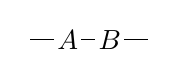
\begin{tikzpicture}[baseline=(A.base), inner sep=1pt]
      \node (A) {$A$};
      \node[right=.5em of A] (B) {$B$};
      \draw (A.west) -- ++(-.3,0) node {};
      \draw (A.east) -- (B.west);
      \draw (B.east) -- ++(.3,0) node {};
   \end{tikzpicture}
   &
   $
   Y_{i,k} = \sum_j A_{i,j} B_{j,k}
   $
   &
   $
   \begin{compress}
   \left[\begin{array}{cccc}
   \cdot & \cdot & \cdot & \cdot \\
   \cdot & \cdot & \cdot & \cdot \\
   \cdot & \cdot & \cdot & \cdot \\
   \cdot & \cdot & \cdot & \cdot \\
   \end{array}\right]
   \left[\begin{array}{cccc}
   \cdot & \cdot & \cdot & \cdot \\
   \cdot & \cdot & \cdot & \cdot \\
   \cdot & \cdot & \cdot & \cdot \\
   \cdot & \cdot & \cdot & \cdot \\
   \end{array}\right]
   \end{compress}
   $
   &
   $=\mathbin{
   \begin{tikzpicture}[baseline=(Y.base), inner sep=1pt]
      \node (Y) {$Y$};
      \draw (Y.west) -- ++(-.3, 0);
      \draw (Y.east) -- ++(.3, 0);
   \end{tikzpicture}
   }$
\end{tabular}
\vspace{.5em}

We think of vectors and matrices as tensors of order 1 and 2.
The order corresponds to the number of dimensions in their $[\cdots]$ visualization above,
e.g. a vector is a 1-dimensional list of numbers, while a matrix is a 2-dimensional grid of numbers.
The order also determines the degree of the node representing the variable in the tensor graph.

Diagram notation becomes more interesting when you have tensors of order 3 and higher.
An order 3 tensor is a cube or numbers, or stack of matrices.
E.g. we can write this as $T\in\R^{n\times m\times k}$, so $T_i\in\R^{m\times k}$ is a matrix for $i=1\dots n$.
Of course we could slice $T$ along the other axes too, so $T_{:,j}\in\R^{n\times k}$ and $T_{:,:,\ell}\in\R^{n\times m}$ are matrices too.

A matrix having two outgoing edges means there are two ways you can multiply a vector onto it, either on the left: $x^T M$, or on the right: $Mx$.
In graph notation we just write $x\!-\!M\!-$ and $-M\!-\!x$.
An order 3 tensor has three edges, so we can multiply it with a vector in three ways:
\[
   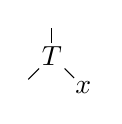
\begin{tikzpicture}[baseline=(T.base), inner sep=1pt]
      \node (T) {$T$};
      \node (x) at (.4,-.4) {$x$};
      \draw (T) -- (x);
      \draw (T) -- ++(-.3,-.3);
      \draw (T) -- ++(0,.35);
   \end{tikzpicture}
   \quad
   \text{and}
   \quad
   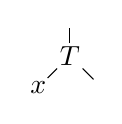
\begin{tikzpicture}[baseline=(T.base), inner sep=1pt]
      \node (T) {$T$};
      \node (x) at (-.4,-.4) {$x$};
      \draw (T) -- (x);
      \draw (T) -- ++(.3,-.3);
      \draw (T) -- ++(0,.35);
   \end{tikzpicture}
   \quad
   \text{and}
   \quad
   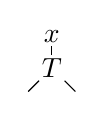
\begin{tikzpicture}[baseline=(T.base), inner sep=1pt]
      \node (T) {$T$};
      \node (x) at (0,.4) {$x$};
      \draw (T) -- (x);
      \draw (T) -- ++(.3,-.3);
      \draw (T) -- ++(-.3,-.3);
   \end{tikzpicture}
\]
%
To be perfectly precise about what each one means, we should give the edges labels.
For example we would write
$
   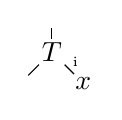
\begin{tikzpicture}[baseline=(T.base), inner sep=1pt]
      \node (T) {$T$};
      \node (x) at (.4,-.4) {$x$};
      \draw (T) -- (x) node[midway, above right, font=\tiny] {i};
      \draw (T) -- ++(-.3,-.3);
      \draw (T) -- ++(0,.3);
   \end{tikzpicture}
$
to specify the matrix $\sum_i T_i x_i$.
However, often the edge in question will be clear from the context, which is part of
what makes tensor diagram notation cleaner than, say, Einstein sum notation.

\[
   Y_{i,j} = \sum_{k,l,m,n,o} A_{i,k} B_{l,n,o} C_{j,k,l,m} D_{m,n} E_o
   \quad
   \Leftrightarrow
   % \quad
   \vcenter{\hbox{
      \import{figures/}{basic_graph.pdf_tex}
   }}
\]

The \emph{key principle} of tensor diagrams is that \emph{edge contraction is associative}.
This means you can contract any edge in any order you prefer.
This can be seen from the sum representation above, which can be reordered to sum over $k,l,m,n$ in any order.

The computational price for different contraction orders can be widely different.
Unfortunately it's not computationally easy to find the optimal order.
See section~\ref{sec:opt_contr} for algorithms to find the best contraction order, and approximate contraction methods.

Note that tensor graphs are not always connected.
We already saw that the outer product of two vectors can be written
   $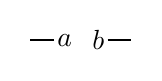
\begin{tikzpicture}[baseline=(a0.base), inner sep=1pt]
      \node (a0) {$a$};
      \node[right=.5em of a0] (a1) {$b$};
      \draw (a0.west) -- ++(-.3,0) node {};
      \draw (a1.east) -- ++(.3,0) node {};
   \end{tikzpicture}$.
This is natural from the sum representation: No edges simply means no sums.
So here $y_{i,j} = a_i b_j$, which is exactly the outer product $y=a\otimes b$.
% Can also mention how this gives us scaling by letter (5) be the order-0 tensor with value 5.


\section{The Copy Tensor}

A particularly important tensor is the ``copy'' tensor, also known as the ``diagonal'', ``kronecker delta'' or ``spider'' tensor.
The simplest version is the all-ones vector, which we write as $\sbullet-$.
That is $\sbullet_i = 1$.
The general order-n tensor is 1 on the diagonal, 0 everywhere else:
\[
   \sbullet_{i,j,k,\ldots} = \begin{cases}
      1\quad \text{if } i=j=k=\dots \\
      0\quad \text {otherwise}
   \end{cases}
\]
% This is also known as the ``copy'' or ``spider'' tensor, or ``generalized Kronecker delta''.
Or, using Iversonian notation,\footnote{%
For a logical proposition $P$, we define $
   [P] = \begin{cases}
      1 \text{ if } P \\
      0 \text{ otherwise}
   \end{cases}
$.} $\sbullet_{i,j,k,\dots} = [i=j=k=\dots]$.
We see the order-2 copy-tensor, $-\sbullet- = I$, is just the identity matrix,
so we can simply remove it from graphs like this:
\[-A\!-\!\sbullet\!-\!B- = -A\!-\!B-\]

Higher order copy-tensors are very useful, because they let us turn the simple tensor graphs into hyper-graphs.
A simple example of how we can use this is the diagonal matrix $D_a$, which has $a$ on the diagonal and 0 elsewhere.
We can write this as
\[
   D_a = 
   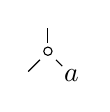
\begin{tikzpicture}[baseline=(T.base), inner sep=1pt]
      \node (T) {$\sbullet$};
      \node (x) at (.3,-.3) {$a$};
      \draw (T) -- (x);
      \draw (T) -- ++(-.25,-.25);
      \draw (T) -- ++(0,.3);
   \end{tikzpicture}
\]
Why?
Because $(D_a)_{i,j} = \sum_k \sbullet_{i,j,k} a_k = \sum_k [i=j=k] a_k = [i=j] a_i$.
Similarly the Hadamard product, $(a\circ b)_i = a_i b_i$, can be written
\[
   a \circ b =
   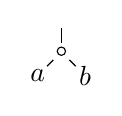
\begin{tikzpicture}[baseline=(T.base), inner sep=1pt]
      \node (T) {$\sbullet$};
      \node (a) at (-.3,-.3) {$a$};
      \node (b) at (.3,-.3) {$b$};
      \draw (T) -- (a);
      \draw (T) -- (b);
      \draw (T) -- ++(0,.3);
   \end{tikzpicture}
\]
Now, let's see why everyone loves copy tensors by using it to
prove the identity $D_aD_b = D_{a\circ b}$ by ``copy tensor manipulation'':
\[
   D_a D_b =
   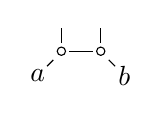
\begin{tikzpicture}[baseline=(T.base), inner sep=1pt]
      \node (T) {$\sbullet$};
      \node (a) at (-.3,-.3) {$a$};
      \draw (T) -- (a);
      \node (T2) at (.5,0) {$\sbullet$};
      \node (b) at (.8,-.3) {$b$};
      \draw (T) -- ++(0,.3);
      \draw (T) -- (T2);
      \draw (T2) -- (b);
      \draw (T2) -- ++(0,.3);
   \end{tikzpicture}
   =
   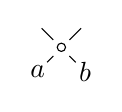
\begin{tikzpicture}[baseline=(T.base), inner sep=1pt]
      \node (T) {$\sbullet$};
      \node (a) at (-.3,-.3) {$a$};
      \node (b) at (.3,-.3) {$b$};
      \draw (T) -- (a);
      \draw (T) -- (b);
      \draw (T) -- ++(.25,.25);
      \draw (T) -- ++(-.25,.25);
   \end{tikzpicture}
   =
   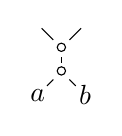
\begin{tikzpicture}[baseline=(T.base), inner sep=1pt]
      \node (T) {$\sbullet$};
      \node (a) at (-.3,-.3) {$a$};
      \node (b) at (.3,-.3) {$b$};
      \draw (T) -- (a);
      \draw (T) -- (b);
      \node (T2) at (0,.3) {$\sbullet$};
      \draw (T) -- (T2);
      \draw (T2) -- ++(.25,.25);
      \draw (T2) -- ++(-.25,.25);
   \end{tikzpicture}
   =
   D_{a\circ b}.
\]
You can verify this using the sum representation.

The general rule at play is that any connected sub-graph of copy-tensors can be combined into a single one.
Sometimes we are even lucky enough that this simplification leaves us with an identity matrix we can remove too:
%\begin{figure}[h]
%   \centering{
   %\def\svgwidth{.5\linewidth}
   %\import{figures/}{path1.pdf_tex}
   %\\
\[
   \def\svgwidth{.75\linewidth}
   \import{figures/}{path2.pdf_tex}
   .
\]
%   \caption{Contracting copy tensors and identity matrices}
%   \label{fig:spiders}
%   }
%\end{figure}
The only time you have to be a bit careful is when the resulting tensor has order 0.
Depending on how you define the order-0 copy tensor, $\sbullet$, you may or may not have the identity $\sbullet\!-\!\sbullet = \sbullet$.

Lots of other constructions that require special notation (like diagonal matrices or Hadamard products) with normal vector notation can be unified using the copy tensor.
%
In the Matrix Cookbook they define the order-4 tensor $J$,
which satisfies $J_{i,j,k,l} = [i=k][j=l]$ and which we'd write as
$J=\vcenter{\hbox{
   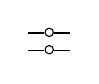
\begin{tikzpicture}[inner sep=0pt]
   \node (a0) {$\sbullet$};
   \draw (a0.east) -- ++(.2,0);
   \draw (a0.west) -- ++(-.2,0);
   \node[below=.2em of a0] (a1) {$\sbullet$};
   \draw (a1.east) -- ++(.2,0);
   \draw (a1.west) -- ++(-.2,0);
\end{tikzpicture}}}$,
and satisfies, for example, $\frac{dX}{dX}=J$.
Using ``tensor products'' you could write $J=I\otimes I$.
Note that $J$ is different from the order-4 copy-tensor,

\begin{tikzpicture}[baseline=(a0.base), inner sep=0pt]
   \node (a0) {$\sbullet$};
   \draw (a0) -- ++(.17,.17);
   \draw (a0) -- ++(.17,-.17);
   \draw (a0) -- ++(-.17,.17);
   \draw (a0) -- ++(-.17,-.17);
\end{tikzpicture}.

\section{Sums of Tensors}

Tensor products can express any linear function.
That is $f$ such that $f(a x, b y) = a b f(x,y)$.
Unfortunately not all operations on tensors are linear.
Even something as simple as a sum of two vectors, $x+y$, can not be displayed with a simple contraction graph.
(Note that this is not linear because $ax+by\neq ab(x+y)$.)

To handle this important operation, Penrose suggesting simply writing the two graphs with a plus sign between them, such as $-x + -y$.
Note that this is itself an order-1 tensor, even though it may look like there are two free edges.
If we want to multiply the sum with another tensor, we can use parentheses like $-M\!-\!(-x + -y)$.

It can be helpful to use named edges when dealing with sums, to make it clear how the edges are matched up.
Sums and tensor products interact nicely, with a general form of the distributive law:
%\begin{figure}[h]
%\centering{
%\def\svgwidth{\linewidth}
\[
\def\svgwidth{.75\linewidth}
\import{figures/}{path3.pdf_tex}
.
\]
%\caption{Distributive law}
%\label{fig:dist}
%}
%\end{figure}

When adding tensors that don't have the same number of edges, or have edges with different names, we can use ``broadcasting''.
%Say we want to add a matrix $\,_i\!-M-_j$ and a vector $x$.
Say we want to add a matrix $M$ and a vector $x$.
What does it even mean?
If we want to add $x$ to every row of $M$, we write
$
\vcenter{\hbox{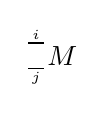
\begin{tikzpicture}[inner sep=1pt]
   \node (M) {$M$};
   \draw (M.north west) -- ++(-.2,0) node[midway, above, font=\tiny] {$i$};
   \draw (M.south west) -- ++(-.2,0) node[midway, below, font=\tiny] {$j$};
\end{tikzpicture}}}
+
\vcenter{\hbox{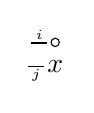
\begin{tikzpicture}[inner sep=1pt]
   \node (a0) {$\sbullet$};
   \draw (a0.west) -- ++(-.2,0) node[midway, above, font=\tiny] {$i$};
   \node[below=.2em of a0] (a1) {$x$};
   \draw (a1.west) -- ++(-.2,0) node[midway, below, font=\tiny] {$j$};
\end{tikzpicture}}}
$.
This is because
$
\vcenter{\hbox{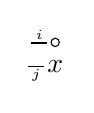
\begin{tikzpicture}[inner sep=1pt]
   \node (a0) {$\sbullet$};
   \draw (a0.west) -- ++(-.2,0) node[midway, above, font=\tiny] {$i$};
   \node[below=.2em of a0] (a1) {$x$};
   \draw (a1.west) -- ++(-.2,0) node[midway, below, font=\tiny] {$j$};
\end{tikzpicture}}}
$
is an outer product between $x$ and the all one vector, which is a matrix in which every row is the same.
Similarly, if we want to add $x$ to every column, we could use
the matrix
$
\vcenter{\hbox{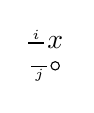
\begin{tikzpicture}[inner sep=1pt]
   \node (a0) {$\sbullet$};
   \draw (a0.west) -- ++(-.2,0) node[midway, below, font=\tiny] {$j$};
   \node[above=.2em of a0] (a1) {$x$};
   \draw (a1.west) -- ++(-.2,0) node[midway, above, font=\tiny] {$i$};
\end{tikzpicture}}}
$.

Note that we typically don't talk about ``rows'' or ``columns'' when dealing with tensors, but simply use the name edge (sometimes axis) of the tensor.
When using named edges, operations from classical vector notation like ``transpose'' can also be removed.
The matrix $X^T$ is simply $X$ where the left and right edge have been swapped.
But if the edges are named, we don't have to keep track on ``where the edge is'' at all.

\section{Transposition}
In classical matrix notation, transposition flips the indices of a matrix, so that
\[
   (A^T)_{ij} = A_{ji}.
\]
In tensor diagram notation, we have two choices depending on whether we want the position of the edges to be significant.
With significant edge positions, we typically let the ``left edge'' be the first index, and the ``right edge'' be the second index.
Thus transposition requires flipping the edges:
\[
   (\matmul{A})^T
   =
   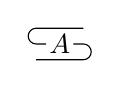
\begin{tikzpicture}[baseline=(a0.base), inner sep=1pt]
      \node (a0) {$A$};
      \draw (a0) -- ++(.3, 0) arc (270:90:-.1) --  ++(-.6, 0);
      \draw (a0) -- ++(-.3, 0) arc (270:90:.1) --  ++(.6, 0);
   \end{tikzpicture}
   =
   \matmul{A^T}.
\]
A fun notation used by some authors is flipping the tensor upside down, $\matmul{\vflip{A}}$, as a simpler way to flip the left and right edges.

In practical computations, keeping track of the edge positions can be easy to mess up.
It's more robust to name the ``outputs'' of the tensor, and let transposition rename the edges:
\[
   (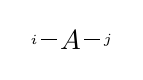
\begin{tikzpicture}[baseline=(A.base), inner sep=1pt]
   \node (A) {$A$};
   \draw (A.west) -- ++(-.2,0) node[left, font=\tiny] {$i$};
   \draw (A.east) -- ++(.2,0) node[right, font=\tiny] {$j$};
\end{tikzpicture})^T
=
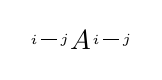
\begin{tikzpicture}[baseline=(A.base), inner sep=1pt]
   \node (A) {$A$};
   \node[font=\tiny] (i) at (-.2,0) {$j$};
   \node[font=\tiny] (j) at (.2,0) {$i$};
   \draw (i.west) -- ++(-.2,0) node[left, font=\tiny] {$i$};
   \draw (j.east) -- ++(.2,0) node[right, font=\tiny] {$j$};
\end{tikzpicture}
\]
%
Renaming can be done using multiplication by identity matrices:
\[
(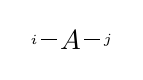
\begin{tikzpicture}[baseline=(A.base), inner sep=1pt]
   \node (A) {$A$};
   \draw (A.west) -- ++(-.2,0) node[left, font=\tiny] {$i$};
   \draw (A.east) -- ++(.2,0) node[right, font=\tiny] {$j$};
\end{tikzpicture})
(
\begin{tikzpicture}[baseline=(A.base), inner sep=1pt]
   \node (A) {$\sbullet$};
   \draw (A.west) -- ++(-.2,0) node[left, font=\tiny] {$j$};
   \draw (A.east) -- ++(.2,0) node[right, font=\tiny] {$k$};
\end{tikzpicture})
=
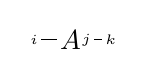
\begin{tikzpicture}[baseline=(A.base), inner sep=1pt]
   \node (A) {$A$};
   \draw (A.west) -- ++(-.2,0) node[left, font=\tiny] {$i$};
   \node[font=\tiny] (j) at (.2,0) {$j$};
   \draw (j) -- ++(.2,0) node[right, font=\tiny] {$k$};
\end{tikzpicture},
\]
but we have to be careful because overlapping edge names can make multiplication non-associative.
E.g.
\[
   \big[
(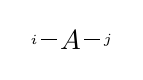
\begin{tikzpicture}[baseline=(A.base), inner sep=1pt]
   \node (A) {$A$};
   \draw (A.west) -- ++(-.2,0) node[left, font=\tiny] {$i$};
   \draw (A.east) -- ++(.2,0) node[right, font=\tiny] {$j$};
\end{tikzpicture})
(
\begin{tikzpicture}[baseline=(A.base), inner sep=1pt]
   \node (A) {$\sbullet$};
   \draw (A.west) -- ++(-.2,0) node[left, font=\tiny] {$j$};
   \draw (A.east) -- ++(.2,0) node[right, font=\tiny] {$k$};
\end{tikzpicture})
\big]
(
\begin{tikzpicture}[baseline=(A.base), inner sep=1pt]
   \node (A) {$\sbullet$};
   \draw (A.west) -- ++(-.2,0) node[left, font=\tiny] {$k$};
   \draw (A.east) -- ++(.2,0) node[right, font=\tiny] {$j$};
\end{tikzpicture})
=
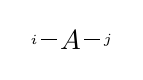
\begin{tikzpicture}[baseline=(A.base), inner sep=1pt]
   \node (A) {$A$};
   \draw (A.west) -- ++(-.2,0) node[left, font=\tiny] {$i$};
   \draw (A.east) -- ++(.2,0) node[right, font=\tiny] {$j$};
\end{tikzpicture}
\neq
(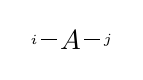
\begin{tikzpicture}[baseline=(A.base), inner sep=1pt]
   \node (A) {$A$};
   \draw (A.west) -- ++(-.2,0) node[left, font=\tiny] {$i$};
   \draw (A.east) -- ++(.2,0) node[right, font=\tiny] {$j$};
\end{tikzpicture})
   \big[
(
\begin{tikzpicture}[baseline=(A.base), inner sep=1pt]
   \node (A) {$\sbullet$};
   \draw (A.west) -- ++(-.2,0) node[left, font=\tiny] {$j$};
   \draw (A.east) -- ++(.2,0) node[right, font=\tiny] {$k$};
\end{tikzpicture})
(
\begin{tikzpicture}[baseline=(A.base), inner sep=1pt]
   \node (A) {$\sbullet$};
   \draw (A.west) -- ++(-.2,0) node[left, font=\tiny] {$k$};
   \draw (A.east) -- ++(.2,0) node[right, font=\tiny] {$j$};
\end{tikzpicture})
\big]
=
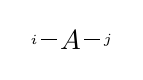
\begin{tikzpicture}[baseline=(A.base), inner sep=1pt]
   \node (A) {$A$};
   \draw (A.west) -- ++(-.2,0) node[left, font=\tiny] {$i$};
   \draw (A.east) -- ++(.2,0) node[right, font=\tiny] {$j$};
\end{tikzpicture}
\,

\begin{tikzpicture}[baseline=-0.6em, inner sep=1pt]
   \node (a0) {$\sbullet$};
   \node[below=.1 of a0] (a1) {$\sbullet$};
   \draw (a0) -- ++(.1, 0) arc (270:90:-.15) -- (a1);
   \draw (a1) -- ++(-.1, 0) arc (270:90:.15) -- (a0);
\end{tikzpicture},
\]
where
$
\begin{tikzpicture}[baseline=-0.7em, inner sep=1pt]
   \node (a0) {$\sbullet$};
   \node[below=.1 of a0] (a1) {$\sbullet$};
   \draw (a0) -- ++(.1, 0) arc (270:90:-.15) -- (a1);
   \draw (a1) -- ++(-.1, 0) arc (270:90:.15) -- (a0);
\end{tikzpicture}$
equals the matrix dimension.
In tensorgrad we solve this problem by requiring that any edge name is present at most twice in any product.

For the purpose of transcribing the matrix cookbook, using the ``significant position'' notation is more convenient.
We observe the following identities:
\begin{walign}
(A^T)^T &= A 
&
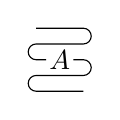
\begin{tikzpicture}[baseline=(a0.base), inner sep=1pt]
   \node (a0) {$A$};
   \draw (a0) -- ++(.3, 0) arc (270:90:-.1) -- ++(-.6, 0) arc (90:270:.1) -- ++(.6, 0);
   \draw (a0) -- ++(-.3, 0) arc (270:90:.1) -- ++(.6, 0) arc (90:270:-.1) -- ++(-.6, 0);
\end{tikzpicture}
&=
\matmul{A}
\\
%%%%%%%%%%%%%%%%%%%%%%%%%%%%%%%%%%%%%%%%%%%%%%%%%%%%%%%%%%%%%%%%%%%%%%%%%%%%%%%%
\tag{4}
(A + B)^T &= A^T + B^T
&
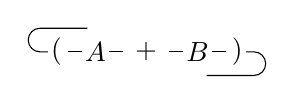
\begin{tikzpicture}[baseline=(a0.base), inner sep=1pt]
   \node (a0) {$\left( \matmul{A} + \matmul{B} \right)$};
   \draw (a0.east) -- ++(.1, 0) arc (270:90:-.15) -- ++(-.6, 0);
   \draw (a0.west) -- ++(-.1, 0) arc (270:90:.15) -- ++(.6, 0);
\end{tikzpicture}
&=
   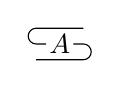
\begin{tikzpicture}[baseline=(a0.base), inner sep=1pt]
      \node (a0) {$A$};
      \draw (a0) -- ++(.3, 0) arc (270:90:-.1) --  ++(-.6, 0);
      \draw (a0) -- ++(-.3, 0) arc (270:90:.1) --  ++(.6, 0);
   \end{tikzpicture}
+
   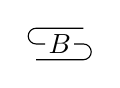
\begin{tikzpicture}[baseline=(a0.base), inner sep=1pt]
      \node (a0) {$B$};
      \draw (a0) -- ++(.3, 0) arc (270:90:-.1) --  ++(-.6, 0);
      \draw (a0) -- ++(-.3, 0) arc (270:90:.1) --  ++(.6, 0);
   \end{tikzpicture}
%\\
\end{walign}
\begin{walign}
%%%%%%%%%%%%%%%%%%%%%%%%%%%%%%%%%%%%%%%%%%%%%%%%%%%%%%%%%%%%%%%%%%%%%%%%%%%%%%%%
\tag{5}
(AB)^T &= B^T A^T
&
   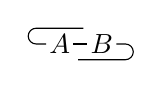
\begin{tikzpicture}[baseline=(a.base), inner sep=1pt]
      \node (a) {$A$};
      \node[right=.5em of a] (b) {$B$};
      \draw (a) -- (b);
      \draw (b) -- ++(.3, 0) arc (270:90:-.1) --  ++(-.6, 0);
      \draw (a) -- ++(-.3, 0) arc (270:90:.1) --  ++(.6, 0);
   \end{tikzpicture}
&=
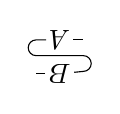
\begin{tikzpicture}[baseline=-.8em, inner sep=1pt]
   \node (a) {\vflip{$A$}};
   \node[below=.3em of a] (b) {\vflip{$B$}};
   \draw (a) -- ++(.3, 0);
   \draw (a) -- ++(-.3, 0) arc (90:270:.1) -- ++(.6, 0) arc (270:90:-.1) -- (b);
   \draw (b) -- ++(-.3, 0);
\end{tikzpicture}
=
\matmul{ \vflip{B}, \vflip{A} }
\end{walign}

\subsection{Higher order}
It is possible to generalize the idea of a transpose to higher order tensors.
It requires partitioning the edges as ``input'' and ``output'' edges, or more commonly, ``contravariant'' and ``covariant'' edges.
See the section at the end of this chapter for more on this.

We say matrices are symmetric if $A^T = A$.
For higher order tensors, there are many ways to be symmetric.
See the section~\ref{sec:symmetry} for more on this.

\section{Trace}

The ``trace'' of a square matrix is defined $\mathrm{Tr}(A) = \sum_i A_{i,i}$.
In tensor diagram notation, that corresponds to a self-edge: $\trace{A}{1}$.
The Matrix Cookbook has a list of identities using traces.
Let's reproduce them with tensor diagrams:
\begin{walign}
   \tag{11}
   \sum_{i=1}^{n} A_{ii} &= \mathrm{Tr}(A) = \mathrm{Tr}(A I)
   &
   \trace{A}{1} &= \trace{A, \sbullet}{2}
   \\
   %%%%%%%%%%%%%%%%%%%%%%%%%%%%%%%%%%%%%%%%
   \tag{13}
   \mathrm{Tr}(A) &= \mathrm{Tr}(A^T)
   &
   \trace{A}1
   \hspace{-1em}
   &=
   \hspace{-1em}
   \vflip{\trace{A}1}
   \\[0.5em]
   %%%%%%%%%%%%%%%%%%%%%%%%%%%%%%%%%%%%%%%%
   \tag{14}
   \mathrm{Tr}(AB)
   &=
   \mathrm{Tr}(BA)
   &
   \trace{A,B}2
   \hspace{-.5em}
   &=
   \hspace{.5em}
   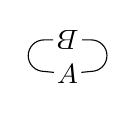
\begin{tikzpicture}[baseline=-1em, inner sep=1pt]
      \node (a) {$\vflip{B}$};
      \node[below=.3em of a] (b) {$A$};
      \draw (a) -- ++(-.3, 0) arc (90:270:.2) -- (b);
      \draw (a) -- ++(.3, 0) arc (270:90:-.2) -- (b);
   \end{tikzpicture}
   \hspace{.5em}
   =
   \hspace{-.5em}
   \trace{B,A}2
   \\[0.5em]
   %%%%%%%%%%%%%%%%%%%%%%%%%%%%%%%%%%%%%%%%
   \tag{15}
   \mathrm{Tr}(A+B)
   &= \mathrm{Tr}(A) + \mathrm{Tr}(B)
   &
   %\trace{(A+B),\sbullet}1
   %\trace{(\matmul{A}+\matmul{B}),\sbullet}1
   %\trace{(\matmul{A}+\matmul{B})}1
   %\trace{(\matmul{A}+\matmul{B}),\sbullet}{2}
   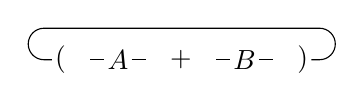
\begin{tikzpicture}[baseline=(a.base), inner sep=1pt]
      \node (a) {(\matmul{A}+\matmul{B})};
      \draw (a.west) -- ++(-.1, 0) arc (270:90:.2) -- ++(3.5, 0) arc (270:90:-.2) -- (a.east);
   \end{tikzpicture}
   &=
   \hspace{-1em}
   \trace{A}1
   \hspace{-1em}
   +
   \hspace{-1em}
   \trace{B}1
   \hspace{-1em}
   \\[0.5em]
   %%%%%%%%%%%%%%%%%%%%%%%%%%%%%%%%%%%%%%%%
   \tag{16}
   \mathrm{Tr}(ABC) &= \mathrm{Tr}(BCA)
   &
   \trace{A,B,C}1 &= \trace{B,C,A}1
   \\
                  & = \mathrm{Tr}(CAB)
                  &&= \trace{C,A,B}1
   \\[0.5em]
   %%%%%%%%%%%%%%%%%%%%%%%%%%%%%%%%%%%%%%%%
   \tag{17}
   a^T a &= \mathrm{Tr}(a a^T)
   &
   \vecmatvec{1em}{a}{}{a}
   &=
   \mathrm{Tr}(
   \begin{tikzpicture}[baseline=(a0.base), inner sep=1pt]
      \node (a0) {$a$};
      \node[right=.5em of a0] (a1) {$a$};
      \draw (a0.west) -- ++(-.3,0) node {};
      \draw (a1.east) -- ++(.3,0) node {};
   \end{tikzpicture}
   )
 \\&&&=
   \hspace{-1em}
   \begin{tikzpicture}[baseline=(a0.base), inner sep=1pt]
      \node (a0) {$a$};
      \node[right=1em of a0] (a1) {$a$};
      \path (a0) edge [out=160, in=20, looseness=2] (a1);
   \end{tikzpicture}
   \hspace{-1em}
\end{walign}

\subsection{Higher order traces}
For higher order tensors, we still define the trace as the sum of the diagonal elements.
That is, for a tensor $A$ of order $n$, the trace is just the product with the order $n$ copy tensor:
\[
   \begin{tikzpicture}[baseline=(T.base), inner sep=1pt]
      \node (Tr) {Tr(};
      \node[right=.3em of Tr] (T) {$T$};
      \node[right=.3em of T] (p) {)};
      \draw (T) -- ++(.3,-.3);
      \draw (T) -- ++(-.3,-.3);
      \draw (T) -- ++(0,.35);
   \end{tikzpicture}
   =
   \begin{tikzpicture}[baseline=(T.base), inner sep=1pt]
      \node (T) {$T$};
      \node[right=2em of T] (s) {$\sbullet$};
      \path (T) edge [out=90, in=120] (s);
      \path (T) edge [out=-30, in=200] (s);
      \path (T) edge [out=-120, in=220] (s);
   \end{tikzpicture}
   .
\]
In quantum mechanics, it is common to use a ``partial trace'', which we can define using index notation:
\[
   \begin{tikzpicture}[baseline=(T.base), inner sep=1pt]
      \node (Tr) {Tr$_{i,j}$(};
      \node[right=.3em of Tr] (T) {$T$};
      \node[right=.3em of T] (p) {)};
      \draw (T) -- ++(.3,-.3) node[midway, below left, font=\tiny] {j};
      \draw (T) -- ++(-.3,-.3) node[midway, below right, font=\tiny] {i};
      \draw (T) -- ++(0,.35) node[midway, above right, font=\tiny] {k};
   \end{tikzpicture}
   =
   \hspace{-.5em}
   \begin{tikzpicture}[baseline=(T.base), inner sep=1pt]
      \node (T) {$T$};
      \draw (T) -- ++(0,.35) node[midway, above right, font=\tiny] {k};
      \path (T) edge [out=-120, in=-60, loop] (T);
   \end{tikzpicture}
   .
\]
Of course with tensor diagrams, we can also use partial traces without naming the indices.
We don't even have to think about whether the contractions we use are traces or not.

\section{Eigenvalues}
Eigenvalues and eigenvectors are fundamental concepts in linear algebra that have important applications in tensor network theory. In tensor diagram notation, we can represent these concepts in a visually intuitive way.

For a matrix $A$, if there exists a non-zero vector $v$ and a scalar $\lambda$ such that $Av = \lambda v$, then $\lambda$ is called an eigenvalue of $A$, and $v$ is the corresponding eigenvector.
In tensor diagram notation It's convenient to write its eigendecomposition as $A = Q\Lambda Q^{-1}$, where $Q$ is a matrix whose columns are the eigenvectors of $A$, and $\Lambda$ is a diagonal matrix of the eigenvalues.
Thus:
\begin{align}
   \label{eq:eigen-decomposition}
   \begin{tikzpicture}[baseline=(A.base), inner sep=1pt]
   \node (A) {$A$};
   \draw (A.west) -- ++(-.3, 0);
   \draw (A.east) -- ++(+.3, 0);
   \end{tikzpicture}
   =
   \begin{tikzpicture}[baseline=(Q.base), inner sep=1pt]
   \node (Q) {$Q$};
   \draw (Q.west) -- ++(-.3, 0);
   \node[right=1em of Q] (dot) {$\sbullet$};
   \path (Q) edge (dot);
   \node[below=.3em of dot] (e) {$\lambda$};
   \path (dot) edge (e);
   \node[right=1em of dot] (Qi) {$Q^{-1}$};
   \path (dot) edge (Qi);
   \draw (Qi.east) -- ++(.3, 0);
   \end{tikzpicture}
\end{align}
The trace of a matrix is equal to the sum of its eigenvalues. We can represent this relationship using tensor diagrams:
\[
   \tag{12}
   \text{Tr}(A)
   =
   \hspace{-1em}
   \trace{A}{1}
   \hspace{-1em}
   =
   \hspace{-3em}
   \begin{tikzpicture}[baseline=(Q.base), inner sep=1pt]
      \node (Q) {$Q$};
      \node[right=1em of Q] (dot) {$\sbullet$};
      \path (Q) edge (dot);
      \node[below=.3em of dot] (e) {$\lambda$};
      \path (dot) edge (e);
      \node[right=1em of dot] (Qi) {$Q^{-1}$};
      \path (dot) edge (Qi);
      \path (Q.west) edge [out=160, in=20, looseness=2] (Qi.east);
   \end{tikzpicture}
   \hspace{-3em}
   =
   \hspace{-1em}
   \begin{tikzpicture}[baseline=(dot.base), inner sep=1pt]
      \node (dot) {$\sbullet$};
      \node[below=.3em of dot] (e) {$\lambda$};
      \path (dot) edge (e);
      \path (dot) edge [out=160, in=20, loop] ();
   \end{tikzpicture}
   \hspace{-1em}
   =
   \begin{tikzpicture}[baseline=(dot.base), inner sep=1pt]
      \node (dot) {$\sbullet$};
      \node[below=.3em of dot] (e) {$\lambda$};
      \path (dot) edge (e);
   \end{tikzpicture}
   =
   \sum_i \lambda_i
\]



\section{Symmetry and Symmetrization}
\label{sec:symmetry}

A common property of tensors is symmetry.
For matrices, symmetry means that $A^T = A$.
For tensors it means that permuting its indices does not change its value.
Typical examples are Covariance or Hessian matrices,
but also certain higher-order statistical moments, like the third or fourth moment tensors, can exhibit symmetries.
Sometimes only with respect to particular group, but most of the time with respect to all permutations of edges.
The Copy Tensor is a simple example of a completely symmetric tensor.

Sometimes it will be useful to symmetrize a tensor by summing over all permutations of its indices.
We write this using a squiggly line over the symmetrized edges:
\[
   \begin{tikzpicture}[baseline=.1em, inner sep=2pt, x=1em, y=.7em]
      \draw (0,0) -- ++(1,0);
      \draw (0,1) -- ++(1,0);
      \draw [very thick, line width=2pt, decorate, decoration={snake, amplitude=0.5mm, segment length=2.5mm}] (0.5,-.7) to (0.5,1.7);
   \end{tikzpicture}
   =
   \begin{tikzpicture}[baseline=.1em, inner sep=2pt, x=1em, y=.7em]
      \draw (0,0) -- ++(1,0);
      \draw (0,1) -- ++(1,0);
   \end{tikzpicture}
   +
   \begin{tikzpicture}[baseline=.1em, inner sep=2pt, x=1em, y=.7em]
      \draw (0,0) -- ++(1,1);
      \draw (0,1) -- ++(1,-1);
   \end{tikzpicture}
   ,\quad
   \begin{tikzpicture}[baseline=.5em, inner sep=2pt, x=1em, y=.7em]
      \draw (0,0) -- ++(1,0);
      \draw (0,1) -- ++(1,0);
      \draw (0,2) -- ++(1,0);
      \draw [very thick, line width=2pt, decorate, decoration={snake, amplitude=0.5mm, segment length=2.5mm}] (0.5,-.7) to (0.5,2.7);
   \end{tikzpicture}
   =
   \begin{tikzpicture}[baseline=.5em, inner sep=2pt, x=1em, y=.7em]
      \draw (0,0) -- ++(1,0);
      \draw (0,1) -- ++(1,0);
      \draw (0,2) -- ++(1,0);
   \end{tikzpicture}
   +
   \begin{tikzpicture}[baseline=.5em, inner sep=2pt, x=1em, y=.7em]
      \draw (0,0) -- ++(1,0);
      \draw (0,1) -- ++(1,1);
      \draw (0,2) -- ++(1,-1);
   \end{tikzpicture}
   +
   \begin{tikzpicture}[baseline=.5em, inner sep=2pt, x=1em, y=.7em]
      \draw (0,0) -- ++(1,1);
      \draw (0,1) -- ++(1,-1);
      \draw (0,2) -- ++(1,0);
   \end{tikzpicture}
   +
   \begin{tikzpicture}[baseline=.5em, inner sep=2pt, x=1em, y=.7em]
      \draw (0,0) -- ++(1,1);
      \draw (0,1) -- ++(1,1);
      \draw (0,2) -- ++(1,-2);
   \end{tikzpicture}
   +
   \begin{tikzpicture}[baseline=.5em, inner sep=2pt, x=1em, y=.7em]
      \draw (0,0) -- ++(1,2);
      \draw (0,1) -- ++(1,-1);
      \draw (0,2) -- ++(1,-1);
   \end{tikzpicture}
   +
   \begin{tikzpicture}[baseline=.5em, inner sep=2pt, x=1em, y=.7em]
      \draw (0,0) -- ++(1,2);
      \draw (0,1) -- ++(1,0);
      \draw (0,2) -- ++(1,-2);
   \end{tikzpicture}
\]
For example, if $A$ is a square matrix,
\(
   A + A^T =
   \begin{tikzpicture}[baseline=(A.base), inner sep=2pt, x=2em, y=2em]
      \node (A) at (0,0) {$A$};
      \draw (A) -- ++(-1,0);
      \draw (A) -- ++(1,0);
    \draw [very thick, decorate, decoration={snake, amplitude=.5mm, segment length=2.1mm}]
        ($(A)+(.6,-.3)$) arc [start angle=-20, end angle=200, x radius=0.6, y radius=0.5];
   \end{tikzpicture}
   =
   \begin{tikzpicture}[baseline=(A.base), inner sep=2pt, x=1.5em, y=2em]
      \node (A) at (0,0) {$A$};
      \draw (A) -- ++(-1,0);
      \draw (A) -- ++(1,0);
   \end{tikzpicture}
   +
   \begin{tikzpicture}[baseline=(a0.base), inner sep=1pt]
      \node (a0) {$A$};
      \draw (a0) -- ++(.3, 0) arc (270:90:-.1) --  ++(-.6, 0);
      \draw (a0) -- ++(-.3, 0) arc (270:90:.1) --  ++(.6, 0);
   \end{tikzpicture}
   .
\)
There is a complementary notion of \emph{anti-symmetrization} (or \emph{skew-symmetrization}), where we sum over \emph{all permutations with appropriate sign}.
For instance, a rank-2 skew-symmetric matrix \(A\) satisfies \(A_{ij} = -A_{ji}\).
We can anti-symmetrize using a flat thick line:
\(
   \begin{tikzpicture}[baseline=(A.base), inner sep=2pt, x=2em, y=2em]
      \node (A) at (0,0) {$A$};
      \draw (A) -- ++(-1,0);
      \draw (A) -- ++(1,0);
    \draw [very thick] ($(A)+(.6,-.2)$) arc [start angle=-10, end angle=190, x radius=0.6, y radius=0.5];
   \end{tikzpicture}
   =
   \begin{tikzpicture}[baseline=(A.base), inner sep=2pt, x=1.5em, y=2em]
      \node (A) at (0,0) {$A$};
      \draw (A) -- ++(-1,0);
      \draw (A) -- ++(1,0);
   \end{tikzpicture}
   -
   \begin{tikzpicture}[baseline=(a0.base), inner sep=1pt]
      \node (a0) {$A$};
      \draw (a0) -- ++(.3, 0) arc (270:90:-.1) --  ++(-.6, 0);
      \draw (a0) -- ++(-.3, 0) arc (270:90:.1) --  ++(.6, 0);
   \end{tikzpicture}
   .
\)
In higher-rank cases, the sign of each term is determined by the parity of the permutation.

Both tensors are idempotent, since symmetrizing a symmetric tensor has no effect:
\[
   \begin{tikzpicture}[baseline=.5em, inner sep=2pt, x=1em, y=.7em]
      \draw (0,0) -- ++(2,0);
      \draw (0,1) -- ++(2,0);
      \draw (0,2) -- ++(2,0);
      \draw [very thick, line width=2pt, decorate, decoration={snake, amplitude=0.5mm, segment length=2.5mm}] (0.66,-.7) to (0.66,2.7);
      \draw [very thick, line width=2pt, decorate, decoration={snake, amplitude=0.5mm, segment length=2.5mm}] (1.33,-.7) to (1.33,2.7);
   \end{tikzpicture}
   =
   \begin{tikzpicture}[baseline=.5em, inner sep=2pt, x=1em, y=.7em]
      \draw (0,0) -- ++(1,0);
      \draw (0,1) -- ++(1,0);
      \draw (0,2) -- ++(1,0);
      \draw [very thick, line width=2pt, decorate, decoration={snake, amplitude=0.5mm, segment length=2.5mm}] (0.5,-.7) to (0.5,2.7);
   \end{tikzpicture}
   ,\quad
   \begin{tikzpicture}[baseline=.5em, inner sep=2pt, x=1em, y=.7em]
      \draw (0,0) -- ++(2,0);
      \draw (0,1) -- ++(2,0);
      \draw (0,2) -- ++(2,0);
      \draw [very thick] (0.66,-.7) to (0.66,2.7);
      \draw [very thick] (1.33,-.7) to (1.33,2.7);
   \end{tikzpicture}
   =
   \begin{tikzpicture}[baseline=.5em, inner sep=2pt, x=1em, y=.7em]
      \draw (0,0) -- ++(1,0);
      \draw (0,1) -- ++(1,0);
      \draw (0,2) -- ++(1,0);
      \draw [very thick] (0.5,-.7) to (0.5,2.7);
   \end{tikzpicture}
   .
\]


\section{Covariance and Contravariance}

In physics it's often relevant to change between different coordinate systems.
Most such changes transform the left and right side of matrices differently, and similarly row and column vectors.
For tensors this generalize to the concepts of covariance and contravariance.
With notion, we keep track of ``input'' and ``output'' vectors.
We'll also need to distinguish between things such as the identity matrix, $\matmul{\sbullet}$,
$\begin{tikzpicture}[baseline=(a0.base), inner sep=0pt]
   \node (a0) {$\sbullet$};
   \draw (a0) -- ++(-.17,.1);
   \draw (a0) -- ++(-.17,-.1);
\end{tikzpicture}$,
and
$\begin{tikzpicture}[baseline=(a0.base), inner sep=0pt]
   \node (a0) {$\sbullet$};
   \draw (a0) -- ++(.17,.1);
   \draw (a0) -- ++(.17,-.1);
\end{tikzpicture}$.

This notion allows some ability to ``algebraically'' combine tensors, by connecting input edges to output edges, just like we do with matrices and vectors.
However, for more complicated tensors, we need to know which edges to combine, and index notation is more useful.

In computer science and machine learning, the concept of covariance and contravariance is typically not useful, so we won't use it in this book.

\section{Exercises}
\begin{exercise}
   Given a sequence of matrices $A_1, A_2, \ldots, A_n \in \mathbb R^{n\times n}$,
   and vectors $v_1, v_2, \ldots, v_n \in \mathbb R^n$,
   draw, using tensor diagrams, the matrix made of vectors $A_1v_1, A_2v_2, \ldots, A_nv_n$.
\end{exercise}
\begin{exercise}
Represent the Hadamard product (element-wise multiplication) of two matrices using tensor diagrams.
How does this differ from regular matrix multiplication?
(We will see more about this in \ref{sec:hadamard}.)
\end{exercise}
\begin{exercise}
Represent the SVD of a matrix $A = U\Sigma V^T$ using tensor diagrams.
How does this compare to the eigendecomposition diagram?
How can you generalize it to higher order tensors?
(In section \ref{sec:HOSVD} we will see more about this.)
\end{exercise}


\chapter{Simple Derivatives}

A derivative with respect to a tensor is simply the collection of derivatives with respect to each element of this tensor.
We can keep track of $\frac{d T}{d U}$ by making a tensor of shape $\mathrm{shape}(T) \cup \mathrm{shape}(U)$.
For example, if $T$ is an order-3 tensor and $U$ is an order-2 tensor, we draw $dT/dU$ as
\[
   \frac{dT}{dU} =
   \vcenter{\hbox{
      \import{figures/}{dTdU.pdf_tex}
   }}
\]
This notation follows Penrose.
The two extra lines coming from the black dot on the circle makes the derivative an order-5 tensor.
That the order of derivatives grows this way, is one of the main reasons we'll encounter for tensors to show up in the first place.

When there are not too many edges, we will use a simple inline notation like this:
\[
\begin{tikzpicture}[baseline=(T.base), inner sep=1pt]
   \node (T) {$(T)$};
   \draw (T) -- ++(-.5,-.1);
   \draw (T) -- ++(-.5,+.1);
   \draw (T) -- ++(+.5,0);
   \draw[d] (T.east) -- ++(.2,.2);
   \draw[d] (T.east) -- ++(.3,.1);
\end{tikzpicture}
\]

The Matrix Cookbook defines the single-entry matrix $J^{i,j} \in R^{n\times n}$ as the matrix which is zero everywhere except in the entry $(i, j)$ in which it is 1.
Alternatively we could write $J^{i,j}_{n,m} = [i=n][j=m]$.

\section{Derivatives of Matrices, Vectors and Scalar Forms}

\subsection{First Order}
The following first order derivatives show the basic linearity properties of the derivative operator.

\begin{walign}
   \tag{69}
   \frac{\partial x^T a}{\partial x}
   &= a
   &
      \begin{tikzpicture}[baseline=(a0.base), inner sep=1pt]
         \node (a0) {$(x$};
         \node[right=1em of a0] (a1) {$a)$};
         \path (a0) edge (a1);
         \draw [d] (a1.east) -- ++(-.2,.2);
      \end{tikzpicture}
   &=
      \begin{tikzpicture}[baseline=(a0.base), inner sep=1pt]
         \node (a0) {$(x)$};
         \node[right=1em of a0] (a1) {$a$};
         \path (a0) edge (a1);
         \draw [d] (a0.east) -- ++(-.2,.2);
      \end{tikzpicture}
   =
      \begin{tikzpicture}[baseline=(a.base), inner sep=1pt]
         \draw (0,0) node[right] (a) {$a$} -- ++(-.3, 0);
      \end{tikzpicture}
   \\
   %%%%%%%%%%%%%%%%%%%%%%%%%%%%%%%%%%%%%%%%
   \tag{69}
   \frac{\partial a^T x}{\partial x}
   &= a
   &
      \begin{tikzpicture}[baseline=(a0.base), inner sep=1pt]
         \node (a0) {$(a$};
         \node[right=1em of a0] (a1) {$x)$};
         \path (a0) edge (a1);
         \draw [d] (a1.east) -- ++(-.2,.2);
      \end{tikzpicture}
   &=
      \begin{tikzpicture}[baseline=(a0.base), inner sep=1pt]
         \node (a0) {$(x)$};
         \node[left=1em of a0] (a1) {$a$};
         \path (a0) edge (a1);
         \draw [d] (a0.east) -- ++(-.2,.2);
      \end{tikzpicture}
   =
      \begin{tikzpicture}[baseline=(a.base), inner sep=1pt]
         \node (a) {$a$};
         \draw (a.east) -- ++(.1, 0) arc (270:90:-.1) -- ++(-.1, 0);
      \end{tikzpicture}
   =
      \begin{tikzpicture}[baseline=(a.base), inner sep=1pt]
         \draw (0,0) node[right] (a) {$a$} -- ++(-.3, 0);
      \end{tikzpicture}
   \\
   %%%%%%%%%%%%%%%%%%%%%%%%%%%%%%%%%%%%%%%%
   \tag{70}
   \frac{\partial a^T X b}{\partial X} &= ab^T
   &
      \begin{tikzpicture}[baseline=(a0.base), inner sep=1pt]
         \node (a0) {$(a$};
         \node[right=1em of a0] (a1) {$X$};
         \node[right=1em of a1] (a2) {$b)$};
         \path (a0) edge (a1);
         \path (a1) edge (a2);
         \draw[d] (a2.east) -- ++(.2,.2);
         \draw[d] (a2.east) -- ++(.3,.1);
      \end{tikzpicture}
   &=
      \begin{tikzpicture}[baseline=(a0.base), inner sep=1pt]
         \node (a0) {$a$};
         \node[right=1em of a0] (a1) {$(X)$};
         \node[right=1em of a1] (a2) {$b$};
         \path (a0) edge (a1);
         \path (a1) edge (a2);
         \draw[d] (a1.east) -- ++(.2,.2);
         \draw[d] (a1.east) -- ++(.3,.1);
      \end{tikzpicture}
      =
      \begin{tikzpicture}[baseline=(a.base), inner sep=1pt]
         \node (a) {$a$};
         \draw (a) -- ++(.3, 0) arc (270:90:-.1);
         \node[right=2em of a] (b) {$b$};
         \draw (b) -- ++(-.3, 0) arc (270:90:.1);
      \end{tikzpicture}
   \\
   %%%%%%%%%%%%%%%%%%%%%%%%%%%%%%%%%%%%%%%%
   \tag{73}
   \frac{\partial X}{\partial X_{i,j}} &= J^{i,j}
   &
      \begin{tikzpicture}[baseline=(a0.base), inner sep=1pt]
         \node (a0) {$($};
         \node[right=1em of a0] (a1) {$X$};
         \node[right=1em of a1] (a2) {$)$};
         \draw (a0) -- (a1) -- (a2);
         \draw[d] (a2.east) -- ++(.2,.2) node[midway, above left, font=\tiny] {i};
         \draw[d] (a2.east) -- ++(.3,.1) node[midway, below right, font=\tiny] {j};
      \end{tikzpicture}
   &=
      \begin{tikzpicture}[baseline=(a.base), inner sep=1pt]
         \node (a) {};
         \draw (a) -- ++(.3, 0) arc (270:90:-.1) node[pos=1, below left, font=\tiny] {i};
         \node[right=2em of a] (b) {};
         \draw (b) -- ++(-.3, 0) arc (270:90:.1) node[pos=1, above right, font=\tiny] {j};
      \end{tikzpicture}
   \\
   %%%%%%%%%%%%%%%%%%%%%%%%%%%%%%%%%%%%%%%%
   \tag{74}
   \frac{\partial (X A)_{i,j}}{\partial X_{m,n}} &= (J^{m,n} A)_{i,j}
   &
      \begin{tikzpicture}[baseline=(a0.base), inner sep=1pt]
         \node (a0) {$($};
         \node[right=1em of a0] (a1) {$X$};
         \node[right=1em of a1] (a2) {$A$};
         \node[right=1em of a2] (a3) {$)$};
         \draw (a0) -- (a1) node[midway, above left, font=\tiny] {i};
         \draw (a1) -- (a2);
         \draw (a2) -- (a3) node[midway, below right, font=\tiny] {j};
         \draw[d] (a3.east) -- ++(.2,.2) node[midway, above left, font=\tiny] {m};
         \draw[d] (a3.east) -- ++(.3,.1) node[midway, below right, font=\tiny] {n};
      \end{tikzpicture}
   &=
      \begin{tikzpicture}[baseline=(a0.base), inner sep=1pt]
         \node (a0) {};
         \node[right=1em of a0] (a1) {$(X)$};
         \node[right=1em of a1] (a2) {$A$};
         \node[right=1em of a2] (a3) {};
         \path (a0) edge (a1);
         \path (a1) edge (a2);
         \path (a2) edge (a3);
         \draw[d] (a1.east) -- ++(.2,.2);
         \draw[d] (a1.east) -- ++(.3,.1);
      \end{tikzpicture}
 \\&&&=
      \begin{tikzpicture}[baseline=(a0.base), inner sep=1pt]
         \node (a0) {};
         \node[right=1.5em of a0] (a2) {$A$};
         \draw (a0) -- ++(-.1,0) node[midway, above left, font=\tiny] {i};
         \draw (a2) -- ++(.5,0) node[midway, below right, font=\tiny] {j};
         \draw (a0.west) -- ++(.2,0) arc (90:270:-.1) node[pos=1, above right, font=\tiny] {m};
         \draw (a2.west) -- ++(-.2,0) arc (90:270:.1) node[midway, below left, font=\tiny] {n};
      \end{tikzpicture}
\end{walign}

\subsection{Second Order}
The second order derivatives are follow from the product rule:
\[
   \vcenter{\hbox{
      \import{figures/}{product.pdf_tex}
   }}
\]
Note that this rule holds independently of how many edges are between $T$ and $U$, even if there are none.

\begin{walign}
   \tag{76}
   \frac{\partial}{\partial X_{i,j}}
   \sum_{k,l,m,n} X_{k,l} X_{m,n}
   &= (\sum_{k,l} X_{k,l})^2
   %&= \frac{\partial \|X\|_F^2}{\partial X_{i,j}}
   %&= 2\, \sum_{k,l} X_{k,l}
   &
   \begin{tikzpicture}[baseline=.5em, inner sep=1pt]
      \node (a0) at (0,0) {$\sbullet$};
      \node (a1) at (.5,0) {$X$};
      \node (a2) at (1,0) {$\sbullet$};
      \path (a0) edge (a1);
      \path (a1) edge (a2);
      \node (b0) at (0, .5) {$\sbullet$};
      \node (b1) at (.5, .5) {$X$};
      \node (b2) at (1, .5) {$\sbullet$};
      \path (b0) edge (b1);
      \path (b1) edge (b2);
      \node at (-.25, .25) {$\bigg($};
      \node at (1.25, .25) {$\bigg)$};
      \draw[d] (1.35, .4) -- ++(.2,.2) node[midway, above left, font=\tiny] {i};
      \draw[d] (1.35, .4) -- ++(.3,.1) node[midway, below right, font=\tiny] {j};
   \end{tikzpicture}
   &=
   \begin{tikzpicture}[baseline=.5em, inner sep=1pt]
      \node (a0) at (0,0) {$\sbullet$};
      \node (a1) at (.5,0) {$(X)$};
      \node (a2) at (1,0) {$\sbullet$};
      \path (a0) edge (a1);
      \path (a1) edge (a2);
      \node (b0) at (0, .5) {$\sbullet$};
      \node (b1) at (.5, .5) {$X$};
      \node (b2) at (1, .5) {$\sbullet$};
      \path (b0) edge (b1);
      \path (b1) edge (b2);
      \draw[d] (.83,.0) -- ++(.2,.2);
      \draw[d] (.83,.0) -- ++(.3,.1);
   \end{tikzpicture}
   +
   \begin{tikzpicture}[baseline=.5em, inner sep=1pt]
      \node (a0) at (0,0) {$\sbullet$};
      \node (a1) at (.5,0) {$X$};
      \node (a2) at (1,0) {$\sbullet$};
      \path (a0) edge (a1);
      \path (a1) edge (a2);
      \node (b0) at (0, .5) {$\sbullet$};
      \node (b1) at (.5, .5) {$(X)$};
      \node (b2) at (1, .5) {$\sbullet$};
      \path (b0) edge (b1);
      \path (b1) edge (b2);
      \draw[d] (0.83,.5) -- ++(.2,.2);
      \draw[d] (0.83,.5) -- ++(.3,.1);
   \end{tikzpicture}
   %\\[.3em]
   \\
   &= 2\, \sum_{k,l} X_{k,l}
   &&=
   2\,
   \begin{tikzpicture}[baseline=.5em, inner sep=1pt]
      \node (a0) at (0,0) {$\sbullet$};
      \node (a1) at (.5,0) {};
      \node (a2) at (1,0) {$\sbullet$};
      \path (a0) edge (a1);
      \path (a1) edge (a2);
      \node (b0) at (0, .5) {$\sbullet$};
      \node (b1) at (.5, .5) {$X$};
      \node (b2) at (1, .5) {$\sbullet$};
      \path (b0) edge (b1);
      \path (b1) edge (b2);
      \draw (a1.west) -- ++(.1,.2) node[midway, above left, font=\tiny] {i};
      \draw (a1.east) -- ++(-.1,-.2) node[midway, below right, font=\tiny] {j};
   \end{tikzpicture}
   %%%%%%%%%%%%%%%%%%%%%%%%%%%%%%%%%%%%%%%%
   \\[.5em]
   \tag{77} 
   \frac{\partial b^T X^T X c}{\partial X} &= X(bc^T + cb^T) 
   &
   \begin{tikzpicture}[baseline=(a0.base), inner sep=1pt]
      \node (a0) {$(\vecmatvec{.5em}{b}{X^T,X}{c})$};
      \draw[d] (a0.east) -- ++(.2,.2);
      \draw[d] (a0.east) -- ++(.3,.1);
   \end{tikzpicture}
   &=
   \begin{tikzpicture}[baseline=(a0.base), inner sep=1pt]
      \node (a0) {$b$};
      \node[right=1em of a0] (a1) {$X^T$};
      \node[right=1em of a1] (a2) {$(X)$};
      \node[right=1em of a2] (a3) {$c$};
      \draw (a0) -- (a1);
      \draw (a1) -- (a2);
      \draw (a2) -- (a3);
      \draw[d] (a2.east) -- ++(.2,.2);
      \draw[d] (a2.east) -- ++(.3,.1);
   \end{tikzpicture}
 \\&&&+
   \begin{tikzpicture}[baseline=(a0.base), inner sep=1pt]
      \node (a0) {$b$};
      \node[right=1em of a0] (a1) {$(X^T)$};
      \node[right=1em of a1] (a2) {$X$};
      \node[right=1em of a2] (a3) {$c$};
      \draw (a0) -- (a1);
      \draw (a1) -- (a2);
      \draw (a2) -- (a3);
      \draw[d] (a1.east) -- ++(.2,.2);
      \draw[d] (a1.east) -- ++(.3,.1);
   \end{tikzpicture}
   \\[.3em]&&&=
   \begin{tikzpicture}[baseline=(a0.base), inner sep=1pt]
      \node (a0) {$b$};
      \node[right=1em of a0] (a1) {$X^T$};
      \node[right=1em of a1] (a2) {};
      \node[right=1em of a2] (a3) {$c$};
      \draw (a0) -- (a1);
      \draw (a1) -- (a2);
      \draw (a2) -- (a3);
      \draw (a2.west) -- ++(.1,.2);
      \draw (a2.east) -- ++(-.1,-.2);
   \end{tikzpicture}
 \\&&&+
   \begin{tikzpicture}[baseline=(a0.base), inner sep=1pt]
      \node (a0) {$b$};
      \node[right=1em of a0] (a1) {};
      \node[right=1em of a1] (a2) {$X$};
      \node[right=1em of a2] (a3) {$c$};
      \draw (a0) -- (a1);
      \draw (a1) -- (a2);
      \draw (a2) -- (a3);
      \draw (a1.west) -- ++(.1,.2);
      \draw (a1.east) -- ++(-.1,-.2);
   \end{tikzpicture}
   \\[.3em]&&&=
   \begin{tikzpicture}[baseline=(a0.base), inner sep=1pt]
      \node (a0) {$X$};
      \node[right=.7em of a0] (a1) {$($};
      \node[right=.4em of a1] (a2) {$b\, c$};
      \node[right=.4em of a2] (a4) {$+$};
      \node[right=.6em of a4] (a5) {$c\, b$};
      \node[right=.2em of a5] (a7) {$)$};
      \draw (a0.west) -- ++(-.2,0);
      \draw (a0) -- (a1);
      \draw (a2.west) -- ++(-.2,0);
      \draw (a2.east) -- ++(.1,.15);
      \draw (a5.west) -- ++(-.2,0);
      \draw (a5.east) -- ++(.1,.15);
   \end{tikzpicture}
   \\
   \tag{79} 
   \frac{\partial}{\partial X_{i,j}} (X^TBX)_{k,l} &= \delta_{l,j}(X^TB)_{k,i}
   %  \\&+ \delta_{k,j}(BX)_{i,l} 
   &
   \begin{tikzpicture}[baseline=(a0.base), inner sep=1pt]
      \node (a0) {$($};
      \node[right=.5em of a0] (a1) {$X^T$};
      \node[right=.5em of a1] (a2) {$B$};
      \node[right=.5em of a2] (a3) {$X$};
      \node[right=.5em of a3] (a4) {$)$};
      \draw (a0) -- (a1) node[midway, above left, font=\tiny] {k};
      \draw (a1) -- (a2);
      \draw (a2) -- (a3);
      \draw (a3) -- (a4) node[midway, below right, font=\tiny] {l};
      \draw[d] (a4.east) -- ++(.2,.2) node[midway, above left, font=\tiny] {i};
      \draw[d] (a4.east) -- ++(.3,.1) node[midway, below right, font=\tiny] {j};
   \end{tikzpicture}
   &=
   \begin{tikzpicture}[baseline=(a0.base), inner sep=1pt]
      \node (a0) {};
      \node[right=.5em of a0] (a1) {$X^T$};
      \node[right=.5em of a1] (a2) {$B$};
      \node[right=.5em of a2] (a3) {};
      \node[right=.5em of a3] (a4) {};
      \draw (a0) -- (a1) node[midway, above left, font=\tiny] {k};
      \draw (a1) -- (a2);
      \draw (a2) -- (a3);
      \draw (a3) -- (a4) node[midway, below right, font=\tiny] {l};
      \draw (a3.west) -- ++(.1,.2) node[midway, above left, font=\tiny] {i};
      \draw (a3.east) -- ++(-.1,-.2) node[midway, below right, font=\tiny] {j};
   \end{tikzpicture}
   \\
   &+ \delta_{k,j}(BX)_{i,l}
   &&+
   \begin{tikzpicture}[baseline=(a0.base), inner sep=1pt]
      \node (a0) {};
      \node[right=.5em of a0] (a1) {};
      \node[right=.5em of a1] (a2) {$B$};
      \node[right=.5em of a2] (a3) {$X$};
      \node[right=.5em of a3] (a4) {};
      \draw (a0) -- (a1) node[midway, above left, font=\tiny] {k};
      \draw (a1) -- (a2);
      \draw (a2) -- (a3);
      \draw (a3) -- (a4) node[midway, below right, font=\tiny] {l};
      \draw (a1.west) -- ++(.1,.2) node[midway, above left, font=\tiny] {j};
      \draw (a1.east) -- ++(-.1,-.2) node[midway, below right, font=\tiny] {i};
   \end{tikzpicture}
   %%%%%%%%%%%%%%%%%%%%%%%%%%%%%%%%%%%%%%%%
   \\
   \tag{80}
   \frac{\partial}{\partial X_{i,j}} X^TBX &= X^TBJ^{i,j} + J^{j,i}BX 
   &
   \text{(same as above)} &
   %%%%%%%%%%%%%%%%%%%%%%%%%%%%%%%%%%%%%%%%
   \\
   \tag{81}
   \frac{\partial}{\partial x} x^TBx &= (B+B^T)x 
   &
   \begin{tikzpicture}[baseline=(a0.base), inner sep=1pt]
      \node (a0) {$(x$};
      \node[right=.5em of a0] (a1) {$B$};
      \node[right=.5em of a1] (a2) {$x)$};
      \draw (a0) -- (a1);
      \draw (a1) -- (a2);
      \draw[d] (a2.east) -- ++(.2,.2);
   \end{tikzpicture}
   &=
   \vecmatvec{.5em}{}{B}{x}
   +
   \begin{tikzpicture}[baseline=(a0.base), inner sep=1pt]
      \node (a0) {$x$};
      \node[right=.5em of a0] (a1) {$B$};
      \draw (a0) -- (a1) -- ++(.3,0) arc (270:90:-.1) -- ++(-.3,0);
   \end{tikzpicture}
 \\&&&=
 \vecmatvec{.5em}{
    (\vecmatvec{.5em}{}{B}{}
    + \vecmatvec{.5em}{}{B^T}{})}
    {}{x}
 \\&&&=
   \begin{tikzpicture}[baseline=.5em, inner sep=1pt]
      \node (a0) at (0,0) {};
      \node (a1) at (.5,0) {$B$};
      \node (a2) at (1,0) {};
      \draw (a0) -- (a1) node[midway, below left, font=\tiny] {i};
      \draw (a1) -- (a2) node[midway, below right, font=\tiny] {j};
      \node (b0) at (0, .5) {};
      \node (b1) at (.5, .5) {$B$};
      \node (b2) at (1, .5) {};
      \draw (b0) -- (b1) node[midway, above left, font=\tiny] {j};
      \draw (b1) -- (b2) node[midway, above right, font=\tiny] {i};
      \node (l) at (-.3, .25) {$\bigg($};
      \node at (1.15, .25) {$\bigg)$};
      \node at (-.1, .25) {$+$};
      \node (x) at (-1,.25) {$x$};
      \draw (x) -- (l) node[midway, above right, font=\tiny] {i};
   \end{tikzpicture}
\end{walign}


TODO: Assume $W$ is symmetric, then... (84) - (88)

\subsection{Higher Order}
Integer powers of matrices, like $X^n$, are easy to handle by writing
out the product and using the product rule.
The Matrix Cookbook includes a few derivatives we can handle this way.
\begin{walign}
   \\[.5em]
   \tag{90}
   \frac{\partial\left(\mathbf{X}^n\right)_{k l}}{\partial X_{i j}}
   &=
  \sum_{r=0}^{n-1}\left(\mathbf{X}^r \mathbf{J}^{i j} \mathbf{X}^{n-1-r}\right)_{k l}
   &&
   \begin{tikzpicture}[baseline=(X0.base), inner sep=1pt]
      \node (X0) {$(X$};
      \node[right=.25 of X0] (X1) {$X$};
      \node[right=.25 of X1] (X2) {$X$};
      \node[right=.25 of X2] (X3) {$\dots$};
      \node[right=.25 of X3] (X4) {$X)$};
      \draw (X0) -- ++(-.5,0) node[midway, above left, font=\tiny] {k};
      \draw (X0) -- (X1) -- (X2) -- (X3) -- (X4);
      \draw (X4) -- ++(.5,0) node[midway, below right, font=\tiny] {l};
      \draw[d] (X4.east) -- ++(.2,.2)node[midway, above left, font=\tiny]{i};
      \draw[d] (X4.east) -- ++(.3,.1)node[midway, below right, font=\tiny]{j};
   \end{tikzpicture}
   \\
   &&&=\quad
   \begin{tikzpicture}[baseline=(X0.base), inner sep=1pt]
      \node (X0) {$(X)$};
      \node[right=.25 of X0] (X1) {$X$};
      \node[right=.25 of X1] (X2) {$X$};
      \node[right=.25 of X2] (X3) {$\dots$};
      \node[right=.25 of X3] (X4) {$X$};
      \draw (X0) -- ++(-.5,0) node[midway, above left, font=\tiny] {k};
      \draw (X0) -- (X1) -- (X2) -- (X3) -- (X4);
      \draw (X4) -- ++(.5,0) node[midway, below right, font=\tiny] {l};
      \draw[d] (X0.east) -- ++(.2,.2)node[midway, above left, font=\tiny]{i};
      \draw[d] (X0.east) -- ++(.3,.1)node[midway, below right, font=\tiny]{j};
   \end{tikzpicture}
 \\&&&+\quad\dots
 \\&&&+\quad
   \begin{tikzpicture}[baseline=(X0.base), inner sep=1pt]
      \node (X0) {$X$};
      \node[right=.25 of X0] (X1) {$X$};
      \node[right=.25 of X1] (X2) {$X$};
      \node[right=.25 of X2] (X3) {$\dots$};
      \node[right=.25 of X3] (X4) {$(X)$};
      \draw (X0) -- ++(-.5,0) node[midway, above left, font=\tiny] {k};
      \draw ++(-.5,0) -- (X0) -- (X1) -- (X2) -- (X3) -- (X4);
      \draw (X4) -- ++(.5,0) node[midway, below right, font=\tiny] {l};
      \draw[d] (X4.east) -- ++(.2,.2)node[midway, above left, font=\tiny]{i};
      \draw[d] (X4.east) -- ++(.3,.1)node[midway, below right, font=\tiny]{j};
   \end{tikzpicture}
 \\&&&=\quad
 \sum_{r=0}^{n-1}
   \begin{tikzpicture}[baseline=(X0.base), inner sep=1pt]
      \node (X0) {$X^r$};
      \node[right=.5 of X0] (X1) {$X^{n-r-1}$};
      \draw (X0.west) -- ++(-.25,0) node[midway, above left, font=\tiny] {k};
      \draw (X0.east) -- ++(.2,0) -- ++(.1,.2) node[midway, above left, font=\tiny] {i};
      \draw (X1.east) -- ++(.25,0) node[midway, below right, font=\tiny] {l};
      \draw (X1.west) -- ++(-.2,0) -- ++(-.1,-.2) node[midway, below right, font=\tiny] {j};
   \end{tikzpicture}
 \\
   \tag{91}
   \frac{\partial}{\partial \mathbf{X}} \mathbf{a}^T \mathbf{X}^n \mathbf{b}
   &=\sum_{r=0}^{n-1}\left(\mathbf{X}^r\right)^T \mathbf{a b}^T\left(\mathbf{X}^{n-1-r}\right)^T
   &&
   \begin{tikzpicture}[baseline=(X0.base), inner sep=1pt]
      \node (X0) {$(a-X$};
      \node[right=.25 of X0] (X3) {$\dots$};
      \node[right=.25 of X3] (X4) {$X-b)$};
      \draw (X0) -- (X3) -- (X4);
      \draw[d] (X4.east) -- ++(.2,.2);
      \draw[d] (X4.east) -- ++(.3,.1);
   \end{tikzpicture}
   \\
   &&&=\quad
   \sum_{r=0}^{n-1}
   \begin{tikzpicture}[baseline=(X0.base), inner sep=1pt]
      \node (X0) {$a-X^r$};
      \node[right=.5 of X0] (X1) {$X^{n-r-1}-b$};
      \draw (X0.east) -- ++(.25,.05) -- ++(-.1,.1);
      \draw (X1.west) -- ++(-.25,-.05) -- ++(.1,-.1);
   \end{tikzpicture}
   \\
   &&&=\quad
   \sum_{r=0}^{n-1}
   \begin{tikzpicture}[baseline=(X0.base), inner sep=1pt]
      \node (X0) {$-(X^r)^T-a$};
      \node[right=.25 of X0] (X1) {$b-(X^{n-r-1})^T-$};
   \end{tikzpicture}
\end{walign}


% Could be cool to do exponential here, if I could only find a good result for it...
% sum_{t>=1} 1/t! sum_{a+b=t-1} X^a X^b
% sum_{t>=1, a+b=t-1} X^a X^b / t!
% sum_{a>=0} sum_{b>=0} X^a X^b / (a+b+1)!


\section{Derivatives of Traces}
The Matrix Cookbook contains a lot of derivatives for traces.
These can be elegant in classical notation, since traces are scalar, so the derivatives are low order.

% Many more examples here: https://mbustamanter.github.io/ssg-blog/matder1/

\subsection{First Order}

\begin{walign}
   \tag{99}
   \frac{\partial}{\partial X} \mathrm{Tr}(X)
   &= I
   &
   \hspace{-1em}
   \begin{tikzpicture}[baseline=(a0.base), inner sep=1pt]
      \node (a0) {$($};
      \node[right=1em of a0] (a1) {$X$};
      \node[right=1em of a1] (a3) {$)$};
      \path (a1) edge[out=160, in=20, loop] (a1);
      \draw[d] (a3.east) -- ++(.2,.2);
      \draw[d] (a3.east) -- ++(.3,.1);
   \end{tikzpicture}
   \hspace{-1em}
   &=
   \hspace{-2em}
   \begin{tikzpicture}[baseline=(a0.base), inner sep=1pt]
      \node (a1) {$(X)$};
      \path (a1) edge[out=160, in=20, loop, looseness=4] (a1);
      \draw[d] (a1.south east) -- ++(.2,-.2);
      \draw[d] (a1.south east) -- ++(.3,-.1);
   \end{tikzpicture}
   \hspace{-2em}
 \\&&&=
   \hspace{-1.5em}
   \begin{tikzpicture}[baseline=(a0.base), inner sep=1pt]
      \node (a1) {$\phantom{X}$};
      \path (a1) edge[out=160, in=20, loop, looseness=6] (a1);
      \draw ($(a1.east)-(0,-.2em)$) -- ++(.2,-.1);
      \draw ($(a1.west)-(0,-.2em)$) -- ++(-.2,-.1);
   \end{tikzpicture}
   \hspace{-1.5em}
 \\&&&=
   \matmul{\sbullet}
   %%%%%%%%%%%%%%%%%%%%%%%%%%%%%%
   \\
   \tag{100}
   \frac{\partial}{\partial X} \mathrm{Tr}(XA)
   &= A^T
   &
   \begin{tikzpicture}[baseline=(a0.base), inner sep=1pt]
      \node (a0) {$($};
      \node[right=1em of a0] (a1) {$X$};
      \node[right=1em of a1] (a2) {$A$};
      \node[right=1em of a2] (a3) {$)$};
      \draw (a1) -- (a2);
      \path (a1) edge[out=160, in=20, looseness=2] (a2);
      \draw[d] (a3.east) -- ++(.2,.2);
      \draw[d] (a3.east) -- ++(.3,.1);
   \end{tikzpicture}
   &=
   \hspace{-2em}
   \begin{tikzpicture}[baseline=(a0.base), inner sep=1pt]
      \node (a1) {$(X)$};
      \node[right=1em of a1] (a2) {$A$};
      \draw (a1) -- (a2);
      \path (a1) edge[out=160, in=20, looseness=2] (a2);
      \draw[d] (a1.south east) -- ++(.2,-.2);
      \draw[d] (a1.south east) -- ++(.3,-.1);
   \end{tikzpicture}
   \hspace{-2em}
 \\&&&=
   \hspace{-1.5em}
   \begin{tikzpicture}[baseline=(a0.base), inner sep=1pt]
      \node (a1) {$\phantom{X}$};
      \node[right=1em of a1] (a2) {$A$};
      \draw (a1) -- (a2);
      \path (a1) edge[out=160, in=20, looseness=2] (a2);
      \draw (a1.east) -- ++(.2,-.1);
      \draw ($(a1.west)-(0,-.2em)$) -- ++(-.2,-.1);
   \end{tikzpicture}
   \hspace{-1.5em}
 \\&&&
   = \matmul{A^T}
   %%%%%%%%%%%%%%%%%%%%%%%%%%%%%%
   \\
   \tag{101}
   \frac{\partial}{\partial X} \mathrm{Tr}(AXB)
   &= A^TB^T
   &
   \hspace{-1em}
   \begin{tikzpicture}[baseline=(a0.base), inner sep=1pt]
      \node (a0) {$($};
      \node[right=1em of a0] (a1) {$A$};
      \node[right=1em of a1] (a2) {$X$};
      \node[right=1em of a2] (a3) {$B$};
      \node[right=1em of a3] (a4) {$)$};
      \draw (a1) -- (a2) -- (a3);
      \path (a1) edge[out=160, in=20, looseness=1] (a3);
      \draw[d] (a4.east) -- ++(.2,.2);
      \draw[d] (a4.east) -- ++(.3,.1);
   \end{tikzpicture}
   &=
   \hspace{-1em}
   \begin{tikzpicture}[baseline=(a0.base), inner sep=1pt]
      \node (a1) {$A$};
      \node[right=1em of a1] (a2) {$(X)$};
      \node[right=1em of a2] (a3) {$B$};
      \draw (a1) -- (a2) -- (a3);
      \path (a1) edge[out=160, in=20, looseness=1] (a3);
      \draw[d] (a2.south east) -- ++(.2,-.2);
      \draw[d] (a2.south east) -- ++(.3,-.1);
   \end{tikzpicture}
 \\&&&=
   \hspace{-1em}
   \begin{tikzpicture}[baseline=(a0.base), inner sep=1pt]
      \node (a1) {$A$};
      \node[right=1em of a1] (a2) {$\phantom{X}$};
      \node[right=1em of a2] (a3) {$B$};
      \draw (a1) -- (a2) -- (a3);
      \path (a1) edge[out=160, in=20, looseness=1] (a3);
      \draw (a2.east) -- ++(.2,-.1);
      \draw (a2.west) -- ++(-.2,-.1);
   \end{tikzpicture}
 \\&&&=
   \matmul{A^T, B^T}
\end{walign}


Continues for (102-105).
The last one uses the Kronecker product, which we may have to introduce first.

\subsection{Second Order}
\begin{walign}
   \tag{106}
   \frac{\partial}{\partial X} \mathrm{Tr}(X^2)
   &=2 X^T
   &&
   \begin{tikzpicture}[baseline=(a0.base), inner sep=1pt]
      \node (a0) {$($};
      \node[right=.5em of a0] (a1) {$X$};
      \node[right=1em of a1] (a2) {$X$};
      \node[right=.5em of a2] (a3) {$)$};
      \draw (a1) -- (a2);
      \path (a1) edge[out=160, in=20, looseness=2] (a2);
      \draw[d] (a3.east) -- ++(.2,.2);
      \draw[d] (a3.east) -- ++(.3,.1);
   \end{tikzpicture}
 \\&&&=
   \hspace{-2em}
   \begin{tikzpicture}[baseline=(a0.base), inner sep=1pt]
      \node (a1) {$(X)$};
      \node[right=1em of a1] (a2) {$X$};
      \draw (a1) -- (a2);
      \path (a1) edge[out=160, in=20, looseness=2] (a2);
      \draw[d] (a1.south east) -- ++(.2,-.2);
      \draw[d] (a1.south east) -- ++(.3,-.1);
   \end{tikzpicture}
   \hspace{-2em}
   +
   \hspace{-2em}
   \begin{tikzpicture}[baseline=(a0.base), inner sep=1pt]
      \node (a1) {$X$};
      \node[right=1em of a1] (a2) {$(X)$};
      \draw (a1) -- (a2);
      \path (a1) edge[out=160, in=20, looseness=2] (a2);
      \draw[d] (a2.south east) -- ++(.2,-.2);
      \draw[d] (a2.south east) -- ++(.3,-.1);
   \end{tikzpicture}
   \hspace{-2em}
 \\&&&=
   \hspace{-1.5em}
   \begin{tikzpicture}[baseline=(a0.base), inner sep=1pt]
      \node (a1) {$\phantom{X}$};
      \node[right=1em of a1] (a2) {$X$};
      \draw (a1) -- (a2);
      \path (a1) edge[out=160, in=20, looseness=2] (a2);
      \draw (a1.east) -- ++(.2,-.1);
      \draw ($(a1.west)-(0,-.2em)$) -- ++(-.2,-.1);
   \end{tikzpicture}
   \hspace{-1.5em}
   +
   \hspace{-1.5em}
   \begin{tikzpicture}[baseline=(a0.base), inner sep=1pt]
      \node (a1) {$X$};
      \node[right=1em of a1] (a2) {$\phantom{X}$};
      \draw (a1) -- (a2);
      \path (a1) edge[out=160, in=20, looseness=2] (a2);
      \draw (a2.west) -- ++(-.2,-.1);
      \draw ($(a2.east)-(0,-.2em)$) -- ++(.2,-.1);
   \end{tikzpicture}
   \hspace{-1.5em}
 \\&&&=
   2\,\matmul{X^T}
   \\[1em]
   %%%%%%%%%%%%%%%%%%%%%%%%%%%%%%%%%%%%%%%%%%%%%%%%%%%%%%%%%%%%%%%%%%%%%%%%%%%%%%%%
   \tag{107}
   \frac{\partial}{\partial X} \mathrm{Tr}(X^2 B)
   &=(XB+BX)^T
   &&
   \begin{tikzpicture}[baseline=(a0.base), inner sep=1pt]
      \node (a0) {$($};
      \node[right=.5em of a0] (a1) {$X$};
      \node[right=1em of a1] (a2) {$X$};
      \node[right=1em of a2] (a3) {$B$};
      \node[right=.5em of a3] (a4) {$)$};
      \draw (a1) -- (a2) -- (a3);
      \path (a1) edge[out=160, in=20, looseness=1] (a3);
      \draw[d] (a4.east) -- ++(.2,.2);
      \draw[d] (a4.east) -- ++(.3,.1);
   \end{tikzpicture}
  \\&&&=
   \hspace{-1.5em}
   \begin{tikzpicture}[baseline=(a0.base), inner sep=1pt]
      \node (a1) {$(X)$};
      \node[right=1em of a1] (a2) {$X$};
      \node[right=1em of a2] (a3) {$B$};
      \draw (a1) -- (a2) -- (a3);
      \path (a1) edge[out=160, in=20, looseness=1] (a3);
      \draw[d] (a1.south east) -- ++(.2,-.2);
      \draw[d] (a1.south east) -- ++(.3,-.1);
   \end{tikzpicture}
   \hspace{-1.5em}
   +
   \hspace{-1.5em}
   \begin{tikzpicture}[baseline=(a0.base), inner sep=1pt]
      \node (a1) {$X$};
      \node[right=1em of a1] (a2) {$(X)$};
      \node[right=1em of a2] (a3) {$B$};
      \draw (a1) -- (a2) -- (a3);
      \path (a1) edge[out=160, in=20, looseness=1] (a3);
      \draw[d] (a2.south east) -- ++(.2,-.2);
      \draw[d] (a2.south east) -- ++(.3,-.1);
   \end{tikzpicture}
   \hspace{-1.5em}
 \\&&&=
   \hspace{-1.5em}
   \begin{tikzpicture}[baseline=(a0.base), inner sep=1pt]
      \node (a1) {$\phantom{X}$};
      \node[right=1em of a1] (a2) {$X$};
      \node[right=1em of a2] (a3) {$B$};
      \draw (a1) -- (a2) -- (a3);
      \path (a1) edge[out=160, in=20, looseness=1] (a3);
      \draw (a1.east) -- ++(.2,-.1);
      \draw ($(a1.west)-(0,-.2em)$) -- ++(-.2,-.1);
   \end{tikzpicture}
   \hspace{-1.5em}
   +
   \hspace{-1.5em}
   \begin{tikzpicture}[baseline=(a0.base), inner sep=1pt]
      \node (a1) {$X$};
      \node[right=1em of a1] (a2) {$\phantom{X}$};
      \node[right=1em of a2] (a3) {$B$};
      \draw (a1) -- (a2) -- (a3);
      \path (a1) edge[out=160, in=20, looseness=1] (a3);
      \draw (a2.west) -- ++(-.2,-.1);
      \draw (a2.east) -- ++(.2,-.1);
   \end{tikzpicture}
   \hspace{-1.5em}
 \\&&&=
   \matmul{B^T, X^T}
   + \matmul{X^T, B^T}
   \\[1em]
%%%%%%%%%%%%%%%%%%%%%%%%%%%%%%%%%%%%%%%%%%%%%%%%%%%%%%%%%%%%%%%%%%%%%%%%%%%%%%%%
   \tag{108, 109, 110}
   \frac{\partial}{\partial X} \mathrm{Tr}(X^T B X)
    &=
   \frac{\partial}{\partial X} \mathrm{Tr}(X X^T B)
    &&
   \begin{tikzpicture}[baseline=(a0.base), inner sep=1pt]
      \node (a0) {$($};
      \node[right=.5em of a0] (a1) {$X^T$};
      \node[right=1em of a1] (a2) {$B$};
      \node[right=1em of a2] (a3) {$X$};
      \node[right=.5em of a3] (a4) {$)$};
      \draw (a1) -- (a2) -- (a3);
      \path (a1) edge[out=160, in=20, looseness=1] (a3);
      \draw[d] (a4.east) -- ++(.2,.2);
      \draw[d] (a4.east) -- ++(.3,.1);
   \end{tikzpicture}
 \\&
   =\frac{\partial}{\partial X} \mathrm{Tr}(B X X^T)
   &&=
   \hspace{-2em}
   \begin{tikzpicture}[baseline=(a0.base), inner sep=1pt]
      \node (a1) {$(X^T)$};
      \node[right=1em of a1] (a2) {$B$};
      \node[right=1em of a2] (a3) {$X$};
      \draw (a1) -- (a2) -- (a3);
      \path (a1) edge[out=160, in=20, looseness=1] (a3);
      \draw[d] (a1.south east) -- ++(.2,-.2);
      \draw[d] (a1.south east) -- ++(.3,-.1);
   \end{tikzpicture}
   \hspace{-2em}
   +
   \hspace{-2em}
   \begin{tikzpicture}[baseline=(a0.base), inner sep=1pt]
      \node (a1) {$X^T$};
      \node[right=1em of a1] (a2) {$B$};
      \node[right=1em of a2] (a3) {$(X)$};
      \draw (a1) -- (a2) -- (a3);
      \path (a1) edge[out=160, in=20, looseness=1] (a3);
      \draw[d] (a3.south east) -- ++(.2,-.2);
      \draw[d] (a3.south east) -- ++(.3,-.1);
   \end{tikzpicture}
 \\&
   =(B+B^T)X
   &&=
   \hspace{-1.5em}
   \begin{tikzpicture}[baseline=(a0.base), inner sep=1pt]
      \node (a1) {$\phantom{X}$};
      \node[right=1em of a1] (a2) {$B$};
      \node[right=1em of a2] (a3) {$X$};
      \draw (a1) -- (a2) -- (a3);
      \path (a1) edge[out=160, in=20, looseness=1] (a3);
      \draw ($(a1.west)-(0,-.2em)$) -- ++(.1,-.05);
   \end{tikzpicture}
   \hspace{-1.5em}
   +
   \hspace{-1.5em}
   \begin{tikzpicture}[baseline=(a0.base), inner sep=1pt]
      \node (a1) {$X^T$};
      \node[right=1em of a1] (a2) {$B$};
      \node[right=1em of a2] (a3) {$\phantom{X}$};
      \draw (a1) -- (a2) -- (a3);
      \path (a1) edge[out=160, in=20, looseness=1] (a3);
      \draw (a3.west) -- ++(-.2,-.1);
      \draw ($(a3.east)-(0,-.2em)$) -- ++(.2,-.1);
   \end{tikzpicture}
   \\
   &&&=
   \matmul{B, X}
   + \matmul{B^T, X}
   \\[1em]
   \tag{111, 112, 113}
%%%%%%%%%%%%%%%%%%%%%%%%%%%%%%%%%%%%%%%%%%%%%%%%%%%%%%%%%%%%%%%%%%%%%%%%%%%%%%%%
   \frac{\partial}{\partial X} \mathrm{Tr}(X B X^T)
    &=
   \frac{\partial}{\partial X} \mathrm{Tr}(X^T X B)
    &&
   \begin{tikzpicture}[baseline=(a0.base), inner sep=1pt]
      \node (a0) {$($};
      \node[right=.5em of a0] (a1) {$X$};
      \node[right=1em of a1] (a2) {$B$};
      \node[right=1em of a2] (a3) {$X^T$};
      \node[right=.5em of a3] (a4) {$)$};
      \draw (a1) -- (a2) -- (a3);
      \path (a1) edge[out=160, in=20, looseness=1] (a3);
      \draw[d] (a4.east) -- ++(.2,.2);
      \draw[d] (a4.east) -- ++(.3,.1);
   \end{tikzpicture}
 \\&
   =\frac{\partial}{\partial X} \mathrm{Tr}(B X^T X)
   &&=
   \hspace{-2em}
   \begin{tikzpicture}[baseline=(a0.base), inner sep=1pt]
      \node (a1) {$(X)$};
      \node[right=1em of a1] (a2) {$B$};
      \node[right=1em of a2] (a3) {$X^T$};
      \draw (a1) -- (a2) -- (a3);
      \path (a1) edge[out=160, in=20, looseness=1] (a3);
      \draw[d] (a1.south east) -- ++(.2,-.2);
      \draw[d] (a1.south east) -- ++(.3,-.1);
   \end{tikzpicture}
   \hspace{-2em}
   +
   \hspace{-2em}
   \begin{tikzpicture}[baseline=(a0.base), inner sep=1pt]
      \node (a1) {$X$};
      \node[right=1em of a1] (a2) {$B$};
      \node[right=1em of a2] (a3) {$(X^T)$};
      \draw (a1) -- (a2) -- (a3);
      \path (a1) edge[out=160, in=20, looseness=1] (a3);
      \draw[d] (a3.south east) -- ++(.2,-.2);
      \draw[d] (a3.south east) -- ++(.3,-.1);
   \end{tikzpicture}
 \\&
   =X(B^T+B)
   &&=
   \hspace{-1.5em}
   \begin{tikzpicture}[baseline=(a0.base), inner sep=1pt]
      \node (a1) {$\phantom{X}$};
      \node[right=1em of a1] (a2) {$B$};
      \node[right=1em of a2] (a3) {$X^T$};
      \draw (a1) -- (a2) -- (a3);
      \path (a1) edge[out=160, in=20, looseness=1] (a3);
      \draw (a1.east) -- ++(.2,-.1);
      \draw ($(a1.west)-(0,-.2em)$) -- ++(-.2,-.1);
   \end{tikzpicture}
   \hspace{-1.5em}
   +
   \hspace{-1.5em}
   \begin{tikzpicture}[baseline=(a0.base), inner sep=1pt]
      \node (a1) {$X$};
      \node[right=1em of a1] (a2) {$B$};
      \node[right=1em of a2] (a3) {$\phantom{X}$};
      \draw (a1) -- (a2) -- (a3);
      \path (a1) edge[out=160, in=20, looseness=1] (a3);
   \end{tikzpicture}
   \\
   &&&=
   \matmul{X, B^T} + \matmul{X, B}
\end{walign}

The last equation is a bit surprising, since we might assume
we could simply substitute $X$ for $X^T$ in the previous equation
and conclude
\[
   (B+B^T)X
   =
   \frac{\partial}{\partial X} \mathrm{Tr}(X B X^T)
   =
   \frac{\partial}{\partial X} \mathrm{Tr}(X^T B X)
   = X(B^T + B).
\]
However that is clearly not that case.
Such substitution would only work for a linear function, not a quadratic.
In general it is the case that
$\frac{\partial}{\partial X} f(X)^T \neq
\frac{\partial}{\partial X} f(X^T)$.
%Instead we have
%\[
%   \frac{\partial}{\partial X} \mathrm{Tr}(X B X^T)
%   = \frac{\partial}{\partial X} \mathrm{Tr}((X B X^T)^T)
%   = \frac{\partial}{\partial X} \mathrm{Tr}(X B^T X^T)
%\]

\subsection{Higher Order}



\begin{walign}
   \tag{121}
   \frac{\partial}{\partial X}\mathrm{Tr}(X^n)
   &=
   n(X^{n-1})^T
   &&
   \begin{tikzpicture}[baseline=(X0.base), inner sep=1pt]
      \node (X0) {$(X$};
      \node[right=.25 of X0] (X1) {$X$};
      \node[right=.25 of X1] (X2) {$X$};
      \node[right=.25 of X2] (X3) {$\dots$};
      \node[right=.25 of X3] (X4) {$X)$};
      \draw (X0) -- (X1) -- (X2) -- (X3) -- (X4);
      \path (X0) edge[out=160, in=20, looseness=1] (X4);
      \draw[d] (X4.south east) -- ++(.2,-.2);
      \draw[d] (X4.south east) -- ++(.3,-.1);
   \end{tikzpicture}
   \\
   &&&=\quad
 \sum_{r=0}^{n-1}
   \hspace{-1.5em}
   \begin{tikzpicture}[baseline=(X0.base), inner sep=1pt]
      \node (X0) {$X^r$};
      \node[right=.5 of X0] (X1) {$X^{n-r-1}$};
      \draw (X0.east) -- ++(.25,.05) -- ++(-.1,.1);
      \draw (X1.west) -- ++(-.25,-.05) -- ++(.1,-.1);
      \path (X0) edge[out=160, in=20, looseness=1] (X1);
   \end{tikzpicture}
   \\
   &&&=\quad
   n
   (X^T)^{n-1}
%%%%%%%%%%%%%%%%%%%%%%%%%%%%%%%%%%%%%%%%%%%%%%%%%%%%%%%%%%%%%%%%%%%%%%%%%%%%%%%%
   \\[1em]
   \tag{122}
   \frac{\partial}{\partial X} \mathrm{Tr}(AX^n)
   &=\sum_{r=0}^{n-1}(X^r A X^{n-1-r})^T
   &&
   \begin{tikzpicture}[baseline=(X0.base), inner sep=1pt]
      \node (X0) {$(A$};
      \node[right=.25 of X0] (X1) {$X$};
      \node[right=.25 of X1] (X2) {$X$};
      \node[right=.25 of X2] (X3) {$\dots$};
      \node[right=.25 of X3] (X4) {$X)$};
      \draw (X0) -- (X1) -- (X2) -- (X3) -- (X4);
      \path (X0) edge[out=160, in=20, looseness=1] (X4);
      \draw[d] (X4.south east) -- ++(.2,-.2);
      \draw[d] (X4.south east) -- ++(.3,-.1);
   \end{tikzpicture}
   \\
   &&&=\quad
   \sum_{r=0}^{n-1}
   \hspace{-2em}
   \begin{tikzpicture}[baseline=(X0.base), inner sep=1pt]
      \node (A) {$A$};
      \node[right=.25 of A] (X0) {$X^r$};
      \node[right=.5 of X0] (X1) {$X^{n-r-1}$};
      \draw (X0.east) -- ++(.25,.05) -- ++(-.1,.1);
      \draw (X1.west) -- ++(-.25,-.05) -- ++(.1,-.1);
      \draw (A) -- (X0);
      \path (A) edge[out=160, in=20, looseness=1] (X1);
   \end{tikzpicture}
   \\
   &&&=\quad
   \sum_{r=0}^{n-1}
   \matmul{(X^r)^T, A^T, (X^{n-r-1})^T}
\end{walign}


\section{Exercises}
\begin{exercise}
   Find the derivative of \((x^T A x)^2\) with respect to $x$.
\end{exercise}

\begin{exercise}
   Find the second derivative of
   \[
      x^T A^T x x^T A x
   \]
   with respect to $x$.
   % Using tensorgrad we get that it is
   % https://math.stackexchange.com/questions/3015464/second-derivative-of-a-matrix-quartic-form/4977819#4977819
   % 2 ((x^T S)(S x) + x^T A x S),
   % where S = A^T + A.
\end{exercise}

\begin{exercise}
   Find the derivative of \(X^T A X\) with respect to $X$.
\end{exercise}

\begin{exercise}
   Show the derivatives:
   \begin{align*}
   \tag{78}
   \frac{\partial}{\partial x} (Bx+b)^T C (Dx+d)
   &= B^TC(Dx+d) + D^TC^T(Bx+b)
   \\
   \tag{82}
   \frac{\partial}{\partial X} b^T X^T D X c
   &= D^T X b c^T + DXcb^T
   \\
   \tag{83}
   \frac{\partial}{\partial X} (Xb+c)^T D (Xb+c)
   &= (D+D^T)(Xb+c)b^T
   \end{align*}
\end{exercise}

\begin{exercise}
   Show the remaining second order trace derivatives from the Matrix Cookbook:
   \begin{align*}
      \tag{114}
   \frac{\partial}{\partial X} \operatorname{Tr}(A X B X)
   &=A^T X^T B^T+B^T X^T A^T
   \\
   \tag{115}
   \frac{\partial}{\partial X} \operatorname{Tr}\left(X^T X\right)
   &=\frac{\partial}{\partial X} \operatorname{Tr}\left(X X^T\right)=2 X
   \\
   \tag{116}
   \frac{\partial}{\partial X} \operatorname{Tr}\left(B^T X^T C X B\right)
   &=C^T X B B^T+C X B B^T
   \\
   \tag{117}
   \frac{\partial}{\partial X} \operatorname{Tr}\left[X^T B X C\right]
   &=B X C+B^T X C^T
   \\
   \tag{118}
   \frac{\partial}{\partial X} \operatorname{Tr}\left(A X B X^T C\right)
   &=A^T C^T X B^T+C A X B
   \\
   \tag{119}
   \frac{\partial}{\partial X} \operatorname{Tr}\left[(A X B+C)(A X B+C)^T\right]
   &=2 A^T(A X B+C) B^T
   \\
   \end{align*}
\end{exercise}

\begin{exercise}
   Show the derivative of the fourth order trace from the Matrix Cookbook:
   \begin{align*}
      \tag{123}
\frac{\partial}{\partial X} \operatorname{Tr}\left[B^T X^T C X X^T C X B\right]
&= C X X^T C X B B^T 
\\&+ C^T X B B^T X^T C^T X 
\\&+ C X B B^T X^T C X 
\\&+ C^T X X^T C^T X B B^T
   \end{align*}
\end{exercise}



\chapter{Kronecker and Vec Operator}

\section{Flattening}

Flattening is a common operation for programmers.
In the language of numpy, we may write
\verb|np.ones((2,3,4)).reshape(2, 12)| to flatten a shape (2,3,4) tensor into a shape (2,12) matrix.
Similarly, in mathematical notation, $\mathrm{vec}(X)$ is commonly used to denote the flattening of a matrix into a vector.

Typically the main reason to do this is as a cludge for dealing with bad general notation for tensors.
Hence, with tensor diagrams, we can avoid this operation entirely.
However, it is still interesting to see how tensor diagrams can make a lot of properties of flattening much more transparent.

To begin with we note that flattening is a linear operation, and hence can be represented as a simple tensor.
We'll use a triangle to denote this:
\[
   \triangleright_{i,j,k}=
\begin{tikzpicture}[baseline=-.25em]
\node[triangle] (c0) at (1.5,0) {};
\draw (c0) -- ++(-.5, .5) node[midway, above right, font=\tiny] {i};
\draw (c0) -- ++(-.5, -.5) node[midway, above left, font=\tiny] {j};
\draw[double] (c0) -- ++(.5, 0) node[midway, above, font=\tiny] {k};
\end{tikzpicture}
= [i + j n = k]
.
\]
Here $n$ is the dimension of the $i$ edge.
Note we use a double line to denote the output of the flattening operation.
This is simply a syntactic choice to remind ourselves that the output is a bundle of two edges.

Using this notation we can write
\[
   \mathrm{vec}(X)_k
   = \sum_{i,j} \triangleright_{i,j,k} X_{i,j}
   =
   \begin{tikzpicture}[baseline=-.25em]
      \node (X) at (.5,0) {X};
      \node[triangle] (c0) at (1.5,0) {};
      \draw (X) edge[bend left] (c0);
      \draw (X) edge[bend right] (c0);
      \draw[double] (c0) -- ++(.5, 0) node[midway, above, font=\tiny] {k};
   \end{tikzpicture}
   .
\]
%The basic property of $\triangleright$ is that opposing triangles cancel:
Some basic properties of $\triangleright$:
\begin{align}
   \begin{tikzpicture}[baseline=-.3em]
   \node (X) at (.5,0) {\phantom{X}};
   \node[triangle] (c0) at (1.5,0) {};
   \node[triangle, rotate=180] (c1) at (2.5,0) {};
   \node (Y) at (3.5,0) {\phantom{Y}};
   \draw (X) edge[bend left] (c0);
   \draw (X) edge[bend right] (c0);
   \draw[double] (c0) -- (c1);
   \draw (Y) edge[bend left] (c1);
   \draw (Y) edge[bend right] (c1);
   \end{tikzpicture}
   &=
   \begin{tikzpicture}[baseline=-.3em]
   \node (X) at (0,0) {\phantom{X}};
   \node (Y) at (1.5,0) {\phantom{Y}};
   \draw (X) edge[bend left] (Y);
   \draw (X) edge[bend right] (Y);
   \end{tikzpicture}
   \\
   %\text{and}
   \begin{tikzpicture}[baseline=-.3em]
   \node (X) at (.5,0) {\phantom{X}};
   \node[triangle, rotate=180] (c0) at (1.5,0) {};
   \node[triangle] (c1) at (2.5,0) {};
   \node (Y) at (3.5,0) {\phantom{Y}};
   \draw[double] (X) -- (c0);
   \draw (c0) edge[bend left] (c1);
   \draw (c0) edge[bend right] (c1);
   \draw[double] (Y) -- (c1);
   \end{tikzpicture}
   &=
   \begin{tikzpicture}[baseline=-.3em]
   \node (X) at (0,0) {\phantom{X}};
   \node (Y) at (1.5,0) {\phantom{Y}};
   \draw[double] (X) -- (Y);
   \end{tikzpicture}
   \\
%.
%\end{walign}
%It's also easy to convince oneself of the following ``mixed'' property:
%\begin{align}
   \begin{tikzpicture}[baseline=-.25em, inner sep=0pt]
      \node (F0) at (0,0) {$\sbullet$};
      \node[triangle, rotate=180, inner sep=3pt] (Fab0) at (.5,.25) {};
      \node (A) at (1,.333) {};
      \node (B) at (1,.166) {};
      \node[triangle, rotate=180, inner sep=3pt] (Fcd0) at (.5,-.25) {};
      \node (C) at (1,-.166) {};
      \node (D) at (1,-.333) {};
      \draw[double] (F0) -- ++(-.4,0);
      \draw[double] (F0) -- (Fab0);
      \draw[double] (F0) -- (Fcd0);
      \draw (Fab0) -- (A);
      \draw (Fab0) -- (B);
      \draw (Fcd0) -- (C);
      \draw (Fcd0) -- (D);
   \end{tikzpicture}
   \quad&=\quad
   \begin{tikzpicture}[baseline=-.25em, inner sep=0pt]
      \node[triangle, rotate=180, inner sep=3pt] (F0) at (0,0) {};
      \node (Fab0) at (.5,.25) {$\sbullet$};
      \node (A) at (1,.333) {};
      \node (B) at (1,.166) {};
      \node (Fcd0) at (.5,-.25) {$\sbullet$};
      \node (C) at (1,-.166) {};
      \node (D) at (1,-.333) {};
      \draw[double] (F0) -- ++(-.4,0);
      \draw (F0) -- (Fab0);
      \draw (F0) -- (Fcd0);
      \draw (Fab0) -- (A);
      \draw (Fab0) -- (C.west);
      \draw (Fcd0) -- (B.west);
      \draw (Fcd0) -- (D);
   \end{tikzpicture}
   \label{eq:flatten_mix}
%\end{align}
   \\
   \label{eq:tensor_diag}
   \begin{tikzpicture}[baseline=-.5em, inner sep=0pt]
      \node (b) at (.5,0) {$\sbullet$};
      \node[triangle, rotate=180, inner sep=3pt] (r) at (1,0) {};
      \node[triangle, inner sep=3pt] (l) at (0,0) {};
      \draw[double] (b) -- (r);
      \draw[double] (b) -- (l);
      \node[triangle, rotate=90, inner sep=3pt] (F) at (.5,-.4) {};
      \draw[double] (F) -- (b);
      \draw (F) edge[bend left] ++(.05, -.4);
      \draw (F) edge[bend right] ++(-.05, -.4);
      \draw (r) edge[bend left] ++(.4, .05);
      \draw (r) edge[bend right] ++(.4, -.05);
      \draw (l) edge[bend left] ++(-.4, -.05);
      \draw (l) edge[bend right] ++(-.4, .05);
   \end{tikzpicture}
   \quad&=\quad
   \begin{tikzpicture}[baseline=-.5em, inner sep=0pt]
      \node (b1) at (.4,.1) {$\sbullet$};
      \node (b2) at (.6,-.1) {$\sbullet$};
      \draw (b1) -- (0, .1);
      \draw (b2) -- (0, -.1);
      \draw (b1) -- (1, .1);
      \draw (b2) -- (1, -.1);
      \draw (b1) -- ++(0, -.5);
      \draw (b2) -- ++(0, -.5);
   \end{tikzpicture}
\end{align}

\section{The Kronecker Product}
The Kronecker product of an $m\times n$ matrix $A$ and an $r \times q$ matrix $B$, is an $mr \times nq$ matrix, $A \otimes B$ defined as
\[
   \renewcommand*{\arraystretch}{1.3}
   A \otimes B = \begin{bmatrix}
      A_{1,1} B & A_{1,2} B & \cdots & A_{1,n} B \\
      A_{2,1} B & A_{2,2} B & \cdots & A_{2,n} B \\
      \vdots & \vdots & \ddots & \vdots \\
      A_{m,1} B & A_{m,2} B & \cdots & A_{m,n} B
   \end{bmatrix}
   .
\]
Using index notation we can also write this as
$(A\otimes B)_{p(r-1)+v, q(s-1)+w} = A_{rs} B_{vw}$, but it's pretty hard to read.

In tensor notation the Kronecker Product is simply the outer product of two matrices, flattened ``on both sides'':
$A\otimes B=$
\begin{tikzpicture}[baseline=-.25em]
   \node[triangle, rotate=180] (F0) at (0,0) {};
   \node (A) at (.6,.25) {A};
   \node (B) at (.6,-.25) {B};
   \node[triangle] (F1) at (1.2,0) {};
   \draw[double] (F0) -- ++(-.4,0);
   \draw[double] (F1) -- ++(.4,0);
   \draw (F0) -- (A) -- (F1);
   \draw (F0) -- (B) -- (F1);
\end{tikzpicture}
.

The Kronecker product has the following properties:
\begin{walign}
   \tag{506}
   A \otimes (B + C) &= A \otimes B + A \otimes C
                     &
   \begin{tikzpicture}[baseline=-.25em]
      \node[triangle, rotate=180] (F0) at (0,0) {};
      \node (A) at (1,.25) {A};
      \node (B) at (1,-.25) {(B+C)};
      \node[triangle] (F1) at (2,0) {};
      \draw[double] (F0) -- ++(-.4,0);
      \draw[double] (F1) -- ++(.4,0);
      \draw (F0) -- (A) -- (F1);
      \draw (F0) -- (B) -- (F1);
   \end{tikzpicture}
                     &=
   \begin{tikzpicture}[baseline=-.25em]
      \node[triangle, rotate=180] (F0) at (0,0) {};
      \node (A) at (.6,.25) {A};
      \node (B) at (.6,-.25) {B};
      \node[triangle] (F1) at (1.2,0) {};
      \draw[double] (F0) -- ++(-.4,0);
      \draw[double] (F1) -- ++(.4,0);
      \draw (F0) -- (A) -- (F1);
      \draw (F0) -- (B) -- (F1);
   \end{tikzpicture}
                   \\&&&+
   \begin{tikzpicture}[baseline=-.25em]
      \node[triangle, rotate=180] (F0) at (0,0) {};
      \node (A) at (.6,.25) {A};
      \node (B) at (.6,-.25) {C};
      \node[triangle] (F1) at (1.2,0) {};
      \draw[double] (F0) -- ++(-.4,0);
      \draw[double] (F1) -- ++(.4,0);
      \draw (F0) -- (A) -- (F1);
      \draw (F0) -- (B) -- (F1);
   \end{tikzpicture}
   \\
   \tag{508}
   A \otimes (B \otimes C) &= (A \otimes B) \otimes C
                     &
   \begin{tikzpicture}[baseline=-.25em]
      \node[triangle, rotate=180] (F0) at (0,0) {};
      \node (A) at (1,.333) {A};
      \node[triangle] (F1) at (2,0) {};
      \node (B) at (1,0) {B};
      \node (C) at (1,-.333) {C};
      \node[triangle, rotate=180] (F2) at (.5,-.167) {};
      \node[triangle] (F3) at (1.5,-.167) {};
      \draw[triple] (F0) -- ++(-.4,0);
      \draw[triple] (F1) -- ++(.4,0);
      \draw (F0) -- (A) -- (F1);
      \draw[double] (F0) -- (F2);
      \draw[double] (F3) -- (F1);
      \draw (F2) -- (B) -- (F3);
      \draw (F2) -- (C) -- (F3);
   \end{tikzpicture}
                     &=
   \begin{tikzpicture}[baseline=-.25em]
      \node[triangle, rotate=180] (F0) at (0,0) {};
      \node (A) at (.6,.333) {A};
      \node[triangle] (F1) at (1.2,0) {};
      \node (B) at (.6,0) {B};
      \node (C) at (.6,-.333) {C};
      \draw[triple] (F0) -- ++(-.4,0);
      \draw[triple] (F1) -- ++(.4,0);
      \draw (F0) -- (A) -- (F1);
      \draw (F0) -- (B) -- (F1);
      \draw (F0) -- (C) -- (F1);
   \end{tikzpicture}
                  \\ &&&=
   \begin{tikzpicture}[baseline=-.25em]
      \node[triangle, rotate=180] (F0) at (0,0) {};
      \node (A) at (1,.333) {A};
      \node[triangle] (F1) at (2,0) {};
      \node (B) at (1,0) {B};
      \node (C) at (1,-.333) {C};
      \node[triangle, rotate=180] (F2) at (.5,.167) {};
      \node[triangle] (F3) at (1.5,.167) {};
      \draw[triple] (F0) -- ++(-.4,0);
      \draw[triple] (F1) -- ++(.4,0);
      \draw (F2) -- (A) -- (F3);
      \draw[double] (F0) -- (F2);
      \draw[double] (F3) -- (F1);
      \draw (F2) -- (B) -- (F3);
      \draw (F0) -- (C) -- (F1);
   \end{tikzpicture}
   \\
   \tag{509}
   a A \otimes b B &= a b (A \otimes B)
   &
   \begin{tikzpicture}[baseline=-.25em]
      \node[triangle, rotate=180] (F0) at (0,0) {};
      \node (A) at (.6,.25) {a A};
      \node (B) at (.6,-.25) {b B};
      \node[triangle] (F1) at (1.2,0) {};
      \draw[double] (F0) -- ++(-.4,0);
      \draw[double] (F1) -- ++(.4,0);
      \draw (F0) -- (A) -- (F1);
      \draw (F0) -- (B) -- (F1);
   \end{tikzpicture}
   &=
   \begin{tikzpicture}[baseline=-.25em]
      \node at (-.1,.4) {ab};
      \node[triangle, rotate=180] (F0) at (0,0) {};
      \node (A) at (.6,.25) {A};
      \node (B) at (.6,-.25) {B};
      \node[triangle] (F1) at (1.2,0) {};
      \draw[double] (F0) -- ++(-.4,0);
      \draw[double] (F1) -- ++(.4,0);
      \draw (F0) -- (A) -- (F1);
      \draw (F0) -- (B) -- (F1);
   \end{tikzpicture}
   \\
   \tag{510}
   (A \otimes B)^T &= A^T \otimes B^T
                   &
      \begin{tikzpicture}[baseline=-.25em]
         \node[triangle, rotate=180, minimum size=1cm] (F0) at (0,0) {};
         \node (A) at (.6,.25) {A};
         \node (B) at (.6,-.25) {B};
         \node[triangle, minimum size=1cm] (F1) at (1.2,0) {};
         \draw (F0) -- (A) -- (F1);
         \draw (F0) -- (B) -- (F1);
         \draw[double] (F0) .. controls (-1,0) and (.6,1) .. (2,0);
         \draw[double] (F1) .. controls (2.2,0) and (.6,-1) .. (-.8,0);
      \end{tikzpicture}
                   &=
      \begin{tikzpicture}[baseline=-.25em]
         \node[triangle, rotate=180, minimum size=1cm] (F0) at (-1,0) {};
         \node (A) at (0,.25) {A};
         \node (B) at (0,-.25) {B};
         \node[triangle, minimum size=1cm] (F1) at (1,0) {};
         \draw[double] (F0) -- ++(-.4,0);
         \draw[double] (F1) -- ++(.4,0);
         \draw (A.east) .. controls (1,.1) and (0,0) .. (F0);
         \draw (A.west) .. controls (-1,.5) and (0,.5) .. (F1);
         \draw (B.east) .. controls (1,-.5) and (0,-.5) .. (F0);
         \draw (B.west) .. controls (-1,-.1) and (0,0) .. (F1);
      \end{tikzpicture}
   \\
   \tag{511}
   (A \otimes B)(C \otimes D) &= AC \otimes BD
                              &
   \begin{tikzpicture}[baseline=-.25em]
      \node[triangle, rotate=180] (F0) at (0,0) {};
      \node (A) at (.6,.25) {A};
      \node (B) at (.6,-.25) {B};
      \node[triangle] (F1) at (1.2,0) {};
      \draw[double] (F0) -- ++(-.4,0);
      \draw[double] (F1) -- ++(.4,0);
      \draw (F0) -- (A) -- (F1);
      \draw (F0) -- (B) -- (F1);
      %
      \node[triangle, rotate=180] (F2) at (1.8,0) {};
      \node (C) at (2.4,.25) {C};
      \node (D) at (2.4,-.25) {D};
      \node[triangle] (F3) at (3,0) {};
      \draw (F2) -- (C) -- (F3);
      \draw (F2) -- (D) -- (F3);
      %
      \draw[double] (F1) -- (F2);
      \draw[double] (F3) -- ++(.4,0);
   \end{tikzpicture}
                              &=
   \begin{tikzpicture}[baseline=-.25em]
      \node[triangle, rotate=180] (F0) at (0,0) {};
      \node (A) at (.5,.25) {A};
      \node (B) at (.5,-.25) {B};
      \node (C) at (1.1,.25) {C};
      \node (D) at (1.1,-.25) {D};
      \node[triangle] (F1) at (1.6,0) {};
      \draw[double] (F0) -- ++(-.4,0);
      \draw[double] (F1) -- ++(.4,0);
      \draw (F0) -- (A) -- (C) -- (F1);
      \draw (F0) -- (B) -- (D) -- (F1);
   \end{tikzpicture}
   \\
   \tag{511b}
   (A \otimes I) (I \otimes B) &= A \otimes B
               &
   \begin{tikzpicture}[baseline=-.25em]
      \node[triangle, rotate=180] (F0) at (0,0) {};
      \draw[double] (F0) -- ++(-.4,0);
      \node (A) at (.6,.25) {A};
      \node[triangle] (F1) at (1.2,0) {};
      \draw (F0) -- (A) -- (F1);
      \draw (F0) edge[bend right] (F1);
      %
      \node[triangle, rotate=180] (F2) at (1.8,0) {};
      \node (D) at (2.4,-.25) {B};
      \node[triangle] (F3) at (3,0) {};
      \draw (F2) edge[bend left] (F3);
      \draw (F2) -- (D) -- (F3);
      %
      \draw[double] (F1) -- (F2);
      \draw[double] (F3) -- ++(.4,0);
   \end{tikzpicture}
                              &=
   \begin{tikzpicture}[baseline=-.25em]
      \node[triangle, rotate=180] (F0) at (0,0) {};
      \node (A) at (.6,.25) {A};
      \node (B) at (.6,-.25) {B};
      \node[triangle] (F1) at (1.2,0) {};
      \draw[double] (F0) -- ++(-.4,0);
      \draw[double] (F1) -- ++(.4,0);
      \draw (F0) -- (A) -- (F1);
      \draw (F0) -- (B) -- (F1);
   \end{tikzpicture}
   %\\
   %%\tag{512}
   %(A \otimes B)^{-1} &= A^{-1} \otimes B^{-1} \\
   \\
   \tag{515}
   \mathrm{Tr}(A \otimes B) &= \mathrm{Tr}(A) \mathrm{Tr}(B)
   &
   \hspace{-4em}
   \begin{tikzpicture}[baseline=-.25em]
      \node[triangle, rotate=180] (F0) at (0,0) {};
      \node (A) at (.6,.25) {A};
      \node (B) at (.6,-.25) {B};
      \node[triangle] (F1) at (1.2,0) {};
      \draw (F0) -- (A) -- (F1);
      \draw (F0) -- (B) -- (F1);
      \path (F0) edge [double, out=160, in=20, looseness=4] (F1);
   \end{tikzpicture}
   \hspace{-4em}
   &=
   \hspace{-4em}
   \begin{tikzpicture}[baseline=-.25em]
      \node (A) at (.6,.2) {A};
      \node (B) at (.6,-.2) {B};
      \path (A) edge [out=160, in=20, looseness=2] (A);
      \path (B) edge [out=160, in=20, looseness=11] (B);
   \end{tikzpicture}
   \hspace{-4em}
 \\&&&=
   \vspace{-4em}
   \hspace{-1em}
    \trace{A}{1}
   \hspace{-2em}
    \trace{B}{1}
   \hspace{-1em}
\end{walign}
Recalling the eigen decomposition of a matrix, \eqref{eq:eigen-decomposition}, we also get:
\begin{walign}
   \tag{519}
   \mathrm{eig}(A \otimes B) &= \mathrm{eig}(A) \mathrm{eig}(B)
                             &&
   \begin{tikzpicture}[baseline=-.25em, inner sep=1pt]
      \node[triangle, rotate=180] (F0) at (0,0) {};
      \node (Q1) at (.6,.25) {$Q_1$};
      \node (Q2) at (.6,-.25) {$Q_2$};
      \node (b1) at (1.25,.25) {$\sbullet$};
      \node (b2) at (1.25,-.25) {$\sbullet$};
      \node (Q1i) at (2,.25) {$Q_1^{-1}$};
      \node (Q2i) at (2,-.25) {$Q_2^{-1}$};
      \node[triangle] (F1) at (2.7,0) {};
      \draw[double] (F0) -- ++(-.4,0);
      \draw[double] (F1) -- ++(.4,0);
      \draw (F0) -- (Q1) -- (b1) -- (Q1i) -- (F1);
      \draw (F0) -- (Q2) -- (b2) -- (Q2i) -- (F1);
      \draw (b1) -- ++(0, .25) node[anchor=south] {$\lambda_1$};
      \draw (b2) -- ++(0, -.25) node[anchor=north] {$\lambda_2$};
   \end{tikzpicture}
                           \\&&&=
   \begin{tikzpicture}[baseline=-.25em, inner sep=1pt]
      \node[triangle, rotate=180] (F0) at (0,0) {};
      \node (Q1) at (.55,.25) {$Q_1$};
      \node (Q2) at (.55,-.25) {$Q_2$};
      \node[triangle] (F1) at (1.1,0) {};
      \node[triangle, rotate=180] (F2) at (1.5,0) {};
      \node (b1) at (1.9,.25) {$\sbullet$};
      \node (b2) at (1.9,-.25) {$\sbullet$};
      \node[triangle] (F3) at (2.3,0) {};
      \node[triangle, rotate=180] (F4) at (2.7,0) {};
      \node (Q1i) at (3.35,.25) {$Q_1^{-1}$};
      \node (Q2i) at (3.35,-.25) {$Q_2^{-1}$};
      \node[triangle] (F5) at (4,0) {};
      \draw[double] (F0) -- ++(-.4,0);
      \draw[double] (F5) -- ++(.4,0);
      \draw (F0) -- (Q1) -- (F1);
      \draw (F1) edge[double] (F2);
      \draw (F2) -- (b1) -- (F3);
      \draw (F3) edge[double] (F4);
      \draw (F4) -- (Q1i) -- (F5);
      \draw (F0) -- (Q2) -- (F1);
      \draw (F2) -- (b2) -- (F3);
      \draw (F4) -- (Q2i) -- (F5);
      \draw (b1) -- ++(0, .25) node[anchor=south] {$\lambda_1$};
      \draw (b2) -- ++(0, -.25) node[anchor=north] {$\lambda_2$};
   \end{tikzpicture}
                           \\&&&=
   \begin{tikzpicture}[baseline=-.25em, inner sep=1pt]
      \node[triangle, rotate=180] (F0) at (0,0) {};
      \node (Q1) at (.55,.25) {$Q_1$};
      \node (Q2) at (.55,-.25) {$Q_2$};
      \node[triangle] (F1) at (1.1,0) {};
      \node (b) at (1.6,0) {$\sbullet$};
      \node[triangle, rotate=180] (F4) at (2.1,0) {};
      \node (Q1i) at (2.75,.25) {$Q_1^{-1}$};
      \node (Q2i) at (2.75,-.25) {$Q_2^{-1}$};
      \node[triangle] (F5) at (3.4,0) {};
      \draw[double] (F0) -- ++(-.4,0);
      \draw[double] (F5) -- ++(.4,0);
      \draw (F0) -- (Q1) -- (F1);
      \draw[double] (F1) -- (b) -- (F4);
      \draw (F4) -- (Q1i) -- (F5);
      \draw (F0) -- (Q2) -- (F1);
      \draw (F4) -- (Q2i) -- (F5);
      \node[triangle, below=.3em of b, rotate=90] (Fb) {};
      \draw[double] (Fb) -- (b);
      \draw (Fb) -- ++(-.1, -.25) node[anchor=north east] {$\lambda_1$};
      \draw (Fb) -- ++(.1, -.25) node[anchor=north west] {$\lambda_2$};
   \end{tikzpicture}
\end{walign}
where the last step is due to \eqref{eq:tensor_diag}.

% Here the last equation shows an interesting general property of $\triangleright$:
% \begin{align}
%    \begin{tikzpicture}[baseline=-.25em]
%       \node[triangle, rotate=180] (F0) at (0,0) {};
%       \node (b1) at (.4,.25) {$\sbullet$};
%       \node (b2) at (.6,-.25) {$\sbullet$};
%       \node[triangle] (F1) at (1,0) {};
%       \draw[double] (F0) -- ++(-.4,0);
%       \draw[double] (F1) -- ++(.4,0);
%       \draw (F0) -- (b1) -- (F1);
%       \draw (F0) -- (b2) -- (F1);
%       \node (M) at (.3,-.6) {M};
%       \draw (M) -- (b1);
%       \draw (M) -- (b2);
%    \end{tikzpicture}
%    =
%    \begin{tikzpicture}[baseline=-.25em]
%       \node (b) at (.5,0) {$\sbullet$};
%       \draw[double] (b) -- ++(-.4,0);
%       \draw[double] (b) -- ++(.4,0);
%       \node[triangle, rotate=90] (F) at (.5,-.5) {};
%       \draw[double] (F) -- (b);
%       \node (M) at (.5,-1.1) {M};
%       \draw (M) edge[bend left] (F);
%       \draw (M) edge[bend right] (F);
%    \end{tikzpicture}.
%    \label{eq:tensor_diag}
% \end{align}
This is easier to see when we consider that
$
   V =
\begin{tikzpicture}[baseline=-.5em, inner sep=1pt, outer sep=0pt]
      \node (b1) at (.4,.1) {$\sbullet$};
      \node (b2) at (.6,-.1) {$\sbullet$};
      \draw (b1) -- (0, .1);
      \draw (b2) -- (0, -.1);
      \draw (b1) -- (1, .1);
      \draw (b2) -- (1, -.1);
      \node (M) at (.2,-.4) {M};
      \draw (M) -- (b1);
      \draw (M) -- (b2);
   \end{tikzpicture}
$
represents the tensor where $V_{i,j,i,j} = M_{i,j}$ and 0 otherwise.
So flattening $V$ on both sides is the same as $\mathrm{diag}(\mathrm{vec}(M))$.


\section{The Vec Operator}

The vec-operator applied on a matrix $A$ stacks the columns into a vector, i.e. for a $2\times 2$ matrix
\[
   \renewcommand*{\arraystretch}{1.3}
   A = \begin{bmatrix} A_{11} & A_{12} \\ A_{21} & A_{22} \end{bmatrix}
   \quad
   \mathrm{vec}(A) = \begin{bmatrix} A_{11} \\ A_{21} \\ A_{12} \\ A_{22} \end{bmatrix}
\]

At the start of the chapter we showed how to represent the vec-operator using the flattening tensor:
$
   \mathrm{vec}(X)
   =
   \begin{tikzpicture}[baseline=-.25em]
      \node (X) at (.5,0) {X};
      \node[triangle] (c0) at (1.5,0) {};
      \draw (X) edge[bend left] (c0);
      \draw (X) edge[bend right] (c0);
      \draw[double] (c0) -- ++(.5, 0);
   \end{tikzpicture}
$.
The Matrix Cookbook gives the following properties of the vec-operator:

\begin{walign}
   \tag{520}
   \mathrm{vec}(A^T X B)
   &=
   \mathrm{vec}(X)^T
   (A \otimes B)
                     &
   \begin{tikzpicture}[baseline=-.25em]
      \node (X) at (-.2,0) {X};
      \node (A) at (.5,.5) {A};
      \node (B) at (.5,-.5) {B};
      \node[triangle] (c1) at (1,0) {};
      \draw (X) -- (A) -- (c1);
      \draw (X) -- (B) -- (c1);
      \draw (c1) edge[double] ++(.5, 0);
   \end{tikzpicture}
                        &=
   \begin{tikzpicture}[baseline=-.25em]
      \node (X) at (.75,0) {X};
      \node[triangle] (c0) at (1.5,0) {};
      \node[triangle, rotate=180] (c1) at (2,0) {};
      \node (A) at (2.5,.5) {A};
      \node (B) at (2.5,-.5) {B};
      \node[triangle] (c2) at (3,0) {};
      \node (c3) at (3.4,0) {};
      \draw (X) edge[bend left] (c0);
      \draw (X) edge[bend right] (c0);
      \draw[double] (c0) -- (c1);
      \draw (c1) -- (A) -- (c2);
      \draw (c1) -- (B) -- (c2);
      \draw[double] (c2) -- (c3);
      % \draw [decorate,decoration={brace,amplitude=5pt,mirror,raise=4ex}]
      % (.5,-.75) -- (3.5,-.75) node[midway,yshift=-3em]{$\mathrm{vec}(X)^T(A \otimes B)$};
   \end{tikzpicture}
   \\
   \tag{521}
   \mathrm{Tr}(A^TB) &= \mathrm{vec}(A)^T \mathrm{vec}(B)
                     &
\begin{tikzpicture}[baseline=-.5em]
   \node (A) at (0,0) {$A$};
   \node (B) at (1,0) {B};
   \draw (A) edge[bend left] (B);
   \draw (A) edge[bend right] (B);
\end{tikzpicture}
&=
\begin{tikzpicture}[baseline=-.5em]
   \node (A) at (0,0) {A};
   \node (B) at (2,0) {B};
   \node[triangle] (c1) at (.66,0) {};
   \node[triangle, rotate=180] (c2) at (1.33,0) {};
   \draw (A) edge[bend left] (c1);
   \draw (A) edge[bend right] (c1);
   \draw (c1) edge[double] (c2);
   \draw (B) edge[bend left] (c2);
   \draw (B) edge[bend right] (c2);
\end{tikzpicture}
   \\
   \tag{522}
   \mathrm{vec}(A + B) &= \mathrm{vec}(A) +  \mathrm{vec}(B)
                       &
   \begin{tikzpicture}[baseline=-.25em]
      \node (a) at (0,0) {(A+B)};
      \node[triangle] (c1) at (1,0) {};
      \draw (c1) edge[double] ++(.4, 0);
      \draw (a) edge[bend left=10] (c1);
      \draw (a) edge[bend right=10] (c1);
   \end{tikzpicture}
                       &=
   \begin{tikzpicture}[baseline=-.25em]
      \node (a) at (0,0) {A};
      \node[triangle] (c1) at (.6,0) {};
      \draw (c1) edge[double] ++(.4, 0);
      \draw (a) edge[bend left=20] (c1);
      \draw (a) edge[bend right=20] (c1);
   \end{tikzpicture}
   +
   \begin{tikzpicture}[baseline=-.25em]
      \node (a) at (0,0) {B};
      \node[triangle] (c1) at (.6,0) {};
      \draw (c1) edge[double] ++(.4, 0);
      \draw (a) edge[bend left=20] (c1);
      \draw (a) edge[bend right=20] (c1);
   \end{tikzpicture}
   \\
   \tag{523}
   \mathrm{vec}(a A) &= a\, \mathrm{vec}(A)
                     &
   \begin{tikzpicture}[baseline=-.25em]
      \node (a) at (0,0) {$a A$};
      \node[triangle] (c1) at (.6,0) {};
      \draw (c1) edge[double] ++(.4, 0);
      \draw (a) edge[bend left=20] (c1);
      \draw (a) edge[bend right=20] (c1);
   \end{tikzpicture}
                     &=
   a
   \begin{tikzpicture}[baseline=-.25em]
      \node (a) at (0,0) {$A$};
      \node[triangle] (c1) at (.6,0) {};
      \draw (c1) edge[double] ++(.4, 0);
      \draw (a) edge[bend left=20] (c1);
      \draw (a) edge[bend right=20] (c1);
   \end{tikzpicture}
   \\
   \tag{524}
   a^T X B X^T c &= \mathrm{vec}(X)^T (B\otimes ca^T) \mathrm{vec}(X)
                 &
                 \vecmatvec{.5em}{a}{X,B,X}{c}
                 &=
   \begin{tikzpicture}[baseline=-.25em]
      \node (X1) at (2,0) {X};
      \node (B) at (3,.25) {B};
      \node (a) at (2.75,-.25) {$a$};
      \node (b) at (3.25,-.25) {$b$};
      \node (X2) at (4,0) {X};
      \draw (a) -- (X1) -- (B) -- (X2) -- (b);
   \end{tikzpicture}
               \\&&&=
   \begin{tikzpicture}[baseline=-.25em]
      \node (X) at (.75,0) {X};
      \node[triangle] (c0) at (1.5,0) {};
      \node[triangle, rotate=180] (c1) at (2,0) {};
      \node (A) at (2.75,.25) {B};
      \node (B1) at (2.5,-.25) {$a$};
      \node (B2) at (3,-.25) {$b$};
      \node[triangle] (c2) at (3.5,0) {};
      \node[triangle, rotate=180] (c3) at (4,0) {};
      \node (X1) at (4.75,0) {X};
      \draw (X) edge[bend left] (c0);
      \draw (X) edge[bend right] (c0);
      \draw (X1) edge[bend left] (c3);
      \draw (X1) edge[bend right] (c3);
      \draw[double] (c0) -- (c1);
      \draw (c1) -- (A) -- (c2);
      \draw (c1) -- (B1);
      \draw (B2) -- (c2);
      \draw[double] (c2) -- ++(.4,0);
   \end{tikzpicture}
\end{walign}

\section{Kronecker Vector Product}

Sometimes it's convenient to write the Kronecker product between two vectors as a matrix.
We define
\begin{align}
   A \otimes v
   &=
   \begin{tikzpicture}[baseline=-.25em, inner sep=1pt]
      \node[triangle, rotate=180] (F0) at (0,0) {};
      \node (A) at (.5,.25) {A};
      \node (B) at (.5,-.25) {v};
      \draw[double] (F0) -- ++(-.4,0);
      \draw (F0) -- (A) -- ++(.5, 0);
      \draw (F0) -- (B);
   \end{tikzpicture}
   \label{eq:kronecker-vector}
   \\
   A \otimes v^T
   &=
   \begin{tikzpicture}[baseline=-.25em, inner sep=1pt]
      \node[triangle] (F0) at (1,0) {};
      \node (A) at (.5,.25) {A};
      \node (B) at (.5,-.25) {v};
      \draw[double] (F0) -- ++(.4,0);
      \draw (F0) -- (A) -- ++(-.5, 0);
      \draw (F0) -- (B);
   \end{tikzpicture}
   \\
   v \otimes A
   &=
   \begin{tikzpicture}[baseline=-.25em, inner sep=1pt]
      \node[triangle, rotate=180] (F0) at (0,0) {};
      \node (A) at (.5,.25) {v};
      \node (B) at (.5,-.25) {A};
      \draw[double] (F0) -- ++(-.4,0);
      \draw (F0) -- (A);
      \draw (F0) -- (B) -- ++(.5, 0);
   \end{tikzpicture}
   \\
   v^T \otimes A
   &=
   \begin{tikzpicture}[baseline=-.25em, inner sep=1pt]
      \node[triangle] (F0) at (1,0) {};
      \node (A) at (.5,.25) {v};
      \node (B) at (.5,-.25) {A};
      \draw[double] (F0) -- ++(.4,0);
      \draw (F0) -- (A);
      \draw (F0) -- (B) -- ++(-.5, 0);
   \end{tikzpicture}
\end{align}

Similarly, we can define the Kronecker product between two vectors:
\begin{align}
   v \otimes w
   &=
   \begin{tikzpicture}[baseline=-.25em, inner sep=1pt]
      \node[triangle, rotate=180] (F0) at (0,0) {};
      \node (A) at (.5,.25) {v};
      \node (B) at (.5,-.25) {w};
      \draw[double] (F0) -- ++(-.4,0);
      \draw (F0) -- (A);
      \draw (F0) -- (B);
   \end{tikzpicture}
   \\
   v^T \otimes w^T
   &=
   \begin{tikzpicture}[baseline=-.25em, inner sep=1pt]
      \node[triangle] (F0) at (1,0) {};
      \node (A) at (.5,.25) {v};
      \node (B) at (.5,-.25) {w};
      \draw[double] (F0) -- ++(.4,0);
      \draw (F0) -- (A);
      \draw (F0) -- (B);
   \end{tikzpicture}
\end{align}

% TODO: Which of the identities 506-515 hold for the Kronecker product of vectors?

\section{General Matrification}

The last equation is an example of a general idea:
Any tensor network can be transformed into a series of matrix multiplications by applying the vec-operator to all tensors and the flattening tensor to all edges.
For example, the following complicated graph:
\begin{center}
   \def\svgwidth{.7\linewidth}
   \import{figures/}{kron.pdf_tex}
\end{center}
Can be written as a simple vector-matrix-matrix-vector product, $a M_1 M_2 b$,
where $M_1 = \mathrm{vec}(B) \otimes C'$,
$M_2 = E' \otimes D' \otimes I$ and $b = f\otimes g\otimes \mathrm{vec}(H)$,
where $C'$, $D'$ and $E'$ are rank 3 tensors flattened on one side, and $\mathrm{vec}(B)$ is interpreted as a matrix with a single column.


\subsection{The Lyapunov Equation}

A nice application of Kronecker product rewritings is to solve equations like
\begin{walign}
   \tag{272}
   AX + XB = C.
\end{walign}
We use the rewriting
$
   \mathrm{vec}(AX + XB)
   =
   (I \otimes A + B^T \otimes I)\mathrm{vec}(X)
$,
which follows from the tensor diagram massaging:
\[
\begin{tikzpicture}[baseline=-.25em]
   \node at (-1,0) {$\bigg($};
   \node at (-.75,0) {$+$};
   \node (A) at (0,.25) {A};
   \node (X1) at (.75,.25) {X};
   \node (X2) at (0,-.25) {X};
   \node (B) at (.75,-.25) {B};
   \node (br) at (1.5,0) {$\bigg)$};
   \draw (A) -- (X1) -- ++(.5,0);
   \draw (A) -- ++(-.5,0);
   \draw (X2) -- (B) -- ++(.5,0);
   \draw (X2) -- ++(-.5,0);
   \node[triangle] (f) at (2.2,0) {};
   \draw (br) edge[bend right] (f);
   \draw (br) edge[bend left] (f);
   \draw[double] (f) -- ++(.4,0);
\end{tikzpicture}
=
\begin{tikzpicture}[baseline=-.25em]
   \node (X) at (0,0) {X};
   \node (B) at (.65,.25) {A};
   \node[triangle] (f) at (1.1,0) {};
   \draw (X) edge[bend right] (f);
   \draw (X) -- (B) -- (f);
   \draw[double] (f) -- ++(.4,0);
\end{tikzpicture}
+
\begin{tikzpicture}[baseline=-.25em]
   \node (X) at (0,0) {X};
   \node (A) at (.65,-.25) {B};
   \node[triangle] (f) at (1.1,0) {};
   \draw (X) edge[bend left] (f);
   \draw (X) -- (A) -- (f);
   \draw[double] (f) -- ++(.4,0);
\end{tikzpicture}
=
   \begin{tikzpicture}[baseline=-.25em]
      \node (X) at (.75,0) {X};
      \node[triangle] (c0) at (1.5,0) {};
      \draw (X) edge[bend left] (c0);
      \draw (X) edge[bend right] (c0);
      \node (bl) at (2,0) {$\bigg($};
      \node at (2.25,0) {$+$};
      \draw[double, shorten <=-4pt] (bl) -- (c0);
      \node[triangle, rotate=180] (c1) at (3,.25) {};
      \node[triangle, rotate=180] (c2) at (3,-.25) {};
      \draw[double] (c1) -- ++(-.4,0);
      \draw[double] (c2) -- ++(-.4,0);
      \node (A) at (3.4,.4) {A};
      \node (B) at (3.4,-.4) {B};
      \node[triangle] (c3) at (3.8,.25) {};
      \node[triangle] (c4) at (3.8,-.25) {};
      \draw (c1) -- (A) -- (c3);
      \draw (c2) -- (B) -- (c4);
      \draw (c1) edge[bend right] (c3);
      \draw (c2) edge[bend left] (c4);
      \draw[double] (c3) -- ++(.4,0);
      \draw[double] (c4) -- ++(.4,0);
      \node (br) at (4.4,0) {$\bigg)$};
      \draw[double, shorten <=-6pt] (br) -- ++(.2,0);
   \end{tikzpicture}
\]
after which we can take the normal matrix inverse to get
\begin{walign}
   \tag{273}
   \mathrm{vec}(X) = (I \otimes A + B^T \otimes I)^{-1}\mathrm{vec}(C).
\end{walign}

\subsection{Encapsulating Sum}
This is a generalization of the previous equation.
\begin{walign}
   \tag{274}
   \sum_n A_nXB_n &= C \\
   \tag{275}
   \mathrm{vec}(X) &= (\sum_n B_n^T \otimes A_n)^{-1} \mathrm{vec}(C)
\end{walign}

\section{The Hadamard Product}
\label{sec:hadamard}

The Hadamard product, also known as element-wise multiplication, is not described in the Matrix Cookbook.
Yet, it is a very useful operation, and has some interesting properties in connection with the Kronecker product.

We define the Hadamard product of two $2\times 2$ matrices $A$ and $B$ as
\[
   \renewcommand*{\arraystretch}{1.3}
   A \circ B = \begin{bmatrix} A_{11} & A_{12} \\ A_{21} & A_{22} \end{bmatrix} \circ
              \begin{bmatrix} B_{11} & B_{12} \\ B_{21} & B_{22} \end{bmatrix}
            = \begin{bmatrix} A_{11}B_{11} & A_{12}B_{12} \\ A_{21}B_{21} & A_{22}B_{22} \end{bmatrix}
   .
\]
In tensor notation, the Hadamard product can be represented using two rank-3 copy tensors:
\[
   A \circ B
   =
   \begin{tikzpicture}[baseline=-.25em]
      \node (c0) at (0,0) {$\sbullet$};
      \node (A) at (.6,.25) {A};
      \node (B) at (.6,-.25) {B};
      \node (c1) at (1.2,0) {$\sbullet$};
      \draw (c0) -- (A) -- (c1);
      \draw (c0) -- (B) -- (c1);
      \draw (c0) -- ++(-.4,0);
      \draw (c1) -- ++(.4,0);
   \end{tikzpicture}
.
\]
Some properties of the Hadamard product are:
\begin{walign}
   x^T (A \circ B) y
   &= \mathrm{tr}(A^T D_x B D_y)
   &
   \begin{tikzpicture}[baseline=-.25em, inner sep=1pt]
      \node (c0) at (0,0) {$\sbullet$};
      \node (A) at (.6,.25) {A};
      \node (B) at (.6,-.25) {B};
      \node (c1) at (1.2,0) {$\sbullet$};
      \draw (c0) -- (A) -- (c1);
      \draw (c0) -- (B) -- (c1);
      \draw (c0) -- ++(-.4,0) node[anchor=east] {x};
      \draw (c1) -- ++(.4,0) node[anchor=west] {y};
   \end{tikzpicture}
   &=
   \hspace{-2em}
   \begin{tikzpicture}[baseline=-.25em, inner sep=1pt]
      \node (A) at (0,0) {$A^T$};
      \node (c0) at (.7,0) {$\sbullet$};
      \node (B) at (1.3,0) {B};
      \node (c1) at (1.9,0) {$\sbullet$};
      \draw (A) -- (c0) -- (B) -- (c1);
      \path (A) edge [out=160, in=20, looseness=1] (c1);
      \draw (c0) -- ++(0,-.3) node[anchor=north] {x};
      \draw (c1) -- ++(0,-.3) node[anchor=north] {y};
   \end{tikzpicture}
   \hspace{-2em}
   \\
   (A \otimes B)\circ(C \otimes D) &= (A\circ C) \otimes (B\circ D)
                                   &
   \begin{tikzpicture}[baseline=-.25em, inner sep=1pt]
      \node (F0) at (0,0) {$\sbullet$};
      \node[triangle, rotate=180] (Fab0) at (.5,.5) {};
      \node (A) at (1,.75) {A};
      \node (B) at (1,.25) {B};
      \node[triangle] (Fab1) at (1.5,.5) {};
      \node[triangle, rotate=180] (Fcd0) at (.5,-.5) {};
      \node (C) at (1,-.25) {C};
      \node (D) at (1,-.75) {D};
      \node[triangle] (Fcd1) at (1.5,-.5) {};
      \node (F1) at (2,0) {$\sbullet$};
      \draw[double] (F0) -- ++(-.4,0);
      \draw[double] (F1) -- ++(.4,0);
      \draw[double] (F0) -- (Fab0);
      \draw[double] (Fab1) -- (F1);
      \draw[double] (F0) -- (Fcd0);
      \draw[double] (Fcd1) -- (F1);
      \draw (Fab0) -- (A) -- (Fab1);
      \draw (Fab0) -- (B) -- (Fab1);
      \draw (Fcd0) -- (C) -- (Fcd1);
      \draw (Fcd0) -- (D) -- (Fcd1);
   \end{tikzpicture}
                                   &=
   \begin{tikzpicture}[baseline=-.25em, inner sep=1pt]
      \node[triangle, rotate=180] (F0) at (0,0) {};
      \node (Fab0) at (.5,.5) {$\sbullet$};
      \node (A) at (1,.75) {A};
      \node (B) at (1,.25) {B};
      \node (Fab1) at (1.5,.5) {$\sbullet$};
      \node (Fcd0) at (.5,-.5) {$\sbullet$};
      \node (C) at (1,-.25) {C};
      \node (D) at (1,-.75) {D};
      \node (Fcd1) at (1.5,-.5) {$\sbullet$};
      \node[triangle] (F1) at (2,0) {};
      \draw[double] (F0) -- ++(-.4,0);
      \draw[double] (F1) -- ++(.4,0);
      \draw (F0) -- (Fab0);
      \draw (Fab1) -- (F1);
      \draw (F0) -- (Fcd0);
      \draw (Fcd1) -- (F1);
      \draw (Fab0) -- (A) -- (Fab1);
      \draw (Fab0) -- (C.west);
      \draw (C.east) -- (Fab1);
      \draw (Fcd0) -- (B.west);
      \draw (B.east) -- (Fcd1);
      \draw (Fcd0) -- (D) -- (Fcd1);
   \end{tikzpicture}
\end{walign}
The first equation is simply massaging the tensor diagram.
The second follows from \eqref{eq:flatten_mix}.
Alternatively, it suffices to follow the double lines to see that $A$ and $C$ both use the ``upper'' part of the double edge, while $B$ and $D$ use the lower part.


\section{Khatri–Rao product}
Also known as the column-wise Kronecker, row-wise Kronecker or ``Face-splitting Product''.
We use the symbols $\ast$ and $\bullet$ for the column and row-wise Kronecker products, respectively.
\begin{walign}
   A \ast B &=
   \renewcommand*{\arraystretch}{1.3}
   \begin{bmatrix}
      A_{11} & A_{12} \\
      A_{21} & A_{22}
   \end{bmatrix}
   \ast
   \renewcommand*{\arraystretch}{1.3}
   \begin{bmatrix}
      B_{11} & B_{12} \\
      B_{21} & B_{22}
   \end{bmatrix}
            &=
   \renewcommand*{\arraystretch}{1.3}
   \begin{bmatrix}
      A_{11} B_{11} & A_{12} B_{12} \\
      A_{11} B_{21} & A_{22} B_{22} \\
      A_{21} B_{11} & A_{22} B_{12} \\
      A_{21} B_{21} & A_{22} B_{22}
   \end{bmatrix}
   \\
   A \bullet B &= \dots
            &=
   \renewcommand*{\arraystretch}{1.3}
   \begin{bmatrix}
      A_{11}  B_{11} & A_{11} B_{12} & A_{12} B_{11} & A_{12} B_{12} \\
      A_{21}  B_{21} & A_{21} B_{22} & A_{22} B_{21} & A_{22} B_{22}
   \end{bmatrix}
\end{walign}

In terms of tensor diagrams, these products correspond simply to flattening the product on one side, and using a copy tensor on the other:
\begin{walign}
   A \ast B &=
   \begin{tikzpicture}[baseline=-.25em]
      \node[triangle, rotate=180] (c0) at (0,0) {};
      \node (A) at (.6,.25) {A};
      \node (B) at (.6,-.25) {B};
      \node (c1) at (1.2,0) {$\sbullet$};
      \draw (c0) -- (A) -- (c1);
      \draw (c0) -- (B) -- (c1);
      \draw[double] (c0) -- ++(-.4,0);
      \draw (c1) -- ++(.4,0);
   \end{tikzpicture}
   \\
   A \bullet B &=
   \begin{tikzpicture}[baseline=-.25em]
      \node (c0) at (0,0) {$\sbullet$};
      \node (A) at (.6,.25) {A};
      \node (B) at (.6,-.25) {B};
      \node[triangle] (c1) at (1.2,0) {};
      \draw (c0) -- (A) -- (c1);
      \draw (c0) -- (B) -- (c1);
      \draw (c0) -- ++(-.4,0);
      \draw[double] (c1) -- ++(.4,0);
   \end{tikzpicture}
\end{walign}
Clearly the two are identical up to transpose.
Indeed, $(A \ast B)^T = B^T \bullet A^T$ and $(A \bullet B)^T = B^T \ast A^T$.

There are multiple ``mixed product'' identities:
\begin{walign}
   (A \bullet B)(C \otimes D) &= (A C) \bullet (B D)
                              &
   \begin{tikzpicture}[baseline=-.25em]
      \node (c0) at (0,0) {$\sbullet$};
      \draw (c0) -- ++(-.4,0);
      \node (A) at (.6,.25) {A};
      \node (B) at (.6,-.25) {B};
      \node[triangle] (c1) at (1.2,0) {};
      \draw (c0) -- (A) -- (c1);
      \draw (c0) -- (B) -- (c1);
      \node[triangle, rotate=180] (c2) at (1.7,0) {};
      \draw[double] (c1) -- (c2);
      \node (C) at (2.3,.25) {C};
      \node (D) at (2.3,-.25) {D};
      \node[triangle] (c3) at (2.9,0) {};
      \draw (c2) -- (C) -- (c3);
      \draw (c2) -- (D) -- (c3);
      \draw[double] (c3) -- ++(.4,0);
   \end{tikzpicture}
                              &=
   \begin{tikzpicture}[baseline=-.25em]
      \node (c0) at (0,0) {$\sbullet$};
      \node (A) at (.6,.25) {A};
      \node (B) at (.6,-.25) {B};
      \node (C) at (1.2,.25) {C};
      \node (D) at (1.2,-.25) {D};
      \node[triangle] (c1) at (1.8,0) {};
      \draw (c0) -- (A) -- (C) -- (c1);
      \draw (c0) -- (B) -- (D) -- (c1);
      \draw (c0) -- ++(-.4,0);
      \draw[double] (c1) -- ++(.4,0);
   \end{tikzpicture}
   \\
   (A x) \circ (B y) &= (A \bullet C) (x \otimes y)
                     &
   \begin{tikzpicture}[baseline=-.25em]
      \node (c0) at (0,0) {$\sbullet$};
      \draw (c0) -- ++(-.4,0);
      \node (A) at (.6,.25) {A};
      \node (B) at (.6,-.25) {B};
      \node (x) at (1.2,.25) {x};
      \node (y) at (1.2,-.25) {y};
      \draw (c0) -- (A) -- (x);
      \draw (c0) -- (B) -- (y);
   \end{tikzpicture}
                     &=
   \begin{tikzpicture}[baseline=-.25em]
      \node (c0) at (0,0) {$\sbullet$};
      \draw (c0) -- ++(-.4,0);
      \node (A) at (.6,.25) {A};
      \node (B) at (.6,-.25) {B};
      \node[triangle] (c1) at (1.2,0) {};
      \draw (c0) -- (A) -- (c1);
      \draw (c0) -- (B) -- (c1);
      \node[triangle, rotate=180] (c2) at (1.7,0) {};
      \draw[double] (c1) -- (c2);
      \node (x) at (2.3,.25) {x};
      \node (y) at (2.3,-.25) {y};
      \draw (c2) -- (x);
      \draw (c2) -- (y);
   \end{tikzpicture}
\end{walign}

\section{Tracy-Singh product}
TODO
\begin{tikzpicture}
   \node[draw, thick] (A) at (0,0) {\(A\)};
   \node[draw, thick] (B) at (0,-1.5) {\(B\)};
   \draw[thick, orange] (-1,0.5) -- (A.north west) -- (A.south west) -- (B.north west) -- (B.south west) -- (-1,-2);
   \draw[thick, orange] (1,0.5) -- (A.north east) -- (A.south east) -- (B.north east) -- (B.south east) -- (1,-2);
\end{tikzpicture}
% See https://arxiv.org/pdf/1903.01366

\subsection{Stacking}
Can be part of Kronecker section

From Josh:
Proposition 2.5. For any field $\mathbb{F}$, integers $d_1, d_2, d_3, d_4$ and matrices $X_1 \in \mathbb{F}^{d_1 \times d_2}, X_2 \in \mathbb{F}^{d_2 \times d_3}$, $X_3 \in \mathbb{F}^{d_1 \times d_4}$, and $X_4 \in \mathbb{F}^{d_4 \times d_3}$, we have
$$
X_1 \times X_2+X_3 \times X_4=\left(X_1 \mid X_3\right) \times\left(\frac{X_2}{X_4}\right),
$$
where we are writing '|'to denote matrix concatenation.

With tensor diagrams we can write stacking along a new axis $i$ as
\[
\mathrm{stack}_i(X, Y)
=
\begin{tikzpicture}[baseline=-.5em, inner sep = 1pt]
    \node (e) at (0, .2) {$e^{(0)}$};
    \draw (e) -- ++(.5,0) node[midway, above right, font=\tiny] {$i$};
    \node (X) at (0, -.2) {$X$};
    \draw (X) -- ++(.5,0);
    \draw (X) -- ++(-.5,0);
\end{tikzpicture}
+
\begin{tikzpicture}[baseline=-.5em, inner sep = 1pt]
    \node (e) at (0, .2) {$e^{(1)}$};
    \draw (e) -- ++(.5,0) node[midway, above right, font=\tiny] {$i$};
    \node (X) at (0, -.2) {$Y$};
    \draw (X) -- ++(.5,0);
    \draw (X) -- ++(-.5,0);
\end{tikzpicture}
\]
where $e^{(i)}_i=1$ and 0 elsewhere.

Fro this we easily get the identity
\begin{align}
\left(A \mid C\right) \left(\frac{B}{D}\right)
&=
\mathrm{stack}_i(A, C)
\,
% \times_i
\mathrm{stack}_i(B, D)
\\&=
\left(
\begin{tikzpicture}[baseline=-.5em, inner sep = 1pt]
    \node (e) at (0, .2) {$e^{(0)}$};
    \draw (e) -- ++(.5,0) node[midway, above right, font=\tiny] {$i$};
    \node (X) at (0, -.2) {$A$};
    \draw (X) -- ++(-.5,0) node[midway, below left, font=\tiny] {$k$};
    \draw (X) -- ++(.5,0) node[midway, below right, font=\tiny] {$j$};
\end{tikzpicture}
+
\begin{tikzpicture}[baseline=-.5em, inner sep = 1pt]
    \node (e) at (0, .2) {$e^{(1)}$};
    \draw (e) -- ++(.5,0) node[midway, above right, font=\tiny] {$i$};
    \node (X) at (0, -.2) {$C$};
    \draw (X) -- ++(-.5,0) node[midway, below left, font=\tiny] {$k$};
    \draw (X) -- ++(.5,0) node[midway, below right, font=\tiny] {$j$};
\end{tikzpicture}
\right)
\left(
\begin{tikzpicture}[baseline=-.5em, inner sep = 1pt]
    \node (e) at (0, .2) {$e^{(0)}$};
    \draw (e) -- ++(.5,0) node[midway, above right, font=\tiny] {$i$};
    \node (X) at (0, -.2) {$B$};
    \draw (X) -- ++(-.5,0) node[midway, below left, font=\tiny] {$j$};
    \draw (X) -- ++(.5,0) node[midway, below right, font=\tiny] {$m$};
\end{tikzpicture}
+
\begin{tikzpicture}[baseline=-.5em, inner sep = 1pt]
    \node (e) at (0, .2) {$e^{(1)}$};
    \draw (e) -- ++(.5,0) node[midway, above right, font=\tiny] {$i$};
    \node (X) at (0, -.2) {$D$};
    \draw (X) -- ++(-.5,0) node[midway, below left, font=\tiny] {$j$};
    \draw (X) -- ++(.5,0) node[midway, below right, font=\tiny] {$m$};
\end{tikzpicture}
\right)
\\&=
\begin{tikzpicture}[baseline=-.5em, inner sep = 1pt]
    \node (e) at (0, .2) {$e^{(0)}$};
    \draw (e) -- ++(.5,0);
    \node (X) at (0, -.2) {$A$};
    \draw (X) -- ++(.5,0);
    \draw (X) -- ++(-.5,0) node[midway, below left, font=\tiny] {$k$};
\end{tikzpicture}
\,
\begin{tikzpicture}[baseline=-.5em, inner sep = 1pt]
    \node (e) at (0, .2) {$e^{(0)}$};
    \draw (e) -- ++(-.5,0);
    \node (X) at (0, -.2) {$B$};
    \draw (X) -- ++(.5,0) node[midway, below right, font=\tiny] {$m$};
    \draw (X) -- ++(-.5,0);
\end{tikzpicture}
+
\begin{tikzpicture}[baseline=-.5em, inner sep = 1pt]
    \node (e) at (0, .2) {$e^{(1)}$};
    \draw (e) -- ++(.5,0);
    \node (X) at (0, -.2) {$C$};
    \draw (X) -- ++(.5,0);
    \draw (X) -- ++(-.5,0) node[midway, below left, font=\tiny] {$k$};
\end{tikzpicture}
\,
\begin{tikzpicture}[baseline=-.5em, inner sep = 1pt]
    \node (e) at (0, .2) {$e^{(1)}$};
    \draw (e) -- ++(-.5,0);
    \node (X) at (0, -.2) {$D$};
    \draw (X) -- ++(.5,0) node[midway, below right, font=\tiny] {$m$};
    \draw (X) -- ++(-.5,0);
\end{tikzpicture}
\\&=
AB + CD
\end{align}

TODO: Relation to direct sum, which is basically stacking + flattening.
Or maybe it's nicer to do it by hadamard producting with the $e_i$ vector.
Also notice that this is what quantum comp people call ``controlling''.

Also have a bunch of properties like $A\otimes(B\oplus C) = A\otimes B\oplus A\otimes C$.

\section{Derivatives}


\section{Exercises}
\begin{exercise}
Let $
J = \mathrm{Tr}\lbrack(I_N \otimes F)^{T}A(I_N \otimes F)B\rbrack
$ where $F \in \mathbb{R}^{N \times Nn},\ \  A \in \mathbb{R}^{N^2 \times N^2},\ B \in \mathbb{R}^{N^2 n \times N^2 n}$.
Find the derivative of $J$ with respect to $F$.
\end{exercise}


\begin{exercise}
Consider $ J = \|G - ( B \otimes X )\|_F^2 $, where $G$ and $B$ are matrices, and $\|\cdot\|_F$ is the Frobenius norm. Find the derivative with respect to $X$
\end{exercise}

\begin{exercise}
Prove the equation~\cite{2993406}:
\[\text{vec}(A\, \text{diag}(b)\, C)=((C^T\otimes 1) \circ (1 \otimes A)) b.\]
Here $\text{diag}(b)$ is a diagonal matrix with the vector $b$ on the diagonal, $1$ is a vector of ones of the right size, and $b \otimes A$, the Kronecker product for a vector and a matrix, is defined by $\begin{tikzpicture}[baseline=-.25em, inner sep=0pt]
      \node[triangle, rotate=180, inner sep=3pt] (flat) at (0,0) {};
      \node (A) at (.5,-.15) {$A$};
      \node (B) at (.5,.15) {$b$};
      \draw[double] (flat) -- ++(-.4,0);
      \draw (flat) -- (A) -- ++(.4,0);
      \draw (flat) -- (B);
   \end{tikzpicture}$,
that is, you just flatten on one side.
\end{exercise}

\begin{exercise}
   Let $a$ and $b$ be two vectors and let $D$ and $X$ be two matrices.
   Minimize the following cost function with respect to $X$:
   \[
      E = \|a - D X b\|_2^2.
   \]
\end{exercise}

\begin{exercise}
   Prove using diagrams that $\mathrm{Tr}(A^T B) = 1^T \mathrm{vec}(A \circ B)$,
   where $1$ is a vector of the appropriate size.
\end{exercise}

\begin{exercise}
   Find the derivative of
   \[
      \mathrm{Tr}(G(A\otimes X))
   \]
   with respect to $X$.
\end{exercise}

\begin{exercise}
   % TODO: Find tag name
   \[\frac{\partial}{\partial \mathbf{X}} \operatorname{Tr}(\mathbf{X} \otimes \mathbf{X})=\frac{\partial}{\partial \mathbf{X}} \operatorname{Tr}(\mathbf{X}) \operatorname{Tr}(\mathbf{X})=2 \operatorname{Tr}(\mathbf{X}) \mathbf{I}\]
\end{exercise}

\begin{exercise}
   Take the derivative of
   \[
      \mathrm{Tr}(G (A \otimes X))
   \]
   with respect to $X$, where $G$ is an $\mathbb R^{n^2} \times \mathbb R^{n^2}$ matrix,
   and $A$ and $X$ are $\mathbb R^{n \times n}$ matrices.

   Write the result in terms of $\mathrm{vec}(A)$ a reshaped version of $G$.
\end{exercise}

\begin{exercise}
   Verify the following identity:
   \[
      \frac{d}{dx}
      \mathrm{vec}(
         \mathrm{diag}(x)\, A\, \mathrm{diag}(x)
         )
         = \mathrm{diag}(\mathrm{vec}(A)) (I \otimes x + x \otimes I)
         .
   \]
      Hint: Use the matrix-vector identities \eqref{eq:kronecker-vector}.
\end{exercise}

\begin{exercise}
      Show that
      \[
         \frac{\partial}{\partial x} x^T\, A\, (x \otimes x)
         =
         A(x\otimes x) + (x^T \otimes I + I \otimes x^T) A^T x
      \]
      Hint: Use the matrix-vector identities \eqref{eq:kronecker-vector}.
\end{exercise}

% Other good candidates for exercises:
% - https://math.stackexchange.com/questions/1551034



\chapter{Functions}\label{chapter:functions}


In this chapter we explore general functions from tensors into other tensors.
While not quite as elegant as linear functions, they are important for many applications, such as non-linearities in neural networks.
The main goal is to make the vector chain rule intuitive and easy to apply, but we also cover Taylor series, determinants and other topics.

Standard notation for function over vectors can be quite ambiguous when the function broadcasts over some dimensions.
If $x\in\R^n$ is a vector, it's not clear whether $f(x)$ applies to each element of $x$ independently or if it's a function of the whole vector.
With tensor diagrams, we make this distinction clear by explicitly showing the edges of $x$ that go into $f$, and which don't.
We use the notation 
%If the result of $f(x)$ is itself a vector $\in\R^m$, we can write
\tikz[baseline=-.25em, inner sep=2pt]{
   \draw[->] (.5,0) node[right]{$x$} -- node[above, font=\tiny]{$n$} (0,0) node(f)[left]{$f$};
   \draw (f) -- ++(-.5,0) node[midway, above, font=\tiny] {$m$};
}
when $f$ is a function from $\R^n$ to $\R^m$.
If $f$ is element-wise, we write
$(\tikz[baseline=-.25em, inner sep=2pt]{
   \draw[->, densely dotted] (.3,0) node[right](x){$x$} -- (0,0) node(f)[left]{$f$};
   \draw (x) -- ++(.5,0) node[midway, above, font=\tiny] {$n$};
}) \in \R^n$.
We always assume that the function (arrow) edges are contracted before normal edges.
If we want something else, like $f(Mx)$, we can use brackets:
\tikz[baseline=(f.base), inner xsep=2pt, inner ysep=0pt]{
   \node (f) at (0,0) {$f$};
   \draw (f) -- ++(-.5,0);
   \node (group) at (1.5,0) {$(
      \tikz {
         \node (M) at (0.5,0) {$M$};%
         \draw (0,0) -- (M) -- ++(.5,0) node[right]{$x$};%
      }%
      )$
   };
   \draw[->] (group) -- (f);
}.
It may be helpful with some more examples:
%In the examples below, $x\in \R^n$:
\vspace{-1.5em}
\begin{center}
\begingroup
\renewcommand{\arraystretch}{2.5}
\begin{tabular}[h]{cccc}
   $f : \mathbb R^n \to \mathbb R$
   & $f(x) \in \mathbb R$
   & \tikz[baseline=-.25em]{\draw[->] (.5,0) node[right]{$x$} -- node[above, font=\tiny]{$n$} (0,0) node[left]{$f$}}
   & (Scalar function)
   \\
   $g : \mathbb R^n \to \mathbb R^m$
   & $g(x) \in \mathbb R^m$
   & \tikz[baseline=(x.base)]{
      \node (x) at (0,0) {$x$};
      \node (g) at (-.75,0) {$g$};
      \draw[->] (x) -- (g) node[midway, above, font=\tiny] {$n$};
      \draw (g) -- ++(-.5,0) node[midway, above, font=\tiny] {$m$};
   }
   & (Vector function)
   \\
   $h : \mathbb R \to \mathbb R$
   & $h(x) \in \mathbb R^n$
   & \tikz[baseline=(x.base)]{
      \node (x) at (0,0) {$x$};
      \node (h) at (-.75,0) {$h$};
      \draw[->, densely dotted] (x) -- (h);
      \draw (x) -- ++(.5,0) node[right, font=\tiny] {$n$};
   }
   & (Element-wise function)
   \\
   \makecell[c]{$u : \mathbb{R}^n \to \mathbb{R}^m$ \\ $v \in \mathbb{R}^m$}
   & $v^T u(x) \in \mathbb R$
   & \tikz[baseline=(x.base)]{
      \node (x) at (0,0) {$x$};
      \node (v) at (-.75,0) {$v$};
      \node (u) at (-1.5,0) {$u$};
      \draw[->] (x) -- (v) node[midway, above, font=\tiny] {$n$};
      \draw (v) -- (u) node[midway, above, font=\tiny] {$m$};
   }
   & (Vector times vector function)
   \\
   \makecell[c]{$A : \mathbb R^n \to \mathbb R^{m\times n},$\\$v \in \mathbb R^n$}
   & $A(x)v \in \mathbb R^m$
   & \begin{tikzpicture}[baseline=(A.base)]
      \node (A) at (0,0) {$A$};
      \draw (A) -- ++(-.5,0) node[midway, above, font=\tiny] {$m$};
      \node (x) at (.7,-.25) {$x$};
      \draw[->] (x) -- (A) node[midway, below, font=\tiny] {$n$};
      \node (v) at (.7,.25) {$v$};
      \draw (v) -- (A) node[midway, above, font=\tiny] {$n$};
   \end{tikzpicture}
   & (Vector times matrix function)
   \\
   \makecell[c]{$f : \mathbb R^d \to \mathbb R,$\\$X \in \mathbb R^{b\times d}$}
   & $f(X) \in \mathbb R^b$
   & \begin{tikzpicture}[baseline=-.25em]
      \node (f) at (0,0) {$f$};
      \node (X) at (1,0) {$X$};
      \draw[->] (X) -- (f) node[midway, above, font=\tiny] {d};
      \draw (X) --  ++(.5,0) node[midway, above, font=\tiny] {b};
   \end{tikzpicture}
   & (Vector function, batched)
   \\
   \makecell[c]{$A : \mathbb R^{n\times m} \to \mathbb R,$\\$X \in \mathbb R^{n\times m}$}
   & $A(X) \in \R$
   & \begin{tikzpicture}[baseline=-.25em]
      \node (A) at (0,0) {$A$};
      \node (X) at (1,0) {$X$};
      \draw[->] (X) edge[bend right] node[midway, above, font=\tiny] {n} (A);
      \draw[->] (X) edge[bend left] node[midway, above, font=\tiny] {m} (A);
   \end{tikzpicture}
   & (Matrix input function)
   \\
   \makecell[c]{
      $f : \mathbb R^n\times \R^m \to \R^d$
      ,\\$u \in \mathbb R^{b\times n}
      , v \in \R^{b\times m}$
   }
   & $f(u, v) \in \R^{b \times d}$
   & \begin{tikzpicture}[baseline=-.25em]
      \node (f) at (0,0) {$f$};
      \draw (f) -- ++(-.5,0) node[midway, above, font=\tiny] {$d$};
      \node (u) at (.7,.25) {$u$};
      \draw[->] (u) -- (f) node[midway, above, font=\tiny] {$n$};
      \node (v) at (.7,-.25) {$v$};
      \draw[->] (v) -- (f) node[midway, below, font=\tiny] {$m$};
      \node[inner sep=1pt] (d) at (1.25,0) {$\sbullet$};
      \draw (u) -- (d);
      \draw (v) -- (d);
      \draw (d) -- ++(.4,0) node[midway, above, font=\tiny] {$b$};
   \end{tikzpicture}
   & (Two inputs, batched)
\end{tabular}
\endgroup
\end{center}

To make it more concrete, let's consider some well known functions:
(1) The determinant function, $\det : \mathbb R^{n\times n} \to \mathbb R$ is a scalar function, and we can apply it to a batch of matrices by \tikz[baseline=(det.base), inner sep=2pt, every node/.append style={anchor=base}]{
      \node (det) {$\det$};
      \node[right=1.5em of det] (X) {$X$};
      \draw[->] (X) edge[bend right] node[midway, above, font=\tiny] {n} (det);
      \draw[->] (X) edge[bend left] node[midway, above, font=\tiny] {m} (det);
      \draw (X) -- ++(.5,0) node[right, font=\tiny] {$b$};
   } which results in a single vector $\in\R^b$.
%
   (2)
   Cosine similarity, $\mathrm{cossim} : \mathbb R^n \times \mathbb R^n \to \mathbb R$ is a scalar function, and we can apply it to two vectors by \tikz[baseline=(cos.base), inner sep=2pt, every node/.append style={anchor=base}]{
      \node (cos) at (0,0) {$\mathrm{cossim}$};
      \node (u) at (1,.15) {$u$};
      \draw[->] (u) -- (cos) node[midway, above, font=\tiny] {$n$};
      \node (v) at (1,-.15) {$v$};
      \draw[->] (v) -- (cos) node[midway, below, font=\tiny] {$n$};
   } which results in a single value $\in\R$.
% 
   (3)
  If the element-wise power function, $\mathrm{pow}_n : \mathbb R \to \mathbb R$
      is be applied to two vectors, they simplify under the Hadamard product:
      \[
         \begin{tikzpicture}[baseline=(s.base), inner sep=2pt, every node/.append style={anchor=base}]
            \node (pown) {$\mathrm{pow}_n$};
            \node[right=1em of pown] (u1) {$u$};
            \node[below=.5em of pown] (powm) {$\mathrm{pow}_m$};
            \node[below=.5em of u1] (u2) {$u$};
            \draw (u1) edge[->, densely dotted] (pown);
            \draw (u2) edge[->, densely dotted] (powm);
            \node (s) at (1.5, -.25) {$\sbullet$};
            \draw (u1) -- (s);
            \draw (u2) -- (s);
            \draw (s) -- ++(.5,0);
         \end{tikzpicture}
         =
         \begin{tikzpicture}[baseline=(pow.base), inner sep=2pt, every node/.append style={anchor=base}]
            \node (pow) {$\mathrm{pow}_{n+m}$};
            \node[right=1em of pow] (u) {$u$};
            \draw (u) edge[->, densely dotted] (pow);
            \draw (u) -- ++(.5,0);
         \end{tikzpicture}
      \]

For a more advanced example, consider the softmax function:
\tikz[baseline=(sm.base), inner sep=2pt, every node/.append style={anchor=base}]{
   \node (sm) {$\mathrm{softmax}$};
   \node[right=1em of sm] (x) {$x$};
   \draw[->] (x) -- (sm) node[midway, above, font=\tiny] {$d$};
   \draw (sm) -- ++(-1,0) node[midway, above, font=\tiny] {$d$};
}.
We can write this using elementary functions as:
\[
   \mathrm{softmax}(x)
   =
   \frac{\mathrm{exp}(x)}{\mathrm{sum}(\mathrm{exp}(x))}
   =
   \begin{tikzpicture}[baseline=-1em, every node/.append style={anchor=base}]
      \node (ex1) at (0,0) {$\mathrm{exp}$};
      \node (x1) at (1,0) {$x$};
      \draw (ex1) edge[<-, densely dotted] (x1);
      \draw (x1) -- ++(.5,0);
      % Second row
      \node (pow) at (-1,-.6) {$\mathrm{pow}_{-1}$};
      \node[right=1em of pow] (b1) {$($};
      \node[right=0em of b1] (exp2) {$\mathrm{exp}$};
      \node[right=1em of exp2] (x2) {$x$};
      \node[right=1em of x2, inner sep=1pt] (s) {$\sbullet$};
      \draw (x2) edge[->, densely dotted] (exp2);
      \draw (b1) edge[->, densely dotted] (pow);
      \draw (x2) -- (s);
      \node[right=0em of s] (b2) {$)$};
   \end{tikzpicture}
\]
It looks a bit complicated at first, but let us break it down step by step:
$(\tikz[baseline=(ex1.base), every node/.append style={anchor=base}]{
   \node (ex1) at (0,0) {$\mathrm{exp}$};
   \node (x1) at (1,0) {$x$};
   \draw (ex1) edge[<-, densely dotted] (x1);
   \draw (x1) -- ++(.5,0);
}) \in \R^n$ is the element-wise exponential function.
If we contract it with $\tikz[baseline=(s.base)] {
   \node[inner sep=1pt] (s) {$\sbullet$};
   \draw (s) -- ++(-.4,0);
}$, we get the sum $s=\sum_i \exp(x_i)$.
Finally, we apply $\mathrm{pow}_{-1}$ to $s$ and multiply it with the exponential function to get the softmax function.

One situation where things may get a bit confusing if the output tensor is contracted with the broadcasting edges of an input tensor.
But as long as we remember to contract the function edges first, things work out.
For example, for a function $f : \R^n \to \R$ and a matrix $x \in \R^{m \times n}$:
\[
   \begin{tikzpicture}[baseline=(f.base), inner sep=2pt]
      \node (f) {$f$};
      \node (x) at (1,0) {$x$};
      \draw (x) edge[bend right] node[midway, above, font=\tiny] {$m$} (f);
      \draw (x) edge[->, bend left] node[midway, above, font=\tiny] {$n$} (f);
   \end{tikzpicture}
   =
   \hspace{-2.3em}
   \begin{tikzpicture}[baseline=(f.base), inner sep=2pt]
      \node (f) {$f(x)$};
      \path (f) edge [out=160, in=20, looseness=3] node[midway, above, font=\tiny] {$m$} (f);
   \end{tikzpicture}
   \hspace{-2.3em}
   =
   \Tr(f(x))
   .
\]

\section{The Chain Rule}
One of the most attractive features of tensor diagrams is the transparency of the chain rule. For two functions
\(
   f: \mathbb{R}^m \to \mathbb{R} \quad \text{and} \quad v: \mathbb{R}^n \to \mathbb{R}^m,
\)
the composite function $f\circ v: \mathbb{R}^n \to \mathbb{R}$ is diagrammed simply by feeding the output of $v$ into $f$:
\[
   \tikz[baseline=(f.base), inner sep=2pt, every node/.append style={anchor=base}]{
      \node (f) {$f$};
      \node[right=1em of f] (v) {$v$};
      \node[right=1em of v] (x) {$x$};
      \draw[->] (x) -- (v);
      \draw[->] (v) -- (f);
   }
\]
In traditional notation, the chain rule is written
\(
   J_{f\circ v}(x)=\nabla f(v(x))\,J_v(x),
\)
where $J_v(x)$ is the Jacobian of $v$ and $\nabla f(v(x))$ is the gradient of $f$ at $v(x)$.
With tensor diagrams \emph{the chain rule is actually a chain!}
\[
   \begin{tikzpicture}[baseline=-1em, inner sep=1pt]
      \node (n0) {$f$};
      \node[below=1em of n0] (n1) {$v$};
      \node[below=1em of n1] (n2) {$x$};
      \draw[->] (n2) -- (n1);
      \draw[->] (n1) -- (n0);
      \drawellipse{0}{-.55}{.5}{1}{180/4}
   \end{tikzpicture}
   =
   \hspace{.5em}
   \begin{tikzpicture}[baseline=-1em, inner sep=1pt]
      \node[dn] (n0) {$f$};
      \node[below=1em of n0] (n1) {$v$};
      \node[below=1em of n1] (n2) {$x$};
      \node[right=1em of n0, dn] (n3) {$v$};
      \node[below=1em of n3] (n4) {$x$};
      \draw[->] (n2) -- (n1);
      \draw[->] (n1) -- (n0);
      \draw[->] (n4) -- (n3);
      \draw[d0] (n0) -- (n3);
      \draw[d0] (n3) -- ++(.5,0);
   \end{tikzpicture}
   \hspace{3em}
   \begin{tikzpicture}[baseline=-1em, inner sep=1pt]
      \node (n0) {$f$};
      \node[below=1em of n0] (n1) {$v$};
      \node[below=1em of n1] (n2) {$u$};
      \node[below=1em of n2] (n3) {$x$};
      \draw[->] (n3) -- (n2);
      \draw[->] (n2) -- (n1);
      \draw[->] (n1) -- (n0);
      \drawellipse{0}{-.75}{.5}{1.5}{180/4}
   \end{tikzpicture}
   =
   \hspace{.5em}
   \begin{tikzpicture}[baseline=-1em, inner sep=1pt]
      \node[dn] (n0) {$f$};
      \node[below=1em of n0] (n1) {$v$};
      \node[below=1em of n1] (n2) {$u$};
      \node[below=1em of n2] (n3) {$x$};
      \node[right=1em of n0] (n4) {$v$};
      \node[below=1em of n4] (n5) {$u$};
      \node[below=1em of n5] (n6) {$x$};
      \draw[->] (n3) -- (n2);
      \draw[->] (n2) -- (n1);
      \draw[->] (n1) -- (n0);
      \draw[->] (n6) -- (n5);
      \draw[->] (n5) -- (n4);
      \draw[d0] (n0) -- (n4);
      \drawellipse{.75}{-.55}{.5}{1}{180/4}
   \end{tikzpicture}
   =
   \hspace{.5em}
   \begin{tikzpicture}[baseline=-1em, inner sep=1pt]
      \node[dn] (n0) {$f$};
      \node[below=1em of n0] (n1) {$v$};
      \node[below=1em of n1] (n2) {$u$};
      \node[below=1em of n2] (n3) {$x$};
      \node[right=1em of n0, dn] (n4) {$v$};
      \node[below=1em of n4] (n5) {$u$};
      \node[below=1em of n5] (n6) {$x$};
      \node[right=1em of n4, dn] (n7) {$u$};
      \node[below=1em of n7] (n8) {$x$};
      \draw[->] (n3) -- (n2);
      \draw[->] (n2) -- (n1);
      \draw[->] (n1) -- (n0);
      \draw[->] (n6) -- (n5);
      \draw[->] (n5) -- (n4);
      \draw[->] (n8) -- (n7);
      \draw[d0] (n0) -- (n4);
      \draw[d0] (n4) -- (n7);
      \draw[d0] (n7) -- ++(.5,0);
   \end{tikzpicture}
\]
This clearly follows the classical mnemonic: ``the derivative of the outer function times the derivative of the inner function''.
The only refinement we need is that the ``outer function'' is connected to the ``inner function'' using the new edge created by taking the derivative.

We could further simplify \tikz[baseline=(f.base), inner sep=2pt]{\node[dn](f){$f$}; \draw[d0](f)--++(.6,0);} to \tikz[baseline=(f.base), inner sep=2pt]{\node(f){$f'$}; \draw(f)--++(.5,0);}, where $f'$ is the derivative of $f$.
For example, if $f$ was $\cos-$, then $f'$ would be $\sin-$.
But we can also just keep the circled $f$ as an easy to recognize symbol for the derivative.

\subsection{The Hessian Chain Rule}
Things get even more interesting when we consider the second derivative.
Using standard notation, the Hessian of $f\circ v$ is
\[
H_{f\circ v}(x) = Dv(x)^T \cdot D^2f(v(x)) \cdot Dv(x) + \sum_{k=1}^d \frac{\partial f}{\partial u_k}(v(x)) \frac{\partial^2 v_k}{\partial x \partial x^T}(x).
\]
This ``Hessian Chain Rule'' is much easier to derive using tensor diagrams:
\begin{align*}
   \begin{tikzpicture}[baseline=-1em, inner sep=1pt]
      \node (n0) {$f$};
      \node[below=1em of n0] (n1) {$v$};
      \node[below=1em of n1] (n2) {$x$};
      \draw[->] (n2) -- (n1);
      \draw[->] (n1) -- (n0);
      \drawellipse{0}{-.55}{.5}{1}{180/4}
      \drawellipse{0}{-.55}{.7}{1.2}{180/4}
   \end{tikzpicture}
   &=
   \hspace{.5em}
   \begin{tikzpicture}[baseline=-1em, inner sep=1pt]
      \node[dn] (n0) {$f$};
      \node[below=1em of n0] (n1) {$v$};
      \node[below=1em of n1] (n2) {$x$};
      \node[right=1em of n0, dn] (n3) {$v$};
      \node[below=1em of n3] (n4) {$x$};
      \draw[->] (n2) -- (n1);
      \draw[->] (n1) -- (n0);
      \draw[->] (n4) -- (n3);
      \draw[d0] (n0) -- (n3);
      \draw[d0] (n3) -- ++(.5,0);
      \drawellipse{.4}{-.55}{1}{1.2}{180/4}
   \end{tikzpicture}
 \\&=
   \hspace{.5em}
   \begin{tikzpicture}[baseline=-1em, inner sep=1pt]
      \node[dn] (n0) {$f$};
      \node[below=1em of n0] (n1) {$v$};
      \node[below=1em of n1] (n2) {$x$};
      \node[right=1.5em of n0, dn] (n3) {$v$};
      \node[below=1em of n3] (n4) {$x$};
      \draw[->] (n2) -- (n1);
      \draw[->] (n1) -- (n0);
      \draw[->] (n4) -- (n3);
      \draw[d0] (n0) -- (n3);
      \draw[d0] (n3) -- ++(.5,0);
      \drawellipse{0}{-.55}{.5}{1.2}{180/4}
   \end{tikzpicture}
   +
   \hspace{.5em}
   \begin{tikzpicture}[baseline=-1em, inner sep=1pt]
      \node[dn] (n0) {$f$};
      \node[below=1em of n0] (n1) {$v$};
      \node[below=1em of n1] (n2) {$x$};
      \node[right=1.5em of n0, dn] (n3) {$v$};
      \node[below=1em of n3] (n4) {$x$};
      \draw[->] (n2) -- (n1);
      \draw[->] (n1) -- (n0);
      \draw[->] (n4) -- (n3);
      \draw[d0] (n0) -- (n3);
      \draw[d0] (n3) -- ++(.5,0);
      \drawellipse{1}{-.25}{.5}{.7}{180/4}
   \end{tikzpicture}
 \\&=
   \hspace{.5em}
   \begin{tikzpicture}[baseline=-1em, inner sep=1pt]
      \node[ddn] (n0) {$f$};
      \node[below=1em of n0] (n1) {$v$};
      \node[below=1em of n1] (n2) {$x$};
      \node[right=1em of n0, yshift=-1em, dn] (n3) {$v$};
      \node[below=1em of n3] (n4) {$x$};
      \node[right=1.5em of n3, yshift=1em, dn] (n5) {$v$};
      \node[below=1em of n5] (n6) {$x$};
      \draw[->] (n2) -- (n1);
      \draw[->] (n1) -- (n0);
      \draw[->] (n4) -- (n3);
      \draw[->] (n6) -- (n5);
      \draw[d0] (n0) -- (n3);
      \draw[d0] (n0) -- (n5);
      \draw[d0] (n3) -- ++(.5,0);
      \draw[d0] (n5) -- ++(.5,0);
   \end{tikzpicture}
   +
   \hspace{.5em}
   \begin{tikzpicture}[baseline=-1em, inner sep=1pt]
      \node[dn] (n0) {$f$};
      \node[below=1em of n0] (n1) {$v$};
      \node[below=1em of n1] (n2) {$x$};
      \node[right=1.5em of n0, ddn] (n3) {$v$};
      \node[below=1em of n3] (n4) {$x$};
      \draw[->] (n2) -- (n1);
      \draw[->] (n1) -- (n0);
      \draw[->] (n4) -- (n3);
      \draw[d0] (n0) -- (n3);
      \draw[d0] (n3) -- ++(.5,0);
      \draw[d0] ($(n3)+(.166,.15)$) -- ++(.4,0);
   \end{tikzpicture}
\end{align*}
If we continue to expand this way, we see there is a simple pattern in the chain rule for more functions:
\[\makebox[\textwidth][c]{
   \begin{tikzpicture}[baseline=-1em, inner sep=1pt]
      \node (n0) {$f$};
      \node[below=1em of n0] (n1) {$v$};
      \node[below=1em of n1] (n2) {$u$};
      \node[below=1em of n2] (n3) {$x$};
      \draw[->] (n3) -- (n2);
      \draw[->] (n2) -- (n1);
      \draw[->] (n1) -- (n0);
      \drawellipse{0}{-.75}{.5}{1.4}{180/4}
      \drawellipse{0}{-.75}{.6}{1.5}{180/4}
   \end{tikzpicture}
   =
   \hspace{.2em}
   \begin{tikzpicture}[baseline=-1em, inner sep=1pt]
      \node[ddn] (n0) {$f$};
      \node[below=1em of n0] (n1) {$v$};
      \node[below=1em of n1] (n2) {$u$};
      \node[below=1em of n2] (n3) {$x$};
      \draw[->] (n3) -- (n2);
      \draw[->] (n2) -- (n1);
      \draw[->] (n1) -- (n0);
%
      \node[right=1em of n0, yshift=-1em, dn] (n4) {$v$};
      \draw[d0] (n0) -- (n4);
      \node[below=1em of n4] (n5) {$u$};
      \node[below=1em of n5] (n6) {$x$};
      \draw[->] (n6) -- (n5);
      \draw[->] (n5) -- (n4);
      \node[right=1em of n4, dn] (u1) {$u$};
      \node[below=1em of u1] (u2) {$x$};
      \draw[->] (u2) -- (u1);
      \draw[d0] (n4) -- (u1);
      \draw[d0] (u1) -- ++(.5,0);
%
      \node[right=3.5em of n4, yshift=1em, dn] (n7) {$v$};
      \draw[d0] (n0) -- (n7);
      \node[below=1em of n7] (n8) {$u$};
      \node[below=1em of n8] (n9) {$x$};
      \draw[->] (n9) -- (n8);
      \draw[->] (n8) -- (n7);
      \node[right=1em of n7, dn] (u3) {$u$};
      \node[below=1em of u3] (u4) {$x$};
      \draw[->] (u4) -- (u3);
      \draw[d0] (n7) -- (u3);
      \draw[d0] (u3) -- ++(.5,0);
   \end{tikzpicture}
   +
   \hspace{.2em}
   \begin{tikzpicture}[baseline=-1em, inner sep=1pt]
      \node[dn] (n0) {$f$};
      \node[below=1em of n0] (n1) {$v$};
      \node[below=1em of n1] (n2) {$u$};
      \node[below=1em of n2] (n3) {$x$};
      \node[right=1.5em of n0, ddn] (n4) {$v$};
      \node[below=1em of n4] (n5) {$u$};
      \node[below=1em of n5] (n6) {$x$};
      \draw[->] (n3) -- (n2);
      \draw[->] (n2) -- (n1);
      \draw[->] (n1) -- (n0);
      \draw[->] (n6) -- (n5);
      \draw[->] (n5) -- (n4);
      \draw[d0] (n0) -- (n4);
      %
      \node[right=1em of n4, yshift=-1em, dn] (r1) {$u$};
      \node[below=1em of r1] (r2) {$x$};
      \draw[->] (r2) -- (r1);
      %
      \node[right=1.5em of r1, yshift=1em, dn] (r3) {$u$};
      \node[below=1em of r3] (r4) {$x$};
      \draw[->] (r4) -- (r3);
      %
      \draw[d0] (n4) -- (r1);
      \draw[d0] (n4) -- (r3);
      \draw[d0] (r1) -- ++(.5,0);
      \draw[d0] ($(r3)+(.166,.15)$) -- ++(.4,0);
   \end{tikzpicture}
   +
   \hspace{.2em}
   \begin{tikzpicture}[baseline=-1em, inner sep=1pt]
      \node[dn] (n0) {$f$};
      \node[below=1em of n0] (n1) {$v$};
      \node[below=1em of n1] (n2) {$u$};
      \node[below=1em of n2] (n3) {$x$};
      \node[right=1.5em of n0, dn] (n4) {$v$};
      \node[below=1em of n4] (n5) {$u$};
      \node[below=1em of n5] (n6) {$x$};
      \node[right=1.5em of n4, ddn] (n7) {$u$};
      \node[below=1em of n7] (n8) {$x$};
      \draw[->] (n3) -- (n2);
      \draw[->] (n2) -- (n1);
      \draw[->] (n1) -- (n0);
      \draw[->] (n6) -- (n5);
      \draw[->] (n5) -- (n4);
      \draw[->] (n8) -- (n7);
      \draw[d0] (n0) -- (n4);
      \draw[d0] (n4) -- (n7);
      \draw[d0] (n7) -- ++(.5,0);
      \draw[d0] ($(n7)+(.166,.15)$) -- ++(.4,0);
   \end{tikzpicture}
}\]
Yaroslav Bulatov has written extensively on the Hessian Chain Rule, and how to evaluate it efficiently for deep learning applications.
Interested readers may refer to his blog post on the topic.

\subsection{Chain Rule with Broadcasting}
When the chain rule is applied to functions with broadcasting, the result still follows the ``outer derivative times inner derivative'' mnemonic, but the meaning of ``times'' is expanded to take the Hadamard product of the broadcasted edges.
\[
   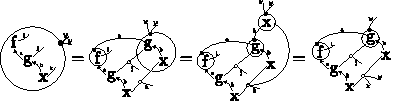
\includegraphics[width=.8\textwidth]{figures/chain_rule_broadcast.pdf}
\]

\subsection{Functions with multiple inputs}
If $f : \mathbb{R}^m \times \mathbb{R}^n \to \mathbb{R}$ is a function with two inputs, the derivative of $f(x,y)$ is simply $\frac{\partial f}{\partial x}\partial x + \frac{\partial f}{\partial y}\partial y$,
or in tensor diagram notation:
\[
   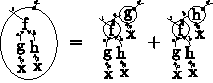
\includegraphics[width=.45\textwidth]{figures/multi_input_functions.pdf}
\]

\section{Examples}

\subsection{Known derivatives}
Two examples where we can expand \tikz[baseline=(f.base), inner sep=2pt]{\node[dn](f){$f$}; \draw[d0](f)--++(.6,0);} with known derivatives:
\[
   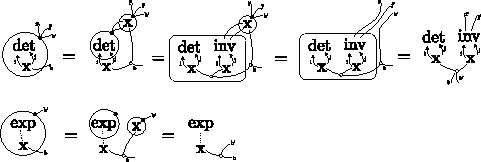
\includegraphics[width=\textwidth]{figures/other_functions.pdf}
\]
Here $\mathrm{inv}(X)$ is the matrix inverse function, taking a matrix $X$ to its inverse $X^{-1}$.
In the case of the determinant, one may continue taking derivatives to find the
simple pattern
\[
   \frac{\partial^k \det(X)}{\partial X^k} = \det(X) (X^{-1})^{\otimes k}.
\]


\subsection{Pseudo-linear forms}

Pseudo-linear forms, $A(x)x$, are common.
All pixel-adaptive filters like non-local means, bilateral, etc, and the so-called attention mechanism in transformers can be written this way.
According to Peyman Milanfar, the gradient of this function is important and has a form worth remembering:
\[
   \begin{tikzpicture}[baseline=-1em, inner sep=1pt]
      \node (n0) {$A$};
      \node[below=1em of n0] (n1) {$x$};
      \node[right=1em of n0] (n2) {$x$};
      \draw[->] (n1) -- (n0);
      \draw (n2) -- (n0);
      \drawellipse{.25}{-.25}{.7}{.7}{180/4}
      \draw (n0) -- ++(-.5,0);
   \end{tikzpicture}
   =
   \hspace{.5em}
   \begin{tikzpicture}[baseline=-1em, inner sep=1pt]
      \node (n0) {$A$};
      \node[below=1em of n0] (n1) {$x$};
      \node[right=1em of n0] (n3) {$x$};
      \draw[->] (n1) -- (n0);
      \draw (n0) -- (n3);
      \drawellipse{0}{-.25}{.4}{.7}{180/4}
      \draw (n0) -- ++(-.5,0);
   \end{tikzpicture}
   +
   \hspace{.5em}
   \begin{tikzpicture}[baseline=-1em, inner sep=1pt]
      \node (n0) {$A$};
      \node[below=1em of n0] (n1) {$x$};
      \node[right=.75em of n0] (n3) {$x$};
      \draw[->] (n1) -- (n0);
      \draw (n0) -- (n3);
      \draw (n0) -- ++(-.5,0);
      \drawellipse{.575}{0}{.25}{.25}{180/4}
   \end{tikzpicture}
   =
   \hspace{.5em}
   \begin{tikzpicture}[baseline=-1em, inner sep=1pt]
      \node[dn] (n0) {$A$};
      \node[below=1em of n0] (n1) {$x$};
      \node[right=.75em of n0] (n3) {$x$};
      \draw[->] (n1) -- (n0);
      \draw (n0) -- (n3);
      \draw[d0] (n0) -- ++(.4,.4);
      \draw (n0) -- ++(-.5,0);
   \end{tikzpicture}
   +
   \hspace{.5em}
   \begin{tikzpicture}[baseline=-1em, inner sep=1pt]
      \node (n0) {$A$};
      \node[below=1em of n0] (n1) {$x$};
      \draw[->] (n1) -- (n0);
      \draw (n0) -- ++(.5,0);
      \draw (n0) -- ++(-.5,0);
   \end{tikzpicture}
\]
We may appreciate the simplicity of this expression, when we consider the following derivation given by Peyman Milanfar using classical notation:
\begin{align*}
   \mathrm{d}[A(x) x]
   & =\mathrm{d}[A(x)] x+A(x) \mathrm{d} x 
   \\& =\operatorname{vec}{\mathrm{d}[A(x)] x}+A(x) \mathrm{d} x 
   \\& =\operatorname{vec}{I \mathrm{d}[A(x)] x}+A(x) \mathrm{d} x 
   \\& =(x^T \otimes I) \operatorname{vec}{\mathrm{d}[A(x)]}+A(x) \mathrm{d} x 
   \\& =(x^T \otimes I) \mathrm{D} \operatorname{vec}[A(x)] \mathrm{d} x+A(x) \mathrm{d} x 
   \\& =[(x^T \otimes I) \mathrm{D} \operatorname{vec}[A(x)]+A(x)] \mathrm{d} x
\end{align*}
Which finally implies:
\begin{align*}
\hspace{-2em}
   \frac{\partial A(x)x}{\partial x}
   &= (x^T \otimes I) \frac{\partial}{\partial x}  \mathrm{vec}[A(x)] + A(x)
   .
\end{align*}

\subsection{Trace identity}
The Matrix Cookbook has the formula:
\begin{align}
   \tag{128}
   \frac{\partial \Tr(\sin(x))}{\partial x}
   &= \cos(x)^T
\end{align}
If we attempt to derive this using tensor diagrams, we get the following different result,
\[
   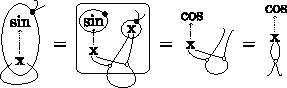
\includegraphics[width=.5\textwidth]{figures/cos.pdf}
\]
which is equivalent to $\cos(x) \circ I$.
That is, $\cos(x)$ but zero everywhere except the diagonal.

The reason is that the matrix cookbook actually uses a slightly different definition of ``function applied to matrix''.
If $F$ can be written as a power series, then one way to define $F(X)$ is the matrix power series:
\[
   F(X) = \sum_{k=0}^\infty a_k X^k.
\]
In this case, the derivative of $\Tr(F(X))$ is
$f(X)^T$, where $f(X)$ is the scalar derivative of $F(X)$,
matching the Matrix Cookbook's formula.


\subsection{Taylor}
For an n-times differentiable function $v: \R^d\to\R^d$ we can write the Taylor expansion:
\[
   \begin{tikzpicture}[baseline=-1em, inner sep=1pt]
      \node (n0) {$v$};
      \node[below=1em of n0] (n1) {$(x+\eps)$};
      \draw[->] (n1) -- (n0);
      \draw (n0) -- ++(.5,0);
   \end{tikzpicture}
   \approx
   \begin{tikzpicture}[baseline=-1em, inner sep=1pt]
      \node (n0) {$v$};
      \node[below=1em of n0] (n1) {$x$};
      \draw[->] (n1) -- (n0);
      \draw (n0) -- ++(.5,0);
   \end{tikzpicture}
   +
   \begin{tikzpicture}[baseline=-1em, inner sep=1pt]
      \node[dn] (n0) {$v$};
      \node[below=1em of n0] (n1) {$x$};
      \node[left=1em of n0] (n2) {$\eps$};
      \draw[->] (n1) -- (n0);
      \draw[d0] (n0) -- (n2);
      \draw (n0) -- ++(.5,0);
   \end{tikzpicture}
   +\frac12
   %\hspace{.5em}
   \begin{tikzpicture}[baseline=-1em, inner sep=1pt]
      \node[ddn] (n0) {$v$};
      \node[below=1em of n0] (n1) {$x$};
      \node[left=1em of n0] (n2) {$\eps$};
      \node[left=.75em of n0, yshift=-1em] (n3) {$\eps$};
      \draw[->] (n1) -- (n0);
      \draw[d0] (n0) -- (n2);
      \draw[d0] (n0) -- (n3);
      \draw (n0) -- ++(.5,0);
   \end{tikzpicture}
   +
   \frac16
   %\hspace{.5em}
   \begin{tikzpicture}[baseline=-1em, inner sep=1pt]
      \node[dddn] (n0) {$v$};
      \node[below=1em of n0] (n1) {$x$};
      \node[left=1em of n0] (n2) {$\eps$};
      \node[left=.75em of n0, yshift=-1em] (n3) {$\eps$};
      \node[left=.75em of n0, yshift=1em] (n4) {$\eps$};
      \draw[->] (n1) -- (n0);
      \draw[d0] (n0) -- (n2);
      \draw[d0] (n0) -- (n3);
      \draw[d0] (n0) -- (n4);
      \draw (n0) -- ++(.5,0);
   \end{tikzpicture}
   +
   \dots
\]

Writing this using classical notation is quite messy:
\begin{align*}
    v(x + \eps)
    &\approx
    v(x)
    + \left[\frac{\partial}{\partial x} v(x)\right]\eps
    + \frac{1}{2}\left[\frac{\partial}{\partial x}\left[\frac{\partial}{\partial x} v(x)\right]\eps\right]\eps
    + \frac{1}{6}\left[\frac{\partial}{\partial x}\left[\frac{\partial}{\partial x} \left[\frac{\partial}{\partial x} v(x)\right]\eps\right]\eps\right]\eps
    + \dots
    \\
    &=
    v(x)
    + \left[\frac{\partial}{\partial x} v(x)\right]\eps
    +
    \frac{1}{2}
    (I \otimes \eps)
    \left[\frac{\partial\mathrm{vec}}{\partial x}\left[\frac{\partial v(x)}{\partial x} \right]\right]\eps
    + \frac{1}{6}
    (I \otimes \eps \otimes \eps)
    \left[\frac{\partial\mathrm{vec}}{\partial x}\left[\frac{\partial\mathrm{vec}}{\partial x} \left[\frac{\partial v(x)}{\partial x} \right]\right]\right]\eps
    + \dots
\end{align*}
With index notation it's ok:
\begin{align*}
    v_i(x + \eps)
    &\approx
    v_i(x)
    + \sum_j \frac{\partial v_i(x)}{\partial x_j} \eps_j
    + \frac12 \sum_{j,k} \frac{\partial^2 v_i(x)}{\partial x_j\partial x_k} \eps_j \eps_k
   + \frac16 \sum_{j,k,\ell} \frac{\partial^3 v_i(x)}{\partial x_j\partial x_k\partial x_\ell} \eps_j \eps_k \eps_\ell
\end{align*}
% TODO: Examples based on idempotent matrices etc.



\section{Exercises}
\begin{exercise}
   Draw the tensor diagram for a function $f:\mathbb{R}^n\to\mathbb{R}$ that applies an element-wise nonlinearity (for instance, $\exp$) followed by a summation over the components. Verify that the diagram corresponds to the conventional formula for the softmax denominator.
\end{exercise}

\begin{exercise}
   Represent the composition of two functions 
   \[
      f:\mathbb{R}^m\to\mathbb{R} \quad \text{and} \quad v:\mathbb{R}^n\to\mathbb{R}^m,
   \]
   using tensor diagrams. Then, using the diagrammatic chain rule, derive the expression for the derivative of $f\circ v$ with respect to $x\in\mathbb{R}^n$.
\end{exercise}

\begin{exercise}
   For a matrix function $A(x)$ that depends on a vector $x$, use tensor diagrams to illustrate the derivative 
   \[
      \frac{\partial}{\partial x}[A(x)x],
   \]
   and explain how the product rule is implemented in the diagram.
\end{exercise}

\begin{exercise}
   % Source: Adapted from StackExchange VAE backpropagation questions (e.g., by greg).
   % Answer: Using the chain rule and elementwise differentiation, one obtains 
   % $\nabla_W KL = \frac{1}{2}\Big(e^{Wx+c} - 1\Big)x^T$, where the exponential is applied elementwise.
   Represent the KL-divergence term for a Variational Autoencoder (VAE) as
   \[
      KL(\mu,\sigma) = -\frac{1}{2}\Big(1 + \log\sigma^2 - \mu^2 - \sigma^2\Big),
   \]
   with parameters given by 
   \[
      \mu = W x + c \quad \text{and} \quad \log\sigma^2 = W x + c.
   \]
   Derive the gradient $\nabla_W KL$ with respect to the weight matrix $W$. Be sure to keep track of dimensions and account for elementwise operations.
\end{exercise}
\begin{exercise}
   % Source: A well-known result in machine learning; see many SE posts (e.g., greg's answers).
   % Answer: The Jacobian is given by 
   % $\displaystyle \frac{\partial s_i}{\partial z_j} = s_i\big(\delta_{ij} - s_j\big)$.
   Let the softmax function $s:\mathbb{R}^n \to \mathbb{R}^n$ be defined by
   \[
      s_i(z) = \frac{e^{z_i}}{\sum_{j=1}^n e^{z_j}}, \quad i=1,\dots,n.
   \]
   Prove that the Jacobian matrix of $s$ is given by
   \[
      \frac{\partial s_i}{\partial z_j} = s_i\big(\delta_{ij} - s_j\big),
   \]
   where $\delta_{ij}$ is the Kronecker delta.
\end{exercise}

\begin{exercise}
   % Source: Standard derivations found in textbooks and the Matrix Cookbook.
   % Answer: Differentiation yields $\nabla_\mu \ell = \Sigma^{-1}\sum_{i}(x^{(i)}-\mu)$ and 
   % $\nabla_\Sigma \ell = -\frac{n}{2}\Sigma^{-1} + \frac{1}{2}\Sigma^{-1}S\Sigma^{-1}$; setting these to zero leads to 
   % $\hat\mu = \frac{1}{n}\sum_{i=1}^n x^{(i)}$ and $\hat\Sigma = \frac{1}{n}\sum_{i=1}^n (x^{(i)}-\hat\mu)(x^{(i)}-\hat\mu)^T$.
   Suppose $x^{(1)},\dots,x^{(n)} \in \mathbb{R}^d$ are independent samples from a multivariate normal distribution $N(\mu,\Sigma)$. Write the log-likelihood function and derive the gradients $\nabla_\mu \ell$ and $\nabla_\Sigma \ell$. Then, by setting these gradients to zero, show that the maximum likelihood estimators are
   \[
      \hat\mu = \frac{1}{n}\sum_{i=1}^n x^{(i)} \quad \text{and} \quad \hat\Sigma = \frac{1}{n}\sum_{i=1}^n (x^{(i)} - \hat\mu)(x^{(i)} - \hat\mu)^T.
   \]
\end{exercise}

\begin{exercise}
   % Source: Derived from Gaussian process literature and related SE discussions.
   % Answer: The derivative is 
   % $\displaystyle \frac{\partial L}{\partial \theta} = \frac{1}{2}\operatorname{tr}\!\Big(\Big(K^{-1}yy^T K^{-1} - K^{-1}\Big)\frac{\partial K}{\partial \theta}\Big)$.
   Consider a Gaussian process with covariance matrix $K(\theta)$ and the log-marginal likelihood defined as
   \[
      L(\theta) = -\frac{1}{2}\Big(y^T K(\theta)^{-1} y + \log\det K(\theta)\Big).
   \]
   Derive the gradient of $L$ with respect to $\theta$, showing that
   \[
      \frac{\partial L}{\partial \theta} = \frac{1}{2}\operatorname{tr}\!\Big(\Big(K^{-1}yy^T K^{-1} - K^{-1}\Big)\frac{\partial K}{\partial \theta}\Big).
   \]
\end{exercise}

\begin{exercise}
   % Source: Standard logistic regression derivations and multiple SE posts.
   % Answer: One obtains $\nabla_w J = \sum_{i=1}^n (p_i - y_i)x_i$ and the Hessian 
   % $H = \sum_{i=1}^n p_i(1-p_i)x_i x_i^T$.
   In logistic regression, let 
   \[
      p_i = \sigma(w^T x_i) \quad \text{with} \quad \sigma(z)=\frac{1}{1+e^{-z}},
   \]
   and consider the negative log-likelihood
   \[
      J(w) = -\sum_{i=1}^n \Big[y_i\ln p_i + (1-y_i)\ln(1-p_i)\Big].
   \]
   Derive the gradient $\nabla_w J$ and the Hessian $H = \nabla^2_w J$. In particular, show that
   \[
      \nabla_w J = \sum_{i=1}^n (p_i - y_i)x_i, \quad \text{and} \quad H = \sum_{i=1}^n p_i(1-p_i)\,x_i x_i^T.
   \]
\end{exercise}

\begin{exercise}
   % Source: Matrix Cookbook and classic derivations in matrix calculus.
   % Answer: The derivative is $\nabla_X \det(X) = \det(X)\,(X^{-1})^T$.
   Let $X \in \mathbb{R}^{n\times n}$ be an invertible matrix. Prove that
   \[
      \frac{\partial\,\det(X)}{\partial X} = \det(X)\,(X^{-1})^T.
   \]
   In other words, show that the gradient of $\det(X)$ with respect to $X$ is $\det(X)$ times the transpose of $X^{-1}$.
\end{exercise}

\begin{exercise}
   % Source: Standard result from the Matrix Cookbook.
   % Answer: $\nabla_X \ln\det(X) = (X^{-1})^T$.
   For an invertible matrix $X \in \mathbb{R}^{n\times n}$, prove that
   \[
      \frac{\partial}{\partial X}\ln\det(X) = (X^{-1})^T.
   \]
   Briefly discuss why this result is useful in statistical applications such as Gaussian likelihoods.
\end{exercise}

\begin{exercise}
   % Source: Matrix Cookbook and related SE discussions.
   % Answer: By differentiating $I = A^{-1}A$, we find 
   % $d(A^{-1}) = -A^{-1}(dA)A^{-1}$.
   Let $A \in \mathbb{R}^{n\times n}$ be an invertible matrix (which may depend on a parameter). Starting from the identity $I = A^{-1}A$, differentiate both sides to show that
   \[
      d(A^{-1}) = -A^{-1}\,(dA)\,A^{-1}.
   \]
   Deduce an expression for the partial derivative $\frac{\partial A^{-1}}{\partial A_{ij}}$.
\end{exercise}

\begin{exercise}
   % Source: Derived from the differentiation of an inverse matrix (see Matrix Cookbook).
   % Answer: The gradient is given by 
   % $\nabla_A f(A) = -A^{-T}(a\,b^T)A^{-T}$.
   Define the scalar function
   \[
      f(A)=a^T A^{-1} b,
   \]
   where $a,b\in\mathbb{R}^n$ are fixed vectors and $A\in\mathbb{R}^{n\times n}$ is invertible. Using the result from differentiating the inverse, show that
   \[
      \nabla_A f(A) = -A^{-T}(a\,b^T)A^{-T}.
   \]
\end{exercise}

\begin{exercise}
   % Source: A classical perturbation result found in textbooks and SE posts.
   % Answer: For a simple eigenvalue $\lambda$ with unit eigenvector $v$, 
   % $\nabla_X \lambda = v\,v^T$. This result does not hold when $\lambda$ is multiple.
   Let $X\in\mathbb{R}^{n\times n}$ be a symmetric matrix with a simple eigenvalue $\lambda$ and corresponding unit eigenvector $v$. Prove that the derivative of $\lambda$ with respect to $X$ is given by
   \[
      \nabla_X \lambda = v\,v^T.
   \]
   Additionally, discuss why this result does not hold when $\lambda$ has multiplicity greater than one.
\end{exercise}

\begin{exercise}
   % Source: Classical result using Lagrange multipliers; see standard textbooks.
   % Answer: The stationary condition yields $Ax = \lambda x$, so the extrema of the Rayleigh quotient are the eigenvalues of $A$, with the maximizer (minimizer) corresponding to the largest (smallest) eigenvalue.
   For a symmetric matrix $A\in\mathbb{R}^{n\times n}$, consider the Rayleigh quotient
   \[
      R(x) = \frac{x^T A x}{x^T x}, \quad x\in\mathbb{R}^n\setminus\{0\}.
   \]
   Using Lagrange multipliers, show that the stationary values of $R(x)$ correspond to the eigenvalues of $A$, and that the maximizer (minimizer) is the eigenvector associated with the largest (smallest) eigenvalue.
\end{exercise}
\begin{exercise}
   % Source: Matrix Cookbook and common SE answers.
   % Answer: The derivative is 
   % $\nabla_X\,\operatorname{Tr}(X^T A X B) = A X B^T + A^T X B$.
   Let $A\in\mathbb{R}^{m\times m}$ and $B\in\mathbb{R}^{n\times n}$ be constant matrices, and let $X\in\mathbb{R}^{m\times n}$ be a variable matrix. Prove that
   \[
      \nabla_X\,\operatorname{Tr}(X^T A X B) = A X B^T + A^T X B.
   \]
   (Hint: Use the cyclic property of the trace to rearrange terms.)
\end{exercise}

\begin{exercise}
   % Source: Direct differentiation of trace forms; see also the Matrix Cookbook.
   % Answer: (a) $\frac{\partial}{\partial X} \operatorname{Tr}(A^T X) = A$, (b) $\nabla_X\,\operatorname{Tr}(A X B) = A^T B^T$.
   \textbf{(a)} Show that for a constant matrix $A\in\mathbb{R}^{m\times n}$ and variable $X\in\mathbb{R}^{m\times n}$,
   \[
      \frac{\partial}{\partial X} \operatorname{Tr}(A^T X) = A.
   \]
   \textbf{(b)} More generally, for constant matrices $A\in\mathbb{R}^{p\times m}$ and $B\in\mathbb{R}^{n\times q}$, prove that
   \[
      \nabla_X\,\operatorname{Tr}(A X B) = A^T B^T.
   \]
\end{exercise}

\begin{exercise}
   % Source: Inspired by tensor diagram techniques and SE discussions.
   % Answer: By differentiating $F(s)=\Diag(s)C\Diag(s)$, one obtains 
   % $dF = \Diag(ds)C\,\Diag(s) + \Diag(s)C\,\Diag(ds)$, leading to 
   % $\nabla_s F(s)$ that relates (after suitable vectorization) to $2\,\Diag(C\,s)$.
   Let $s\in\mathbb{R}^n$ be a vector and $C\in\mathbb{R}^{n\times n}$ be a fixed matrix. Define the matrix function 
   \[
      F(s) = \diag(s)\,C\,\diag(s),
   \]
   where $\diag(s)$ denotes the diagonal matrix with the entries of $s$. Express the differential $dF$ in terms of $s$, $ds$, and $C$, and hence derive an expression for the derivative $\nabla_s F(s)$.
\end{exercise}

\begin{exercise}
   % Source: Standard vectorization identities from the Matrix Cookbook.
   % Answer: The identity is 
   % $\operatorname{vec}(A\,X\,B^T) = (B \otimes A)\,\operatorname{vec}(X)$.
   Let $A\in\mathbb{R}^{p\times m}$, $X\in\mathbb{R}^{m\times n}$, and $B\in\mathbb{R}^{n\times q}$. Prove the identity
   \[
      \operatorname{vec}(A\,X\,B^T) = (B \otimes A)\,\operatorname{vec}(X).
   \]
   Discuss how this identity can be used to convert certain matrix derivative problems into vectorized forms.
\end{exercise}
\begin{exercise}
   % Source: Standard differentiation of quadratic forms.
   % Answer: The gradient is $\nabla_x f(x) = (A+A^T)x$, and the Hessian is $\nabla^2_x f(x) = A+A^T$. For symmetric $A$, this simplifies to $2A$.
   Let 
   \[
      f(x) = x^T A x,
   \]
   where $x\in\mathbb{R}^n$ and $A\in\mathbb{R}^{n\times n}$ is not necessarily symmetric. Show that
   \[
      \nabla_x f(x) = (A + A^T)x.
   \]
   Then, compute the Hessian $\nabla^2_x f(x)$ and discuss what simplification occurs when $A$ is symmetric.
\end{exercise}
\begin{exercise}
   % Source: Standard convex analysis and properties of the Frobenius norm.
   % Answer: For $X\neq 0$, $\nabla_X \|X\|_F = \frac{X}{\|X\|_F}$. At $X=0$, the gradient is not unique; any matrix $G$ with $\|G\|_F\le 1$ is a subgradient.
   Consider the Frobenius norm
   \(
      \|X\|_F = \sqrt{\operatorname{Tr}(X^T X)},
   \)
   for $X\in\mathbb{R}^{m\times n}$.

   Show that
   \[
      \nabla_X \|X\|_F = \frac{X}{\|X\|_F}
   \]
   for $X\neq 0$.
\end{exercise}
\begin{exercise}
   % Source: Based on discussions of spectral function differentiability on SE.
   % Answer: When the largest eigenvalue has multiplicity $k>1$, any matrix of the form 
   % $G = \sum_{i=1}^k u_i v_i^T$, where $\{u_i\}$ is an orthonormal basis for the eigenspace, is a valid subgradient. The gradient is not unique in this case.
   Let $Y\in\mathbb{R}^{n\times n}$ be a symmetric matrix, and define $\phi(Y)$ to be its largest eigenvalue. If this eigenvalue has multiplicity $k>1$, show that the derivative of $\phi(Y)$ is not unique. In particular, demonstrate that any matrix of the form
   \[
      G = \sum_{i=1}^k u_i v_i^T,
   \]
   where $\{u_i\}_{i=1}^k$ is any orthonormal basis for the eigenspace corresponding to the largest eigenvalue, is a valid subgradient of $\phi(Y)$. Explain the challenges that arise in defining a unique gradient in this setting.
\end{exercise}


\chapter{Statistics and Probability}
\section{Definition of Moments}
Let $x\in\mathbb R^{n}$ is a random variable.
We write $m = E[x]\in\mathbb R^n$ for the expectation and
$M=\mathrm{Var}[x] = E[(x-m)(x-m)^T]$ for the covariance (when these quantities are defined.)

In tensor diagrams, we will use square brackets:
\[
   \vecmatvec{1em}{}{}{m}
   =
\mathbin{\begin{tikzpicture}[baseline=(n0.base), inner sep=1pt]
   \node (n0) at (0,0) {$[$};
   \node [right=1em of n0] (n1) {$x]$};
   \draw (n0) -- (n1);
\end{tikzpicture}}
\quad\text{and}\quad
   \vecmatvec{1em}{}{M}{}
   =
\mathbin{\begin{tikzpicture}[baseline=(n0.base), inner sep=1pt]
   \node (n0) at (0,0) {$[$};
   \node [right=1em of n0] (n1) {$(x\ominus m)$};
   \node [right=.5em of n1] (n2) {$(x\ominus m)$};
   \node [right=1em of n2] (n3) {$]$};
   \draw (n0) -- (n1);
   \draw (n2) -- (n3);
\end{tikzpicture}}
\]
We will use the circled minus, $\ominus$, to distinguish the operation from contraction edges.

We can also define the third and fourth centralized moment tensors
\[
   \begin{tikzpicture}[baseline=(T.base), inner sep=1pt]
      \node (T) {$M_3$};
      \draw (T) -- ++(.5,.3);
      \draw (T) -- ++(.5,-.3);
      \draw (T) -- ++(.5,0);
   \end{tikzpicture}
   =
   \renewcommand*{\arraystretch}{1.3}
   \begin{bmatrix}
      \vecmatvec{1em}{(x\ominus m)}{}{} \\
      \vecmatvec{1em}{(x\ominus m)}{}{} \\
      \vecmatvec{1em}{(x\ominus m)}{}{}
   \end{bmatrix}
\quad\text{and}\quad
   \begin{tikzpicture}[baseline=(T.base), inner sep=1pt]
      \node (T) {$M_4$};
      \draw (T) -- ++(.5,.5);
      \draw (T) -- ++(.5,-.5);
      \draw (T) -- ++(.5,.2);
      \draw (T) -- ++(.5,-.2);
   \end{tikzpicture}
   =
   \renewcommand*{\arraystretch}{1.3}
   \begin{bmatrix}
      \vecmatvec{1em}{(x\ominus m)}{}{} \\
      \vecmatvec{1em}{(x\ominus m)}{}{} \\
      \vecmatvec{1em}{(x\ominus m)}{}{} \\
      \vecmatvec{1em}{(x\ominus m)}{}{}
   \end{bmatrix}
.
\]
%These are less common in introductory causes, even though the scalar third and fourth moment are common.
%This is presumably because they require higher order tensors.

%If the entries of $x$ are independent, the non-diagonal entries disappear, so we get
%\[
%M =
%\left[
%   \begin{tikzpicture}[baseline=(c.base), inner sep=1pt]
%      \node (T1) {$(x\ominus m)$};
%      \node (T2)[below=.5em of T1] {$(x\ominus m)$};
%      \node (c)[right=.7em of T1, yshift=-1em] {$\sbullet$};
%      \draw (T1) -- (c);
%      \draw (T2) -- (c);
%      \draw (c) -- ++(.7em,0);
%   \end{tikzpicture}
%\right]
%\quad\text{and}\quad
%M_3 =
%\left[
%   \begin{tikzpicture}[baseline=(T2.base), inner sep=1pt]
%      \node (T1) {$(x\ominus m)$};
%      \node (T2)[below=.5em of T1] {$(x\ominus m)$};
%      \node (T3)[below=.5em of T2] {$(x\ominus m)$};
%      \node (c)[right=.7em of T2] {$\sbullet$};
%      \draw (T1) -- (c);
%      \draw (T2) -- (c);
%      \draw (T3) -- (c);
%      \draw (c) -- ++(.7em,0);
%   \end{tikzpicture}
%\right]
%\quad\text{and so on.}
%\]
% If the entries are also identically distributed, we simply have
% \[
%    M = \sigma^2
%    \,
% \begin{tikzpicture}[baseline=(T.base), inner sep=0]
%    \node (T) {$\sbullet$};
%    \draw (T) -- ++(0,.3);
%    \draw (T) -- ++(0,-.3);
% \end{tikzpicture}
%    \text{ and }
%    M_3 = \mathrm{E}[(x_0-m_0)^3]
% \begin{tikzpicture}[baseline=(T.base), inner sep=0]
%    \node (T) {$\sbullet$};
%    \draw (T) -- ++(0,.3);
%    \draw (T) -- ++(-.2,-.3);
%    \draw (T) -- ++(.2,-.3);
% \end{tikzpicture}
% .
% \]


\subsection{Expectation of Linear Combinations}
General principle: The ``linearity of expectation'' lets you pull out all parts of the graph not involving $X$.
\[
   \vcenter{\hbox{
      \import{figures/}{linearityOfExpectation.pdf_tex}
   }}
\]
where $M_3$ is the expectation\footnote{FIXME: This is different from the notation just introduced above.}
\(
\left[
\begin{tikzpicture}[baseline=(T.base), inner sep=1pt]
   \node (T) {$x$};
   \draw (T) -- ++(0,.3);
   \draw (T) -- ++(-.1,-.3);
   \draw (T) -- ++(.1,-.3);
\end{tikzpicture}
\,
\begin{tikzpicture}[baseline=(T.base), inner sep=1pt]
   \node (T) {$x$};
   \draw (T) -- ++(0,.3);
   \draw (T) -- ++(-.1,-.3);
   \draw (T) -- ++(.1,-.3);
\end{tikzpicture}
\,
\begin{tikzpicture}[baseline=(T.base), inner sep=1pt]
   \node (T) {$x$};
   \draw (T) -- ++(0,.3);
   \draw (T) -- ++(-.1,-.3);
   \draw (T) -- ++(.1,-.3);
\end{tikzpicture}
\right]
\),
which is an order-9 tensor with no dependence on the constants $A$, $B$, $C$ and $D$.
In practice you would want to name the edges to keep track of what gets multiplied with what.

We can even use linearity of expectation to push the expectation inside an infinite sum of tensors, as in the following moment generating function, which relates all the $M_k$ tensors:
\begin{align*}
   \mathrm{E}(\mathrm{e}^{\langle x\ominus m, t\rangle})
   &= \sum_{k=0}^\infty \frac{1}{k!} \mathrm{E}[\langle x\ominus m, t\rangle^k]
    = \mathrm{E}\big[\sum_{k=0}^\infty \frac{1}{k!} \langle (x\ominus m)^{\otimes k}, t^{\otimes k}\rangle\big]
   = \sum_{k=0}^\infty \frac{1}{k!} \langle M_k, t^{\otimes k}\rangle
 \\&=
  % =
   1
   +
   \begin{tikzpicture}[baseline=.5em, inner sep=1]
      \node (T) {$m$};
      \draw (T) -- ++(0,.5) node[fill=white] {$t$};
   \end{tikzpicture}
   +
   \frac{1}{2}
   \begin{tikzpicture}[baseline=(T.base), inner sep=1]
      \node (T) {$M$};
      \draw (T) -- ++(0,.5) node[fill=white] {$t$};
      \draw (T) -- ++(0,-.5) node[fill=white] {$t$};
   \end{tikzpicture}
   +
   \frac{1}{6}
   \begin{tikzpicture}[baseline=(T.base), inner sep=1]
      \node (T) {$M_3$};
      \draw (T) -- ++(0,.5) node[fill=white] {$t$};
      \draw (T) -- ++(-.4,-.4) node[fill=white] {$t$};
      \draw (T) -- ++(.4,-.4) node[fill=white] {$t$};
   \end{tikzpicture}
   +
   \frac{1}{24}
   \begin{tikzpicture}[baseline=(T.base), inner sep=1]
      \node (T) {$M_4$};
      \draw (T) -- ++(-.4,-.4) node[fill=white] {$t$};
      \draw (T) -- ++(.4,-.4) node[fill=white] {$t$};
      \draw (T) -- ++(-.4,.4) node[fill=white] {$t$};
      \draw (T) -- ++(.4,.4) node[fill=white] {$t$};
   \end{tikzpicture}
   +
   \dots
\end{align*}

\subsection{Linear Forms}
The Matrix Cookbook gives the following simple expectation:
\begin{walign}
   \tag{312}
   \E[AXB+C] &= A \E[X] B + C
   &
   \renewcommand*{\arraystretch}{1.3}
   \begin{bmatrix}
      \matmul{A,X,B} \\+\, \matmul{C}
   \end{bmatrix}
   &=
   \renewcommand*{\arraystretch}{1.3}
   \begin{matrix}
      \matmul{A,[X],B} \\+\, \matmul{C}
   \end{matrix}
\end{walign}

\subsection{Quadratic Forms}
We often prefer to write expectations in terms of the simple centered moments, which we can do by pulling out the mean:
\renewcommand*{\arraystretch}{1}
\[
   \begin{bmatrix}
      x - \\
      x -
   \end{bmatrix}
   =
   \begin{bmatrix}
      (x\ominus m) - \\
      (x\ominus m) -
   \end{bmatrix}
   +
   \begin{array}{c}
      m - \\
      m -
   \end{array}
   =
   \begin{tikzpicture}[baseline=(T.base), inner sep=1pt]
      \node (T) {$M$};
      \draw (T) -- ++(.5,.25);
      \draw (T) -- ++(.5,-.25);
   \end{tikzpicture}
   +
   \begin{array}{c}
      m - \\
      m -
   \end{array}
\]
This makes it easy to handle the quadratic forms from the Matrix Cookbook:
\begin{walign}
   \tag{313}
   \mathrm{Var}[Ax] &= A \mathrm{Var}[x] A^T
   &
   \renewcommand*{\arraystretch}{1.3}
   \begin{bmatrix}
      \vecmatvec{.5em}{A}{}{x} \ominus [\vecmatvec{.5em}{A}{}{x}] \\
      \vecmatvec{.5em}{A}{}{x} \ominus [\vecmatvec{.5em}{A}{}{x}]
   \end{bmatrix}
   &=
   \renewcommand*{\arraystretch}{1.3}
   \begin{bmatrix}
      \vecmatvec{.5em}{A}{}{(x\ominus m)} \\
      \vecmatvec{.5em}{A}{}{(x\ominus m)}
   \end{bmatrix}
 \\&&&=
   \vcenter{\hbox{\begin{tikzpicture}[inner sep=1pt]
      \node (n1) at (0,-.25) {$\vecmatvec{1em}{A}{}{(x\ominus m)}$};
      \node (n2) at (0,.25) {$\vecmatvec{1em}{A}{}{(x\ominus m)}$};
      \node at (-.45, 0) {$\Bigg[$};
      \node at (1, 0) {$\Bigg]$};
   \end{tikzpicture}}}
 \\&&& =
   \vecmatvec{.5em}{}{A,M_2,A}{}
%%%%%%%%%%%%%%%%%%%%%%%%%%%%%%%%%%%%%%%%%%%%%%%%%%%%%%%%%%%%%%%%%%%%%%%%%%%%%%%%
   \\[.5em]
   \tag{318}
   \E[x^T A x]
   &= \mathrm{Tr}(A M) + m^T A m
   &
   [\vecmatvec{.5em}{x}{A}{x}]
   &=
   \left(
      \begin{bmatrix}
         (x\ominus m) - \\
         (x\ominus m) -
      \end{bmatrix}
      +
      \begin{array}{c}
         m - \\
         m -
      \end{array}
   \right)
   \begin{tikzpicture}[baseline=(A.base), inner sep=1pt]
      \node (A) {$A$};
      \draw (A) -- ++(-.5, .1);
      \draw (A) -- ++(-.5, -.1);
   \end{tikzpicture}
   \\
   &&&=
   \mathbin{\begin{tikzpicture}[baseline=(A.base), inner sep=1pt]
      \node (n1) at (0,-.25) {$(x\ominus m)$};
      \node (n2) at (0,.25) {$(x\ominus m)$};
      \node at (-.75, 0) {$\Bigg[$};
      \node at (.75, 0) {$\Bigg]$};
      \node (A) at (1, 0) {$A$};
      \draw (n1) -- (A);
      \draw (n2) -- (A);
   \end{tikzpicture}}
   +
   \begin{tikzpicture}[baseline=(A.base), inner sep=1pt]
      \node (A) {$A$};
      \node (m1) at (-.75, .2) {$m$};
      \node (m2) at (-.75, -.2) {$m$};
      \draw (m1) -- (A) -- (m2);
   \end{tikzpicture}
   \\
   &&&=
   \trace{M,A}2
   +
   \vecmatvec{.5em}{m}{A}{m}
   \\[.5em]
\end{walign}

\begin{align*}
   E[(A\mathbf{x} + a)(B\mathbf{x} + b)^T] &= AMB^T + (Am + a)(Bm + b)^T \tag{320} \\
   E[\mathbf{x}\mathbf{x}^T] &= M + mm^T \tag{321} \\
   E[\mathbf{x} a^T \mathbf{x}] &= (M + mm^T)a \tag{322} \\
   E[\mathbf{x}^T a\mathbf{x}^T] &= a^T(M + mm^T) \tag{323} \\
   E[(A\mathbf{x})(A\mathbf{x})^T] &= A(M + mm^T)A^T \tag{324} \\
   E[(\mathbf{x} + a)(\mathbf{x} + a)^T] &= M + (m + a)(m + a)^T \tag{325} \\
   E[(A\mathbf{x} + a)^T(B\mathbf{x} + b)] &= \text{Tr}(AMB^T) + (Am + a)^T(Bm + b) \tag{326} \\
   E[\mathbf{x}^T \mathbf{x}] &= \text{Tr}(M) + m^T m \tag{327} \\
   E[\mathbf{x}^T A\mathbf{x}] &= \text{Tr}(AM) + m^T Am \tag{328} \\
   E[(A\mathbf{x})^T(A\mathbf{x})] &= \text{Tr}(AMA^T) + (Am)^T(Am) \tag{329} \\
   E[(\mathbf{x} + a)^T(\mathbf{x} + a)] &= \text{Tr}(M) + (m + a)^T(m + a) \tag{330}
\end{align*}



\subsection{Cubic Forms}

\[
\begin{tikzpicture}[scale=1.3,
  every node/.style={inner sep=1pt, circle, draw, fill=white, thin},
  label/.style={draw=none, fill=none, text=black, font=\scriptsize},
  declare function={
    xgap=.8;  % Horizontal spacing between diagrams
  }]

  \drawPartitionAtAngle{(-1.6*xgap,0)}{3}{$\kappa_3$}{{{1,2,3}}}
  \drawPartitionAtAngle{(0,0)}{3}{$+\kappa_2\kappa_1\Big($}{{{1,2},{3}}}
  \drawPartitionAtAngle{(xgap,0)}{3}{$+$}{{{1,3},{2}}}
  \drawPartitionAtAngle{(2*xgap,0)}{3}{$+$}{{{2,3},{1}}}
  \drawPartitionAtAngle{(3.6*xgap,0)}{3}{$\Big)+\kappa_1^3$}{{{1},{2},{3}}}

\end{tikzpicture}
\]


When $x$ is a stochastic vector with mean vector $m$,
it can be convenient to expand the raw third moment in terms of the central moments:

\renewcommand*{\arraystretch}{1}
\begin{align*}
\begin{bmatrix}
   x - \\
   x - \\
   x -
\end{bmatrix}
&=
\begin{bmatrix}
   (x\ominus m) - \\
   (x\ominus m) - \\
   (x\ominus m) -
\end{bmatrix}
\vspace{-.5em}
+
3
\hspace{-.25em}
\begin{array}{l}
\begin{bmatrix}
   (x\ominus m) -
\end{bmatrix}\\[.1em]
\begin{bmatrix}
   m - \\
   m -
\end{bmatrix}
\end{array}
\hspace{-.5em}
+
3
\hspace{-.25em}
\begin{array}{l}
\begin{bmatrix}
   m -
\end{bmatrix}\\[.1em]
\begin{bmatrix}
   (x\ominus m) - \\
   (x\ominus m) -
\end{bmatrix}
\end{array}
\hspace{-.5em}
+
\hspace{-.5em}
\begin{array}{c}
\begin{bmatrix}
   m -
\end{bmatrix}\\[.1em]
\begin{bmatrix}
   m -
\end{bmatrix}\\[.1em]
\begin{bmatrix}
   m -
\end{bmatrix}
\end{array}
%
\\&=
\begin{tikzpicture}[baseline=(T.base), inner sep=1pt]
   \node (T) {$M_3$};
   \draw (T) -- ++(0,.4);
   \draw (T) -- ++(-.2,-.35);
   \draw (T) -- ++(.2,-.35);
\end{tikzpicture}
+
3
\hspace{-.25em}
\begin{array}{c}
   m - \\
   -M-
\end{array}
\hspace{-.5em}
+
\begin{array}{c}
   m - \\
   m - \\
   m -
\end{array}
\end{align*}
TODO: The edges from the $m,M$ term needs to be symmetrized.


But this is still a bit of a mess.
See also below on Cumulants.



Assume \(\mathbf{x}\) to be a stochastic vector with independent coordinates, mean \(m\),
covariance \(M\) and central moments \(v_3 = \mathbb{E}[(\mathbf{x} - m)^3]\). Then (see [7])
\begin{align*}
&\mathbb{E}[(A\mathbf{x} + a)(B\mathbf{x} + b)^T (C\mathbf{x} + c)]
\\&\quad=
A\,\mathrm{diag}(B^T C) v_3
\\&\quad+
(Am + a) \mathrm{Tr}(BMC^T)
\\&\quad+
AMC^T (Bm + b)
\\&\quad\,+
AMB^T (Cm + c)
\\&\quad+
(Am + a)(Bm + b)^T (Cm + c)
\\
  &\mathbb{E}[\mathbf{x} \mathbf{x}^T \mathbf{x}]
\\&\quad=
   v_3
\\&\quad+
   2 Mm
\\&\quad+
   (\text{Tr}(M) + m^T m) m
\end{align*}


\section{Cumulants}

Given a random vector $x\in\mathbb R^d$,
its $n$th Cumulant Tensor, $K_n\in\R^{d,\ldots,d}$ is defined by
\[
   \log \mathrm{E}(\mathrm{e}^{\langle t, x\rangle})
   = \sum_{n=1}^\infty \frac{1}{n!} \langle K_n, t^{\otimes n}\rangle
   =
   \begin{tikzpicture}[baseline=.5em, inner sep=1]
      \node (T) {$K_1$};
      \draw (T) -- ++(0,.5) node[fill=white] {$t$};
   \end{tikzpicture}
   +
   \frac{1}{2}
   \begin{tikzpicture}[baseline=(T.base), inner sep=1]
      \node (T) {$K_2$};
      \draw (T) -- ++(0,.5) node[fill=white] {$t$};
      \draw (T) -- ++(0,-.5) node[fill=white] {$t$};
   \end{tikzpicture}
   +
   \frac{1}{6}
   \begin{tikzpicture}[baseline=(T.base), inner sep=1]
      \node (T) {$K_3$};
      \draw (T) -- ++(0,.5) node[fill=white] {$t$};
      \draw (T) -- ++(-.4,-.4) node[fill=white] {$t$};
      \draw (T) -- ++(.4,-.4) node[fill=white] {$t$};
   \end{tikzpicture}
   +
   \dots
\]
The first couple of cumulants are similar to the central moments:
\[
   K_1 = m
   \quad\text{and}\quad
   K_2 = M
   \quad\text{and}\quad
   K_3 = M_3
   \quad\text{and}\quad
   K_4 = M_4
   - \begin{tikzpicture}[baseline=-.8em, inner sep=.5pt]
      \node (M1) {\scriptsize $M_2$};
      \node[below=.4em of M1] (M2) {\scriptsize $M_2$};
      \draw (M1) -- ++(.35,0);
      \draw (M2) -- ++(.35,0);
      \draw (M1) -- ++(-.35,0);
      \draw (M2) -- ++(-.35,0);
   \end{tikzpicture}
   - \begin{tikzpicture}[baseline=(M1.base), inner sep=.5pt]
      \node (M1) {\scriptsize $M_2$};
      \node[right=.05em of M1] (M2) {\scriptsize $M_2$};
      \draw (M1) -- ++(-.25,.25);
      \draw (M1) -- ++(-.25,-.25);
      \draw (M2) -- ++(.25,.25);
      \draw (M2) -- ++(.25,-.25);
   \end{tikzpicture}
   - \begin{tikzpicture}[baseline=(M1.base), inner sep=.5pt]
      \node (M1) {\scriptsize $M_2$};
      \node[right=.05em of M1, yshift=-2pt] (M2) {\scriptsize $M_2$};
      \draw (M1) -- ++(-.25,.25);
      \draw (M1) -- ++(+.7,-.25);
      \draw (M2) -- ++(-.7,-.25);
      \draw (M2) -- ++(.25,.25);
   \end{tikzpicture}
   .
\]
They have the nice property (which is easy to see from the definition) that they are additive for independent random variables:
$
   K_n(x + y) = K_n(x) + K_n(y).
$
This generalizes the standard property that the variance of the sum of independent random variables is the sum of the variances.

We can write the expectations of $x^{\otimes n}$ in terms of the cumulants:

\[
   \begin{bmatrix}
      \begin{tikzpicture}[
         baseline=(T.base),
         every node/.style={inner sep=1pt, circle, draw=none, fill=white},
       ]
       \draw (30:.2) node[label] {$x$} -- (30:.6);
       \draw (150:.2) node[label] {$x$} -- (150:.6);
       \draw (270:.2) node[label] {$x$} -- (270:.6);
      \end{tikzpicture}
   \end{bmatrix}
   =
   \begin{tikzpicture}[
      baseline=-1em,
     every node/.style={inner sep=1pt, circle, draw, fill=white, thin},
     label/.style={draw=none, fill=none, text=black, font=\scriptsize},
     declare function={
       xgap=1.8;  % Horizontal spacing between diagrams
     }]
     \drawPartitionAtAngle[k]{(-1*xgap,0)}{3}{}{{{1,2,3}}}
     \drawPartitionAtAngle[k]{(0,0)}{3}{$+$}{{{1,2},{3}}}
     \drawPartitionAtAngle[k]{(xgap,0)}{3}{$+$}{{{1,3},{2}}}
     \drawPartitionAtAngle[k]{(xgap*2,0)}{3}{$+$}{{{1},{2,3}}}
     \drawPartitionAtAngle[k]{(xgap*3,0)}{3}{$+$}{{{1},{2},{3}}}
   \end{tikzpicture}
   .
\]
In general the sum is over all the partitions of the set $\{1,\ldots,n\}$.

If the entries of $x$ are \emph{independent}, the off-diagonals of the cumulant tensors $K_1, K_2, \dots$ are zero.
This means 
%
Assume each $x_i$ has cumulants $\kappa_1, \kappa_2, \kappa_3, \kappa_4 \in \R$, then
\[
\begin{bmatrix}
   \begin{tikzpicture}[
      baseline=(T.base),
      every node/.style={inner sep=1pt, circle, draw=none, fill=white},
    ]
    \draw (30:.2) node[label] {$x$} -- (30:.5);
    \draw (120:.2) node[label] {$x$} -- (120:.5);
    \draw (210:.2) node[label] {$x$} -- (210:.5);
    \draw (300:.2) node[label] {$x$} -- (300:.5);
   \end{tikzpicture}
\end{bmatrix}
=
\begin{tikzpicture}[
  every node/.style={inner sep=1pt, circle, draw, fill=white, thin},
  label/.style={draw=none, fill=none, text=black, font=\scriptsize},
  declare function={
    xgap=1;  % Horizontal spacing between diagrams
    ygap=.6;  % Vertical spacing between rows
  },
  baseline=-1cm
  ]
  \pgfmathsetmacro{\outerRadius}{.3}
  \pgfmathsetmacro{\innerRadius}{.1}

  % Pattern {4} - 1 partition
  \drawPartitionAtAngle{(0,0)}{4}{$\kappa_4$}{{{1,2,3,4}}}

  % Pattern {3,1} - 4 partitions
  \drawPartitionAtAngle{(0,-ygap)}{4}{$+\kappa_3\kappa_1\Big($}{{{1,2,3},{4}}}
  \drawPartitionAtAngle{(xgap,-ygap)}{4}{$+$}{{{1,2,4},{3}}}
  \drawPartitionAtAngle{(2*xgap,-ygap)}{4}{$+$}{{{2},{1,3,4}}}
  \drawPartitionAtAngle{(3*xgap,-ygap)}{4}{$+$}{{{1},{2,3,4}}}
  \node[label] at (3.5*xgap,-ygap) {$\Big)$};

  % Pattern {2,2} - 3 partitions
  \drawPartitionAtAngle{(0,-2*ygap)}{4}{$+\kappa_2^2\Big($}{{{1,2},{3,4}}}
  \drawPartitionAtAngle{(xgap,-2*ygap)}{4}{$+$}{{{1,3},{2,4}}}
  \drawPartitionAtAngle{(2*xgap,-2*ygap)}{4}{$+$}{{{1,4},{2,3}}}
  \node[label] at (2.5*xgap,-2*ygap) {$\Big)$};

  % Pattern {2,1,1} - 6 partitions
  \drawPartitionAtAngle{(0,-3*ygap)}{4}{$+\kappa_2\kappa_1^2\Big($}{{{1,2},{3},{4}}}
  \drawPartitionAtAngle{(xgap,-3*ygap)}{4}{$+$}{{{1,3},{2},{4}}}
  \drawPartitionAtAngle{(2*xgap,-3*ygap)}{4}{$+$}{{{1,4},{2},{3}}}
  \drawPartitionAtAngle{(3*xgap,-3*ygap)}{4}{$+$}{{{1},{2,3},{4}}}
  \drawPartitionAtAngle{(4*xgap,-3*ygap)}{4}{$+$}{{{1},{3},{2,4}}}
  \drawPartitionAtAngle{(5*xgap,-3*ygap)}{4}{$+$}{{{1},{2},{3,4}}}
  \node[label] at (5.5*xgap,-3*ygap) {$\Big)$};

  % Pattern {1,1,1,1} - 1 partition
  \drawPartitionAtAngle{(0,-4*ygap)}{4}{$+\kappa_1^4$}{{{1},{2},{3},{4}}}

\end{tikzpicture}
\]

Note in particular, that if the mean, $\kappa_1$, is zero, only four terms survive.
%\(
%\begin{tikzpicture}[
%   baseline=4em,
%  every node/.style={inner sep=1pt, circle, draw, fill=white, thin},
%  label/.style={draw=none, fill=none, text=black, font=\scriptsize},
%  declare function={
%    xgap=1;  % Horizontal spacing between diagrams
%    ygap=.6;  % Vertical spacing between rows
%  },
%  baseline=-1cm
%  ]
%  \pgfmathsetmacro{\outerRadius}{.3}
%  \pgfmathsetmacro{\innerRadius}{.1}
%
%  \drawPartitionAtAngle{(-1.5*xgap,0)}{4}{$\kappa_4$}{{{1,2,3,4}}}
%  \drawPartitionAtAngle{(0,0)}{4}{$+\kappa_2^2\Big($}{{{1,2},{3,4}}}
%  \drawPartitionAtAngle{(xgap,0)}{4}{$+$}{{{1,3},{2,4}}}
%  \drawPartitionAtAngle{(2*xgap,0)}{4}{$+$}{{{1,4},{2,3}}}
%  \node[label] at (2.5*xgap,0) {$\Big)$};
%\end{tikzpicture}
%.
%\)
For $n=5$ there are 52 partitions in total, but only 11 survive if $\kappa_1=0$:
\[
   \begin{tikzpicture}[
     every node/.style={inner sep=1pt, circle, draw, fill=white, thin},
     label/.style={draw=none, fill=none, text=black, font=\scriptsize},
     declare function={
       xgap=1;  % Horizontal spacing between diagrams
       ygap=.6;  % Vertical spacing between rows
     },
     baseline=-1cm
     ]
     \pgfmathsetmacro{\outerRadius}{.3}
     \pgfmathsetmacro{\innerRadius}{.1}
   % Pattern {5} - 1 partition
   \drawPartitionAtAngle{(-1.8*xgap,-ygap)}{5}{$\kappa_5$}{{{1,2,3,4,5}}}
   % Pattern {3,2} - 10 partitions
   \drawPartitionAtAngle{(0,-ygap)}{5}{$+\kappa_3\kappa_2\Big($}{{{1,2,3},{4,5}}}
   \drawPartitionAtAngle{(xgap,-ygap)}{5}{$+$}{{{3,5},{1,2,4}}}
   \drawPartitionAtAngle{(2*xgap,-ygap)}{5}{$+$}{{{1,2,5},{3,4}}}
   \drawPartitionAtAngle{(3*xgap,-ygap)}{5}{$+$}{{{1,3,4},{2,5}}}
   \drawPartitionAtAngle{(4*xgap,-ygap)}{5}{$+$}{{{1,3,5},{2,4}}}
   \drawPartitionAtAngle{(5*xgap,-ygap)}{5}{$+$}{{{1,4,5},{2,3}}}
   \drawPartitionAtAngle{(6*xgap,-ygap)}{5}{$+$}{{{1,5},{2,3,4}}}
   \drawPartitionAtAngle{(7*xgap,-ygap)}{5}{$+$}{{{2,3,5},{1,4}}}
   \drawPartitionAtAngle{(8*xgap,-ygap)}{5}{$+$}{{{1,3},{2,4,5}}}
   \drawPartitionAtAngle{(9*xgap,-ygap)}{5}{$+$}{{{1,2},{3,4,5}}}
   \node[label] at (9.5*xgap,-ygap) {$\Big)$};
   \end{tikzpicture}
\]

If $x$ is Gaussian, all cumulants of order $3$ and higher are zero.
For $n=6$ there are 203 partitions in total, but only 15 terms\footnote{This is why $\E[g^6]=15$ for $g\sim N(0,1)$.} for $E[x^{\otimes 6}]$:
\[
   \begin{tikzpicture}[
     every node/.style={inner sep=1pt, circle, draw, fill=white, thin},
     label/.style={draw=none, fill=none, text=black, font=\scriptsize},
     declare function={
       xgap=1;  % Horizontal spacing between diagrams
       ygap=.8;  % Vertical spacing between rows
     },
     baseline=-1cm
     ]
     \pgfmathsetmacro{\outerRadius}{.3}
     \pgfmathsetmacro{\innerRadius}{.1}
     % Pattern {2,2,2} - 15 partitions
     \drawPartitionAtAngle{(0,0)}{6}{$\kappa_2^3\Big($}{{{1,2},{3,4},{5,6}}}
     \drawPartitionAtAngle{(xgap,0)}{6}{$+$}{{{1,2},{3,5},{4,6}}}
     \drawPartitionAtAngle{(2*xgap,0)}{6}{$+$}{{{1,2},{3,6},{4,5}}}
     \drawPartitionAtAngle{(3*xgap,0)}{6}{$+$}{{{1,3},{2,4},{5,6}}}
     \drawPartitionAtAngle{(4*xgap,0)}{6}{$+$}{{{1,3},{2,5},{4,6}}}
     \drawPartitionAtAngle{(5*xgap,0)}{6}{$+$}{{{1,3},{2,6},{4,5}}}
     \drawPartitionAtAngle{(6*xgap,0)}{6}{$+$}{{{1,4},{2,3},{5,6}}}
     % row 2
     \drawPartitionAtAngle{(1*xgap,-ygap)}{6}{$+$}{{{1,4},{2,5},{3,6}}}
     \drawPartitionAtAngle{(2*xgap,-ygap)}{6}{$+$}{{{1,4},{2,6},{3,5}}}
     \drawPartitionAtAngle{(3*xgap,-ygap)}{6}{$+$}{{{1,5},{2,3},{4,6}}}
     \drawPartitionAtAngle{(4*xgap,-ygap)}{6}{$+$}{{{1,5},{2,4},{3,6}}}
     \drawPartitionAtAngle{(5*xgap,-ygap)}{6}{$+$}{{{1,5},{2,6},{3,4}}}
     \drawPartitionAtAngle{(6*xgap,-ygap)}{6}{$+$}{{{1,6},{2,3},{4,5}}}
     \drawPartitionAtAngle{(7*xgap,-ygap)}{6}{$+$}{{{1,6},{3,5},{2,4}}}
     \drawPartitionAtAngle{(8*xgap,-ygap)}{6}{$+$}{{{1,6},{3,4},{2,5}}}
     \node[label] at (8.5*xgap,-ygap) {$\Big)$};
     \end{tikzpicture}
     .
\]

\subsection{Quartic Forms}





We can use this to compute $\mathrm{Var}[x^T A x]$.
We assume $A$ is symmetric:
\begin{walign}
   \mathrm{Var}[x^T A x]
   &=
   \begin{tikzpicture}[baseline=.5em, inner sep=1pt, x=1.8em, y=1.2em]
      \node (x0) at (0,0) {$x$};
      \node (A0) at (1,0) {$A$};
      \node (x1) at (2,0) {$x$};
      \draw (x0) -- (A0) -- (x1);
      \node (x2) at (0,1) {$x$};
      \node (A1) at (1,1) {$A$};
      \node (x3) at (2,1) {$x$};
      \draw (x2) -- (A1) -- (x3);
      \draw (-.5,-.8) -- (2.5,-.8) -- (2.5,1.8) -- (1.5,1.8) -- (1.5,-.5) -- (.5,-.5) -- (.5,1.8) -- (-.5,1.8) -- (-.5,-.8);
   \end{tikzpicture}
   -
   \begin{tikzpicture}[baseline=.5em, inner sep=1pt, x=1.8em, y=1.2em]
      \node (x0) at (0,0) {$x$};
      \node (A0) at (1,0) {$A$};
      \node (x1) at (2,0) {$x$};
      \draw (x0) -- (A0) -- (x1);
      \node (x2) at (0,1) {$x$};
      \node (A1) at (1,1) {$A$};
      \node (x3) at (2,1) {$x$};
      \draw (x2) -- (A1) -- (x3);
      \draw (-.5,-.8) -- (2.5,-.8) -- (2.5,.4) -- (1.5,.4) -- (1.5,-.5) -- (.5,-.5) -- (.5,.4) -- (-.5,.4) -- (-.5,-.8);
      \draw (-.5,1.8) -- (2.5,1.8) -- (2.5,.6) -- (1.5,.6) -- (1.5,1.5) -- (.5,1.5) -- (.5,.6) -- (-.5,.6) -- (-.5,1.8);
   \end{tikzpicture}
   \\&=
   \kappa_4
   \begin{tikzpicture}[baseline=(A0.base), inner sep=0pt, fill=white]
       \node (A1) at (0,0) {$A$};
       \node (bullet) at (.8,0) {$\sbullet$};
       \node[anchor=west] (A2) at (1.4,0) {$A$};
       \draw (A1.east) to[out=45,in=135] (bullet) to[out=45,in=135] (A2.west);
       \draw (A1.east) to[out=-45,in=-135] (bullet) to[out=-45,in=-135] (A2.west);
   \end{tikzpicture}
   +
   4\kappa_3\kappa_1
   \begin{tikzpicture}[baseline=(A0.base), inner sep=1pt]
       \node (A1) at (0,0) {$A$};
       \node (bullet) at (.8,0) {$\sbullet$};
       \node[anchor=west] (A2) at (1.1,0) {$A$};
       \node (bullet2) at (1.8,0) {$\sbullet$};
       \draw (A1.east) to[out=45,in=135] (bullet) -- (A2.west);
       \draw (A1.east) to[out=-45,in=-135] (bullet);
       \draw (A2.east) -- (bullet2);
   \end{tikzpicture}
   \\&\quad+
   2 \kappa_2^2 \hspace{-.5em}\trace{A,A}{2}\hspace{-.5em} + \kappa_2^2 \hspace{-1em}\trace{A}{1}\hspace{-2em}\trace{A}{1}
   \\&\quad+
   4\kappa_2\kappa_1^2
   \begin{tikzpicture}[baseline=(A.base), inner sep=1pt]
       \node (bullet) at (0,0) {$\sbullet$};
       \node (A) at (.5,0) {$A$};
       \node (A2) at (1,0) {$A$};
       \node (bullet2) at (1.5,0) {$\sbullet$};
       \draw (bullet.east) -- (A.west);
       \draw (A.east) -- (A2.west);
       \draw (A2.east) -- (bullet2.west);
   \end{tikzpicture}
   +2\kappa_2\kappa_1^2
   \hspace{-1em} \trace{A}{1}\hspace{-1em}
   \vecmatvec{.5em}{\sbullet}{A}{\sbullet}
   \\&\quad+\kappa_1^4 \vecmatvec{.5em}{\sbullet}{A}{\sbullet}
   \vecmatvec{.5em}{\sbullet}{A}{\sbullet}
   \\&\quad-\big(
      \kappa_2 
      \hspace{-1em} \trace{A}{1}\hspace{-1em}
      +
      \kappa_1^2
      \vecmatvec{.5em}{\sbullet}{A}{\sbullet}
   \big)^2
   \\&=
   %%%
   2 \kappa_2^2 \hspace{-.5em}\trace{A,A}{2}\hspace{-.5em}
   +4\kappa_2\kappa_1^2
   \begin{tikzpicture}[baseline=(A.base), inner sep=1pt]
       \node (bullet) at (0,0) {$\sbullet$};
       \node (A) at (.5,0) {$A$};
       \node (A2) at (1,0) {$A$};
       \node (bullet2) at (1.5,0) {$\sbullet$};
       \draw (bullet.east) -- (A.west);
       \draw (A.east) -- (A2.west);
       \draw (A2.east) -- (bullet2.west);
   \end{tikzpicture}
   \\&\quad+
   4\kappa_3\kappa_1
   \begin{tikzpicture}[baseline=(A0.base), inner sep=1pt]
       \node (A1) at (0,0) {$A$};
       \node (bullet) at (.8,0) {$\sbullet$};
       \node[anchor=west] (A2) at (1.1,0) {$A$};
       \node (bullet2) at (1.8,0) {$\sbullet$};
       \draw (A1.east) to[out=45,in=135] (bullet) -- (A2.west);
       \draw (A1.east) to[out=-45,in=-135] (bullet);
       \draw (A2.east) -- (bullet2);
   \end{tikzpicture}
   +\kappa_4
   \begin{tikzpicture}[baseline=(A0.base), inner sep=0pt, fill=white]
       \node (A1) at (0,0) {$A$};
       \node (bullet) at (.8,0) {$\sbullet$};
       \node[anchor=west] (A2) at (1.4,0) {$A$};
       \draw (A1.east) to[out=45,in=135] (bullet) to[out=45,in=135] (A2.west);
       \draw (A1.east) to[out=-45,in=-135] (bullet) to[out=-45,in=-135] (A2.west);
   \end{tikzpicture}
\end{walign}
The Matrix Cookbook lists this as
\[
   \mathrm{Var}[x^T A x]
   =
   2\mu_2^2\text{Tr}(A^2)
   + 4\mu_2 c^T A^2 c
   + 4\mu_3 c^T Aa
   + (\mu_4 - 3\mu_2^2)a^T a \tag{319}
\]
where $c = \mu_1$ is the mean of $x$,
and $a = \mathrm{diag}(A)$ is the diagonal of $A$,
and $\mu_4 = \kappa_4 + 3\kappa_2^2$ is the fourth central moment.


\section{Weighted Scalar Variable}
Let $y=w^T x$, and let $m=E[y]$, then
\begin{align*}
   \tag{321}
   \E[y] &= m = w^T \mu
   \\
   \tag{322}
   \E[(y\ominus m)^2] &= \vecmatvec{.5em}{w}{M_2}{w}
   \\
   \tag{323}
   \E[(y\ominus m)^3] &=
   \mathbin{\begin{tikzpicture}[baseline=(a0.base), inner sep=1pt]
      \node (a0) {$M_3$};
      \node[above=.3em of a0] (n0) {$w$};
      \node[right=.3em of a0] (n1) {$w$};
      \node[left=.3em of a0] (n3) {$w$};
      \draw (a0.north) -- (n0);
      \draw (a0.east) -- (n1);
      \draw (a0.west) -- (n3);
   \end{tikzpicture}}
   \\
   \tag{324}
   \E[(y\ominus m)^4] &=
   \mathbin{\begin{tikzpicture}[baseline=(a0.base), inner sep=1pt]
      \node (a0) {$M_4$};
      \node[above=.3em of a0] (n0) {$w$};
      \node[right=.3em of a0] (n1) {$w$};
      \node[below=.3em of a0] (n2) {$w$};
      \node[left=.3em of a0] (n3) {$w$};
      \draw (a0.north) -- (n0);
      \draw (a0.east) -- (n1);
      \draw (a0.south) -- (n2);
      \draw (a0.west) -- (n3);
   \end{tikzpicture}}
\end{align*}


For $x\sim N(0,1)$, we have the inequality:
\[
   \E[y^n]^{1/n} \leq \sqrt{2/\pi}\, \|w\|_2.
\]


\section{Gaussian Moments}

For a Gaussian vector $x \sim \mathcal{N}(m,M)$:
- All odd centered moments vanish: $M_3 = 0$, etc.
- Even moments can be computed via Isserlis' theorem.

For instance:
\[
\mathbb{E}[(x \ominus m)^{\otimes 4}]
=
M \otimes M + M \otimes M + \dots
\]
(summing over the different pairings of indices).

\subsection{Gaussian Integration by Parts}
If $X$ is a tensor with Gaussian entries, zero mean, and some covariance,
% General principle for Gaussian expectations.
Stein's lemma gives the following very general equation, for any differentiable function $f$:
\[
   \vcenter{\hbox{
      \import{figures/}{steins.pdf_tex}
   }}
\]
Combined with the tensor chain rule from chapter~\ref{chapter:functions}, this can be a very powerful way to evaluate many hard expectations.



\begin{align*}
E(xx^T) &= \Sigma + mm^T \tag{377} \\
E[x^TAx] &= \text{Tr}(A\Sigma) + m^TAm \tag{378} \\
\text{Var}(x^TAx) &= \text{Tr}[A\Sigma(A + A^T)\Sigma] + \cdots \tag{379} \\
&\quad +m^T(A + A^T)\Sigma(A + A^T)m \\
E[(x - m')^TA(x - m')] &= (m - m')^TA(m - m') + \text{Tr}(A\Sigma) \tag{380}
\end{align*}

If $\Sigma = \sigma^2I$ and $A$ is symmetric, then

\begin{align*}
\text{Var}(x^TAx) = 2\sigma^4\text{Tr}(A^2) + 4\sigma^2m^TA^2m \tag{381}
\end{align*}

Assume $x \sim \mathcal{N}(0, \sigma^2I)$ and $A$ and $B$ to be symmetric, then

\begin{align*}
\text{Cov}(x^TAx, x^TBx) = 2\sigma^4\text{Tr}(AB) \tag{382}
\end{align*}

\subsection{Cubic forms}

Assume $x$ to be a stochastic vector with independent coordinates, mean $m$ and covariance $M$

\begin{align*}
E[xb^Txx^T] &= mb^T(M + mm^T) + (M + mm^T)bm^T \tag{383} \\
&\quad +b^Tm(M - mm^T)
\end{align*}

\subsection{Mean of Quartic Forms}

\begin{align*}
E[xx^Txx^T] &= 2(\Sigma + mm^T)^2 + m^Tm(\Sigma - mm^T) \\
&\quad +\text{Tr}(\Sigma)(\Sigma + mm^T) \\[1em]
E[xx^TAxx^T] &= (\Sigma + mm^T)(A + A^T)(\Sigma + mm^T) \\
&\quad +m^TAm(\Sigma - mm^T) + \text{Tr}[A\Sigma](\Sigma + mm^T) \\[1em]
E[x^Txx^Tx] &= 2\text{Tr}(\Sigma^2) + 4m^T\Sigma m + (\text{Tr}(\Sigma) + m^Tm)^2 \\[1em]
E[x^TAxx^TBx] &= \text{Tr}[A\Sigma(B + B^T)\Sigma] + m^T(A + A^T)\Sigma(B + B^T)m \\
&\quad +(\text{Tr}(A\Sigma) + m^TAm)(\text{Tr}(B\Sigma) + m^TBm)
\end{align*}

\begin{align*}
E[a^Txb^Txc^Txd^Tx] &= (a^T(\Sigma + mm^T)b)(c^T(\Sigma + mm^T)d) \\
&\quad +(a^T(\Sigma + mm^T)c)(b^T(\Sigma + mm^T)d) \\
&\quad +(a^T(\Sigma + mm^T)d)(b^T(\Sigma + mm^T)c) - 2a^Tmb^Tmc^Tmd^Tm
\end{align*}

\begin{align*}
&E[(Ax + a)(Bx + b)^T(Cx + c)(Dx + d)^T] \\
&= [A\Sigma B^T + (Am + a)(Bm + b)^T][C\Sigma D^T + (Cm + c)(Dm + d)^T] \\
&\quad +[A\Sigma C^T + (Am + a)(Cm + c)^T][B\Sigma D^T + (Bm + b)(Dm + d)^T] \\
&\quad +(Bm + b)^T(Cm + c)[A\Sigma D^T - (Am + a)(Dm + d)^T] \\
&\quad +\text{Tr}(B\Sigma C^T)[A\Sigma D^T + (Am + a)(Dm + d)^T]
\end{align*}

\begin{align*}
&E[(Ax + a)^T(Bx + b)(Cx + c)^T(Dx + d)] \\
&= \text{Tr}[A\Sigma(C^TD + D^TC)\Sigma B^T] \\
&\quad +[(Am + a)^TB + (Bm + b)^TA]\Sigma[C^T(Dm + d) + D^T(Cm + c)] \\
&\quad +[\text{Tr}(A\Sigma B^T) + (Am + a)^T(Bm + b)][\text{Tr}(C\Sigma D^T) + (Cm + c)^T(Dm + d)]
\end{align*}

See [7].


\subsection{Mixture of Gaussians}
For a mixture of Gaussians:
\[
   x \sim \sum_k \pi_k \mathcal{N}(m_k, M_k),
\]
the moments are weighted sums:
\[
   E[x] = \sum_k \pi_k m_k, \quad
   \mathrm{Var}[x] = \sum_k \pi_k (M_k + m_k m_k^T) - \left(\sum_k \pi_k m_k\right)\left(\sum_k \pi_k m_k\right)^T.
\]
Higher moments similarly combine via linearity.


\begin{align*}
E[x] &= \sum_k \rho_k m_k \tag{384} \\[1em]
\text{Cov}(x) &= \sum_k\sum_{k'} \rho_k\rho_{k'} (\Sigma_k + m_km_k^T - m_km_{k'}^T) \tag{385}
\end{align*}

\subsection{Derivatives}
Derivatives of moments with respect to $m$ or $M$ can be found by differentiating under the integral sign, and using Stein's lemma for Gaussian cases.

\section{Exercises}
\begin{exercise}
   \begin{align*}
   \mathbb{E}[(A\mathbf{x} + a)(A\mathbf{x} + a)^T (A\mathbf{x} + a)] = 
   \text{Adiag}(A^T A) v_3 \\
   + [2 AMA^T + (A\mathbf{x} + a)(A\mathbf{x} + a)^T] (Am + a) \\
   + \text{Tr}(AMA^T)(Am + a)
   \end{align*}

   \begin{align*}
   \mathbb{E}[(A\mathbf{x} + a) b^T (C\mathbf{x} + c)(D\mathbf{x} + d)^T] = 
   (A\mathbf{x} + a) b^T (CMD^T + (Cm + c)(Dm + d)^T) \\
   + (AMC^T + (Am + a)(Cm + c)^T) b(Dm + d)^T \\
   + b^T (Cm + c)(AMD^T - (Am + a)(Dm + d)^T)
   \end{align*}
\end{exercise}
\begin{exercise}
   Find more identities in the \href{http://www.ee.ic.ac.uk/hp/staff/dmb/matrix/expect.html}{Matrix Reference Manual} and try to prove them.
   Also try to verify your derivations using tensorgrad.
\end{exercise}


\input{chapters/determinant.tex}
\input{chapters/advanced_derivatives.tex}

\chapter{Special Tensors}

Some tensors have special structure, other than rank/order, that give them nice properties, like fast contraction.
Below are some examples.


\section{Fast Kronecker Multiplication}

Say we want to compute $(A_1\otimes A_2\cdots A_n)x$,
where $A_i$ is a $a_i \times a_i$ matrix, and $x \in \R^{a_1 a_2 \cdots a_n}$.
If we first compute the Kronecker product, and then the matrix-vector multiplication, this would take $(a_1\cdots a_n)^2$ time.

Instead we can reshape $x$ into a $a_1 \times \cdots a_n$ tensor and 
perform the multiplication
\[
   \begin{tikzpicture}[baseline=-.25em]
      \node (A) at (1,.5) {$A_1$};
      \node (B) at (1,0) {$A_2$};
      \node (C) at (1,-0.4) {$\vdots$};
      \node (D) at (1,-1.1) {$A_n$};
      \node (x) at (2,0) {$X$};
      \draw (A) -- ++(-.6,0) node[midway, above, font=\tiny] {$a_1$};
      \draw (B) -- ++(-.6,0)node[midway, above, font=\tiny] {$a_2$};
      \draw ($(C.west)+(0,-.1)$) -- ++(-.4,0);
      \draw (D) -- ++(-.6,0) node[midway, below, font=\tiny] {$a_n$};
      \draw (A) -- (x) node[midway, above, font=\tiny] {$a_1$};
      \draw (B) -- (x);
      \draw ($(C.east)+(0,-.1)$) -- (x);
      \draw (D) -- (x) node[midway, below right, font=\tiny] {$a_n$};
   \end{tikzpicture}
%\quad\text{in time} lv
\]
by contracting the $a_i$ edges one by one.
This takes time
\[
a_1^2(a_2\cdots a_n)
+ a_2^2(a_1a_3\cdots a_n)
+ \dots
+ a_n^2(a_1\cdots a_{n-1})
= (a_1 + \dots + a_n)(a_1 \cdots a_n),
\]
which is the basis of many fast algorithm as we will see.

\section{Hadamard Transform}

The Hadamard matrix is defined as
$
H_{2^n}
= H_2^{\otimes n}
= H_2 \otimes \dots\otimes H_2
$
where $H_2=\smat{1 & 1 \\ 1 & -1}$.
For example
\[
  \renewcommand*{\arraystretch}{1}
  H_4 =
  H_2 \otimes H_2
= \begin{bmatrix}
   H_{2}
   & H_{2}
   \\ H_{2}
   & -H_{2}
\end{bmatrix}
=  \begin{bmatrix}
    1 &  1 &  1 &  1\\
    1 & -1 &  1 & -1\\
    1 &  1 & -1 & -1\\
    1 & -1 & -1 &  1
  \end{bmatrix}.
\]
This gives a very simple tensor diagram representation as:
\[
H_{2^n} = 
   \begin{tikzpicture}[baseline=-.25em]
      \node[triangle, rotate=180] (F0) at (0,0) {};
      \node (A) at (1,.5) {$H_2$};
      \node[triangle] (F1) at (2,0) {};
      \node (B) at (1,0.1) {$\vdots$};
      \node (C) at (1,-.5) {$H_2$};
      \draw[double] (F0) -- ++(-.4,0);
      \draw[double] (F1) -- ++(.4,0);
      \draw (F0) -- (A) -- (F1);
      \draw (F0) -- (B) -- (F1);
      \draw (F0) -- (C) -- (F1);
   \end{tikzpicture}
   \,.
\]
The Fast Hadamard Transform (FHT) transform is usually described recursively by:
\[
   \renewcommand*{\arraystretch}{1.3}
H_{2^n} x
= \begin{bmatrix}
   H_{2^{n-1}} 
   & H_{2^{n-1}} 
   \\ H_{2^{n-1}} 
   & -H_{2^{n-1}} 
\end{bmatrix}
\begin{bmatrix}
    x^{(1)}
    \\
    x^{(2)}
\end{bmatrix}
,
\]
where $\smat{ x^{(1)} \\ x^{(2)} }$ is the first and second half of $x$.
Because of the redundancy in the matrix multiplication (it only depends on $H_{2^{n-1}}x^{(1)}$ and $H_{2^{n-1}} x^{(2)}$, the algorithm computes $H_N x$ in $O(N\log N)$ time.

Alternatively we could just use the general fact, as described above, where $a_i = 2$ for all $i$.
Then the ``fast Kronecker multiplication'' method takes time $(a_1 a_2\cdots a_n)(a_1+a_2+\cdots a_n) = 2 n \log_2 n$.


\section{Fourier Transform}

% A more common matrix is the Discrete Fourier Matrix.
%\\
%\\
The Discrete Fourier Matrix is defined by $(F_N)_{i,j}=\omega^{ij}$,
where $\omega = e^{-2\pi i/N}$:
%We can write it out as
\[
   \renewcommand*{\arraystretch}{1}
F_N =
   \begin{bmatrix}
      1&1&1&1&\cdots &1 \\
      1&\omega&\omega^2&\omega^3&\cdots&\omega^{N-1} \\
      1&\omega^2&\omega^4&\omega^6&\cdots&\omega^{2(N-1)}\\ 1&\omega^3&\omega^6&\omega^9&\cdots&\omega^{3(N-1)}\\
      \vdots&\vdots&\vdots&\vdots&\ddots&\vdots\\
      1&\omega^{N-1}&\omega^{2(N-1)}&\omega^{3(N-1)}&\cdots&\omega^{(N-1)(N-1)}
   \end{bmatrix}
.
\]
Using the function syntax from earlier, and assuming $n$ is the vector $[1, 2, \dots, N]$, an alternative way to write this would be:
\[
\begin{tikzpicture}
    % Place the exp text
    \node (exp) at (-.2,0) {$\exp$};
    
    \begin{scope}[xshift=1cm]
        % Draw the dashed rectangle
        \draw[dashed, rounded corners] (-.3,-0.5) rectangle (.5,0.5);
        % Add the n labels
        \node(n1) at (0,0.2) {$n$};
        \node(n2) at (0,-0.2) {$n$};
        \draw (n1) -- ++(.7,0);
        \draw (n2) -- ++(.7,0);
    \end{scope}
    
    % Draw the dotted arrow
    \draw[densely dotted, <-] (exp.east) -- ++(0.5,0);
\end{tikzpicture}
\]

The Good-Thomas Fast Fourier Transformer (FFT) uses a decomposition based on the Chinese Remainder Theorem:
\[
F_{N} = 
   \begin{tikzpicture}[baseline=-1em, y=1.7em]
      \node[rectangle, draw, minimum height=4em] (P1) at (0,-.5) {$P_1$};
      \node (A) at (1,1) {$F_{p_1^{i_1}}$};
      \node[rectangle, draw, minimum height=4em] (P2) at (2,-.5) {$P_2$};
      \node (B) at (1,0) {$F_{p_2^{i_2}}$};
      \node (C) at (1,-.8) {$\vdots$};
      \node (D) at (1,-2) {$F_{p_n^{i_n}}$};
      \draw (-1,1) -- (P1) -- (A) -- (P2) -- (3, 1);
      \draw (-1,0) -- (P1) -- (B) -- (P2) -- (3, 0);
      \draw (-1,-1) -- (P1) -- (C) -- (P2) -- (3, -1);
      \draw (-1,-2) -- (P1) -- (D) -- (P2) -- (3, -2);
   \end{tikzpicture}
   \,,
\]
where $N = p_1^{i_1} p_2^{i_2} \cdots p_n^{i_n}$ is the prime factorisation of $N$, and $P_1$ and $P_2$ are some permutation matrices.

Using fast Kronecker multiplication, the algorithm this takes $(p_1^{i_1}+\dots+p_n^{i_n}) N$ time.
By padding $x$ with zeros, we can increase $N$ by a constant factor to get a string of $n=O(\log(N)/\log\log(N))$ primes, the sum of which is $\sim n^2/\log n = O(\log(N)^2)$.
The complete algorithm thus takes time $O(N \log(N)^2)$.
Next we will see how to reduce this to $O(N\log N)$.

The classical Cooley-Tukey FFT algorithm uses a recursion:
\[
   \renewcommand*{\arraystretch}{1.3}
F_N =
\begin{bmatrix}
I & I \\
I & -I
\end{bmatrix}
\begin{bmatrix}
I & 0 \\
0 & D_{N/2}
\end{bmatrix}
\begin{bmatrix}
F_{N/2} & 0 \\
0 & F_{N/2}
\end{bmatrix}
\begin{bmatrix}
\text{even-odd} \\
\text{permutation}
\end{bmatrix}
,
\]
where $D_N = [1, w^N, w^{2N}, \dots]$.
The even-odd permutation moves all the even values to the start.
If we reshape $I_{2^n}$ as $I_2\otimes\dots\otimes I_2$, this permutation is just
$
P_N = \begin{tikzpicture}[baseline=.5em, x=1em, y=.5em]
    \draw (0,0) -- (1, 1);
    \draw (0,1) -- (1, 2);
    \draw (0,2) -- (1, 3);
    \draw (0,3) -- (1, 0);
\end{tikzpicture}
$,
or in pytorch: \texttt{x.permute([3,0,1,2])}.
Also note that
$\smat{I&I\\I&-I} = H_2 \otimes I$ and $\smat{F_{N/2} & 0\\0&F_{N/2}}=I_2 \otimes F_{N/2}$.
So we can write in tensor diagram notation:
\begin{align*}
F_N =
\begin{tikzpicture}[baseline=-2em, x=2em, y=1em, inner sep=1pt]
    \node[rectangle,draw] (H) at (0,0) {$H_2$};
    \node[inner sep=0pt, minimum size=0pt] (l1) at (0,-1) {};
    \node[inner sep=0pt, minimum size=0pt] (l2) at (0,-2) {};
    \node[inner sep=0pt, minimum size=0pt] (l3) at (0,-3) {};
    \node[inner sep=0pt, minimum size=0pt] (L0) at (-1,0) {};
    \node[inner sep=0pt, minimum size=0pt] (L1) at (-1,-1) {};
    \node[inner sep=0pt, minimum size=0pt] (L2) at (-1,-2) {};
    \node[inner sep=0pt, minimum size=0pt] (L3) at (-1,-3) {};
    \node[inner sep=0pt, minimum size=0pt] (b0) at (1,0) {$\sbullet$};
    \node[inner sep=0pt, minimum size=0pt] (b1) at (1,-1) {$\sbullet$};
    \node[inner sep=0pt, minimum size=0pt] (b2) at (1,-2) {$\sbullet$};
    \node[inner sep=0pt, minimum size=0pt] (b3) at (1,-3) {$\sbullet$};
    \node (D) at (.5,-4.5) {$D_N$};
    \node[rectangle,draw,minimum height=3em] (F) at (2,-2) {$F_{N/2}$};
    \node[inner sep=0pt, minimum size=0pt] (r0) at (4,0) {};
    \node[inner sep=0pt, minimum size=0pt] (r1) at (4,-1) {};
    \node[inner sep=0pt, minimum size=0pt] (r2) at (4,-2) {};
    \node[inner sep=0pt, minimum size=0pt] (r3) at (4,-3) {};
    \node[inner sep=0pt, minimum size=0pt] (s0) at (3,0) {};
    \node[inner sep=0pt, minimum size=0pt] (s1) at (3,-1) {};
    \node[inner sep=0pt, minimum size=0pt] (s2) at (3,-2) {};
    \node[inner sep=0pt, minimum size=0pt] (s3) at (3,-3) {};
    \draw (b0) -- (D);
    \draw (b1) -- (D);
    \draw (b2) -- (D);
    \draw (b3) -- (D);
    \draw (L0) -- (H) -- (b0) -- (s0) -- (r3);
    \draw (L1) -- (l1) -- (b1) -- (F) -- (s1) -- (r0);
    \draw (L2) -- (l2) -- (b2) -- (F) -- (s2) -- (r1);
    \draw (L3) -- (l3) -- (b3) -- (F) -- (s3) -- (r2);
\end{tikzpicture}
&=
\begin{tikzpicture}[baseline=-2em, x=2em, y=1em, inner sep=1pt]
    % Draw H nodes and connections
    \foreach \i in {0,...,3} {
        \node[rectangle,draw] (H\i) at (2*\i,-\i) {$H_2$};
        \node[inner sep=0pt, minimum size=0pt] (l\i) at (0,-\i) {};
        \node[inner sep=0pt, minimum size=0pt] (L\i) at (-1,-\i) {};
        \node[inner sep=0pt, minimum size=0pt] (s\i) at (7,-\i) {};
        \node[inner sep=0pt, minimum size=0pt] (r\i) at (8,-\i) {};
    }
    % Draw D nodes and connections to sbullets
    \foreach \i in {0, 1, 2} {
        \node (D\i) at (0.5+\i*2,-4.5) {$D_{N/2^\i}$};
        \foreach \k in {\i,...,3} {
            \node[inner sep=0pt, minimum size=0pt] (b\i\k) at (1+\i*2,-\k) {$\sbullet$};
            \draw (b\i\k) -- (D\i);
        }
    }
    \draw (L0) -- (H0) -- (b0) -- (s0) -- (r3);
    \draw (L1) -- (l1) -- (b1) -- (H1) -- (b11) -- (s1) -- (r2);
    \draw (L2) -- (l2) -- (b2) -- (b12) -- (H2) -- (b22) -- (s2) -- (r1);
    \draw (L3) -- (l3) -- (b3) -- (b13) -- (b23) -- (H3) -- (s3) -- (r0);
\end{tikzpicture}
%\\&=
%\begin{tikzpicture}[baseline=-2em, x=2em, y=1em, inner sep=1pt]
%    % Draw H nodes and connections
%    \foreach \i in {0,...,3} {
%        \node[rectangle,draw] (H\i) at (2*\i,-3+\i) {$H_2$};
%        \node[inner sep=0pt, minimum size=0pt] (l\i) at (0,-\i) {};
%        \node[inner sep=0pt, minimum size=0pt] (L\i) at (-1,-\i) {};
%        \node[inner sep=0pt, minimum size=0pt] (s\i) at (7,-\i) {};
%        \node[inner sep=0pt, minimum size=0pt] (r\i) at (-2,-\i) {};
%    }
%    % Draw D nodes and connections to sbullets
%    \foreach \i in {0, 1, 2} {
%        \node (D\i) at (0.5+\i*2,-4.5) {$D_{N/2^\i}$};
%        \foreach \k in {\i,...,3} {
%            \node[inner sep=0pt, minimum size=0pt] (b\i\k) at (1+\i*2,-\k) {$\sbullet$};
%            \draw (b\i\k) -- (D\i);
%        }
%    }
%    \draw (r3) -- (L0) -- (H3) -- (b0) -- (s0);
%    \draw (r2) -- (L1) -- (l1) -- (b1) -- (H2) -- (b11) -- (s1);
%    \draw (r1) -- (L2) -- (l2) -- (b2) -- (H1) -- (b12) -- (b22) -- (s2);
%    \draw (r0) -- (L3) -- (H0) -- (l3) -- (b3) -- (b13) -- (b23) -- (s3);
%\end{tikzpicture}
.
\end{align*}
Since one can multiply with the permutation and diagonal matrices in linear time, the $O(n\log n)$ time complexity follows from the same argument as for Hadamard.

Note there are a bunch of symmetries, such as by transposing (horizontal flip), since the matrix is symmetric.
Or by pushing the permutation to the left side.

We don't have to split the matrix in half, we can also split it in thirds, fourths, etc.
With this generalized Cooley-Tukey algorithm, we get the following diagram:
\[
   F_N =
\begin{tikzpicture}[baseline=-2em, x=2em, y=1em, inner sep=1pt]
    % Draw H nodes and connections
    \foreach \i in {0,...,3} {
        \node[rectangle,draw] (H\i) at (2*\i,-\i) {$F_{n_\i}$};
        \node[inner sep=0pt, minimum size=0pt] (L\i) at (-1,-\i) {};
        \node[inner sep=0pt, minimum size=0pt] (s\i) at (7,-\i) {};
        \node[inner sep=0pt, minimum size=0pt] (r\i) at (8,-\i) {};
    }
    % Draw D nodes and connections to sbullets
    \node (D0) at (0.5+0*2,-4.5) {$\scriptstyle F^{(n_0, n_1n_2n_3)}$};
    \node (D1) at (0.5+2.2,-4.5) {$\scriptstyle F^{(n_1, n_2n_3)}$};
    \node (D2) at (0.5+2*2,-4.5) {$\scriptstyle F^{(n_2, n_3)}$};
    \foreach \i in {0, 1, 2} {
        \foreach \k in {\i,...,3} {
            \node[inner sep=0pt, minimum size=0pt] (b\i\k) at (1+\i*2,-\k) {$\sbullet$};
            \draw (b\i\k) -- (D\i);
        }
    }
    \draw (L0) -- (H0) -- (b0) -- (s0) -- (r3);
    \draw (L1) -- (b1) -- (H1) -- (b11) -- (s1) -- (r2);
    \draw (L2) -- (b2) -- (b12) -- (H2) -- (b22) -- (s2) -- (r1);
    \draw (L3) -- (b3) -- (b13) -- (b23) -- (H3) -- (s3) -- (r0);
\end{tikzpicture}
,
\]
where $n_0n_1n_2n_3 = N$.
Here we replaced the $D_N$ matrix with the ``generalized'' Fourier matrix $F^{(a,b)}$ matrix, which is defined as $F^{(a,b)}_{j,k} = e^{-2\pi i j k/(ab)}$, and we reshaped as necessary.
In the simple case of where we split in just two parts of roughly $n_1=n_2=\sqrt{N}$, this is also called ``Four step FFT'' or Bailey's FFT algorithm.

We can use the property $F_{a,bc} = F_{a,b} \bullet F_{a,c}^{1/b}$ to simplify the diagram further:
\[
   F_N =
\begin{tikzpicture}[baseline=-2em, x=2.5em, y=1.5em, inner sep=1pt]
    % Draw H nodes and connections
    \foreach \i in {0,...,3} {
        \node[rectangle,draw] (H\i) at (3.25*\i-\i*\i/4,-\i) {$F_{n_\i}$};
        \node[inner sep=0pt, minimum size=0pt] (L\i) at (-1,-\i) {};
        \node[inner sep=0pt, minimum size=0pt] (s\i) at (8.5,-\i) {};
        \node[inner sep=0pt, minimum size=0pt] (r\i) at (9.5,-\i) {};
    }
    % Draw D nodes and connections to sbullets
    \foreach \i in {0, 1, 2} {
        \pgfmathtruncatemacro{\j}{\i+1}
        \foreach \k in {\j,...,3} {
            \node[inner sep=0pt, minimum size=0pt] (b\i\k) at (1/2+2.75*\i-\i*\i/4+\k/2,-\i) {$\sbullet$};
            \node[inner sep=0pt, minimum size=0pt] (c\i\k) at (1/2+2.75*\i-\i*\i/4+\k/2,-\k) {$\sbullet$};
        }
    }
    \node (D00) at (1,-.5) {$\scriptscriptstyle F^{n_0, n_1}$};
    \node (D01) at (1.5,-1.5) {$\scriptscriptstyle F^{n_0, n_2}$};
    \node (D02) at (2,-2.5) {$\scriptscriptstyle F^{n_0, n_3}$};
    \draw (b01) -- (D00) -- (c01);
    \draw (b02) -- (D01) -- (c02);
    \draw (b03) -- (D02) -- (c03);
    \node (D10) at (4,-1.5) {$\scriptscriptstyle F^{n_1, n_2}$};
    \node (D11) at (4.5,-2.5) {$\scriptscriptstyle F^{n_1, n_3}$};
    \draw (b12) -- (D10) -- (c12);
    \draw (b13) -- (D11) -- (c13);
    \node (D20) at (6.5,-2.5) {$\scriptscriptstyle F^{n_2, n_3}$};
    \draw (b23) -- (D20) -- (c23);
    % Horizontal connections
    \draw (L0) -- (H0) -- (b01) -- (b02) -- (b03) -- (s0) -- (r3);
    \draw (L1) -- (c01) -- (H1) -- (b12) -- (b13) -- (s1) -- (r2);
    \draw (L2) -- (c02) -- (c12) -- (H2) -- (b23) -- (s2) -- (r1);
    \draw (L3) -- (c03) -- (c13) -- (c23) -- (H3) -- (s3) -- (r0);
\end{tikzpicture}
.
\]
% This algorithm is actually slower (n (log n)^2), because the pair-wise D matrices are not actually faster.
In the simple case where we split in $2$ every time, this is also called the ``Quantum FFT'' algorithm.

We hid some stuff above, namely that the matrices should be divided by different $N$s.


Note that this figure may look different from some FFT diagrams you have seen.
These typically look like this:
\[
\begin{tikzpicture}
  % Draw N/2-point DFT blocks
  \draw (0, -2.1) rectangle (3, .3) node[midway] {$\frac{N}{2}$-point DFT};
  \draw (0, -4.5) rectangle (3, -2.1) node[midway] {$\frac{N}{2}$-point DFT};

  % Input nodes, even part
  \foreach \i in {0,2,4,6} {
    \node at (-1, - \i*0.3) {$x[\i]$};
    \draw[->] (-0.5, - \i*0.3) -- (0, - \i*0.3);
  }
  % Odd part
  \foreach \i in {1,3,5,7} {
    \node at (-1, - \i*0.3 - 2.1) {$x[\i]$};
    \draw[->] (-0.5, - \i*0.3 - 2.1) -- (0, - \i*0.3 - 2.1);
  }
  % Intermediate outputs E and O their edges
  \foreach \i in {0,1,2,3} {
    \node (E) at (4, - \i*0.6) {$E[\i]$};
    \draw[->] (3, - \i*0.6) -- (E.west);
    \draw[->] (E.east) -- (8, - \i*0.6);
    \draw[->] (E.east) -- (8, - \i*0.6 - 2.4);
  }
  \foreach \i in {0,1,2,3} {
    \node (O) at (4, - \i*0.6 - 2.4) {$O[\i]$};
    \draw[->] (3, - \i*0.6 - 2.4) -- (O.west);
    \draw[->] (O.east) -- (8, - \i*0.6);
    \draw[->] (O.east) -- (8, - \i*0.6 - 2.4);
  }
  % Output nodes X
  \foreach \i in {0,...,7} {
    \node at (8.5, - \i*0.6) {$X[\i]$};
  }
\end{tikzpicture}
\]
and have $2^n$ rows.
The tensor diagram only has $n$ rows (or $\log_2 N$).

\subsubsection{Multi-dimensional Fourier Transform}
This is just taking the Fourier transform along each axis.

\subsection{Vandermonde Matrices}
We can define the ``Vandermonde Function'', $\mathrm{vm}_N(x) = (1, x, x^2, \dots, x^{N-1})$.
Then the Vandermonde Matrix, $V_{i,j}=x_i^j$ is defined:
\[
   \begin{tikzpicture}
      \node(vm) at (0,0) {vm};
      \node(x) at (.9,0) {$x$};
      \draw[densely dotted, ->] (x) -> (vm);
      \draw (x) -- ++(.5,0);
      \draw (vm) -- ++(-.6,0);
   \end{tikzpicture}
\]
If $a\in\R^N$ is a vector with the coefficients of the polynomial $P(x)=a_0 + a_1 x + \dots$, we can get the ``batch evaluation'' vector, $(P(x_1), P(x_2), \dots)$ as:
\[
   \begin{tikzpicture}
      \node(a) at (-.75,0) {$a$};
      \node(vm) at (0,0) {vm};
      \node(x) at (.9,0) {$x$};
      \draw[densely dotted, ->] (x) -> (vm);
      \draw (x) -- ++(.5,0);
      \draw (vm) -- (a);
   \end{tikzpicture}
\]

This can be done fast (in $O(n(\log n)^2)$ time) using the FFT described above.
% <ref>{{cite book |last1=Von Zur Gathen |first1=Joachim |title=Modern computer algebra |last2=Jürgen |first2=Gerhard |publisher=[[Cambridge University Press]] |year=2013 |isbn=9781139856065 |at=Chapter 10 |author-link=Joachim von zur Gathen}}</ref>
The idea is to define two polynomials that are zero in respectively the first and second half of the points:
\begin{align*}
   m_0(x)&=(x-x_1)\cdots(x-x_{n/2}) \quad\text{and}\\
   m_1(x)&=(x-x_{n/2+1})\cdots(x-x_{n}).
\end{align*}
We then compute $R_0 = P \bmod m_0$ and $R_1 = P \bmod m_1$ using the Polynomial remainder theorem, which can be done in $O(n\log n)$ time using a FFT.
This means
\begin{align*}
   P(x) &= Q_0(x)m_0(x) + R_0(x) \quad\text{and}\\
   P(x) &= Q_1(x)m_1(x) + R_1(x)
\end{align*}
by construction, where $R_0$ and $R_1$ are polynomials of degree at most $n/2$.
Because of how $m_0$ and $m_1$ were defined, we have
\begin{align*}
R_0(x_i) &= P(x_i) \quad\text{for } i \le n/2 \quad\text{and}\\
R_1(x_i) &= P(x_i) \quad\text{for } i > n/2.
\end{align*}
Thus to compute $P$ on all $n$ of the $x_i$, it suffices to compute the smaller polynomials $R_0$ and $R_1$ on each half of the points.
(The $Q_0$ and $Q_1$ polynomials can be ignored.)
This gives us a divide-and-conquer algorithm with $T(n) = 2T(n/2) + n\log n$, which implies $T(n)=O(n(\log n)^2)$.



\subsection{Block matrices}
Stuff like Schur complements is interesting.
But can we say anything useful using tensor diagrams?

From the Matrix Cookbook:
Regard the matrix

\[
   \left[ \begin{array}{c|c} A_{11} & A_{12} \\ \hline A_{21} & A_{22} \end{array} \right]
\]

The Schur complement of block $A_{11}$ of the matrix above is the matrix (denoted $C_2$ in the text above)

\[
   A_{22} - A_{21}A_{11}^{-1}A_{12}
\]

The Schur complement of block $A_{22}$ of the matrix above is the matrix (denoted $C_1$ in the text above)

\[
   A_{11} - A_{12}A_{22}^{-1}A_{21}
\]

Using the Schur complement, one can rewrite the inverse of a block matrix

\[
   \left[ \begin{array}{c|c} A_{11} & A_{12} \\ \hline A_{21} & A_{22} \end{array} \right]^{-1}
= \left[ \begin{array}{c|c} I & 0 \\ \hline -A_{22}^{-1}A_{21} & I \end{array} \right] \left[ \begin{array}{c|c} (A_{11} - A_{12}A_{22}^{-1}A_{21})^{-1} & 0 \\ \hline 0 & A_{22}^{-1} \end{array} \right] \left[ \begin{array}{c|c} I & -A_{12}A_{22}^{-1} \\ \hline 0 & I \end{array} \right]
\]

The Schur complement is useful when solving linear systems of the form

\[
   \left[ \begin{array}{c|c} A_{11} & A_{12} \\ \hline A_{21} & A_{22} \end{array} \right] \left[ \begin{array}{c} x_1 \\ x_2 \end{array} \right] = \left[ \begin{array}{c} b_1 \\ b_2 \end{array} \right]
\]

which has the following equation for $x_1$

\[
   (A_{11} - A_{12}A_{22}^{-1}A_{21})x_1 = b_1 - A_{12}A_{22}^{-1}b_2
\]

When the appropriate inverses exists, this can be solved for $x_1$ which can then be inserted in the equation for $x_2$ to solve for $x_2$.

%\subsection{Hermitian Matrices and skew-Hermitian}
%Complex. Skip
%\subsection{Idempotent Matrices}
%Skip
%\subsection{Orthogonal matrices}
%Skip
%\subsection{Positive Definite and Semi-definite Matrices}
%Skip
%\subsection{Singleentry Matrix, The}
%Describes the matrix $J$.
%All of this is trivial with diagrams.
\subsection{Symmetric, Skew-symmetric/Antisymmetric}
\label{sec:symmetric}

Could introduce Penrose's symmetric tensors here?
% The best sources is probably
% https://www.mscs.dal.ca/%7Eselinger/papers/graphical-bib/public/Penrose-applications-of-negative-dimensional-tensors.pdf

\subsection{Toeplitz Matrices}
Could talk about the convolution tensor here...
\subsection{Units, Permutation and Shift}
Not that interesting...


\input{chapters/decompositions.tex}
\input{chapters/ml.tex}
\input{chapters/tensor_algos.tex}
\input{chapters/tensorgrad.tex}

\bibliographystyle{plain}
\bibliography{references}

\input{chapters/appendix.tex}

\end{document}
